%
% Configuratie
%

% Preambule met standaardinstellingen
\documentclass[a4paper,oneside,11pt,final]{memoir}

% Noot: zorg ervoor dat Nederlandse woord-splitsing geactiveerd is.
\usepackage[dutch,english]{babel}

% UTF8 gebruiken voor gebruik van alle symbolen
\usepackage[utf8]{inputenc}
\usepackage{eurosym}
\DeclareUnicodeCharacter{03A9}{\Omega}

% Noot: je kan het graphicxpakket een optie dvips of pdftex doorgeven
% in dat geval moet je ze ook aan iiiscriptie doorgeven, dus bijvoorbeeld
% \usepackage[dvips]{graphicx}
% \usepackage[dvips]{iiiscriptie}
\usepackage{graphicx}
\usepackage{iiiscriptie}

% Tabellen eleganter maken
\usepackage{booktabs}

% Navigeerbaarheid van hyperlinks in PDF
\usepackage{hyperref}

% Afkortingen intelligent gebruiken
\usepackage[printonlyused,withpage]{acronym}

% Math support
\usepackage{amssymb,amsmath}

% Figure wrapping (voor CC BY vermelding)
\usepackage{wrapfig}

% Listings
\usepackage{listings}
\lstset{captionpos=b, frame=tb}

% Tonen van LaTeX counters (gebruiken footnotes binnen tabel)
\usepackage{fmtcount}

% Tijdelijk uitschakelen van hyphenation
\usepackage{hyphenat}

% Bibliografie
\usepackage{natbib}

% Extra functies
% Verkleinde margin entry
\setlength{\marginparwidth}{1.2in}
\let\oldmarginpar\marginpar
\renewcommand\marginpar[1] {\-\oldmarginpar[\raggedleft\footnotesize #1]%
{\raggedright\footnotesize #1}}

% Een TODO-entry
\newcommand{\todo}[1] {
	\addcontentsline{tdo}{todo}{\protect{#1}}
	\marginpar{#1}
}

% Hyperlink maken en URL in footnote tonen
\usepackage{hyperref}
\newcommand{\makeurl}[2]{\href{#1}{#2} \footnote{#1}}

% Compacte enumeraties
\newenvironment{enumerate_compact}{
\begin{enumerate}
  \setlength{\itemsep}{1pt}
  \setlength{\parskip}{0pt}
  \setlength{\parsep}{0pt}
}{\end{enumerate}}
\newenvironment{itemize_compact}{
\begin{itemize}
  \setlength{\itemsep}{1pt}
  \setlength{\parskip}{0pt}
  \setlength{\parsep}{0pt}
}{\end{itemize}}




%
% Titelpagina
%

% Invullen velden
\departement{Departement Toegepaste Ingenieurswetenschappen}
\deptadres{Valentin Vaerwyckweg 1, 9000 Gent}
\studiejaar{1e Master Informatica}
\soortrapport{
Scriptie voorgedragen tot het behalen van het diploma van\\
MASTER IN DE TOEGEPASTE INGENIEURSWETENSCHAPPEN: INFORMATICA\\
}
\title{Ontwikkeling van een multimediaframework}
\bedrijfslogo{
\includegraphics[height=18mm]{logomira}}
\author{Tim BESARD}
\promotoren{
Intern:& Leen BROUNS \\
Extern:& Philippe MOLLET}


%
% Inhoud
%

\begin{document}

\frontmatter
%
% Titelpagina
%

\maketitle


%
% Abstract
%

\chapter*{Abstract}
\addcontentsline{toc}{chapter}{Abstract}

\textit{Hier komt een abstract.}


%
% Voorwoord
%

\chapter*{Voorwoord}
\addcontentsline{toc}{chapter}{Voorwoord}

\textit{Hier komt het voorwoord.}


%
% Inhoudstafel
%

\setlength\cftpartnumwidth{2em}

\newpage
\tableofcontents

\newpage


%
% Lijst met afbeeldingen
%

\listoffigures


%
% Lijst van afkortingen
%

\chapter*{Lijst van afkortingen}
\addcontentsline{toc}{chapter}{Lijst van afkortingen}

\begin{acronym}[WYSIWYG]	% langste afkorting

\acro{upnp}[UPnP]{Universal Plug and Play}
\acro{mdns}[mDNS]{Multicast DNS}
\acro{dns}[DNS]{Domain Name System}
\acro{ssdp}[SSDP]{Simple Service Discovery Protocol}
\acro{dcp}[DCP]{Device Control Protocol}
\acro{ssl}[SSL]{Secure Socket Layer}
\acro{rpc}[RPC]{Remote Procedure Call}
\acro{webdav}[WebDAV]{Web-based Distributed Authoring and Versioning}
\acro{http}[HTTP]{Hypertext Transport Protocol}
\acro{rmi}[RMI]{Remote Method Invocation}
\acro{corba}[CORBA]{Common Object Request Broker Architecture}
\acro{soap}[SOAP]{Simple Object Access Protocol}
\acro{wysiwyg}[WYSIWYG]{What You See Is What You Get}
\acro{html}[HTML]{Hypertext Markup Language}
\acro{rest}[REST]{Representational State Transfer}
\acro{jvm}[JVM]{Java Virtual Machine}
\acro{svn}[SVN]{Subversion}
\acro{ram}[RAM]{Random Access Memory}
\acro{nas}[NAS]{Network Attached Storage}
\acro{gpu}[GPU]{Graphics Processing Unit}
\acro{dsp}[DSP]{Digital Signal Processor}
\acro{usb}[USB]{Universal Serial Bus}
\acro{hid}[HID]{Human Interface Device}
\acro{lufa}[LUFA]{Lightweight USB Framework for AVRs}
\acro{pll}[PLL]{Phase-Locked Loop

\end{acronym}


\mainmatter
\part{Ontwerp}
\label{ontwerp}

%
% Systeemmodel
%

\chapter{Systeemmodel}
\label{ontwerp:systeemmodel}

De eerste stap van het ontwerp was de identificatie van de verschillende deelsystemen, en op welke toestellen die zullen terechtkomen. Hiertoe hebben we eerst gekeken naar de verschillende taken die het systeem als een geheel moet vervullen. Zo moet het systeem:
\begin{itemize}
\item Voorstellingen weergeven en gebruikersinvoer verwerken;
\item Toelaten om eenvoudig voorstellingen te wijzigen, zonder veel technische kennis;
\item Voorzien in een gebruiksvriendelijke beheerinterface;
\item Dit alles voldoende robuust uitvoeren.
\end{itemize}

Hiermee konden we de verschillende deelsystemen identificeren. Zo zijn er natuurlijk de kiosken, die instaan voor de weergave van de voorstellingen, en de verwerking van gebruikersinvoer. Om het systeem flexibel te houden, zullen we de kiosken zo inrichten dat zowel de configuratie als de weer te geven voorstellingen zich niet op voorhand op de kiosk bevinden, maar van een centrale server gehaald worden. Diezelfde centrale server kan dan ook voorzien in een beheerinterface, waarbij de status van de verschillende kiosken gevisualiseerd wordt, en de administrator eventueel bepaalde acties kan ondernemen. Al deze functionaliteit zullen we bundelen binnen het specifiek hiervoor ontworpen applicatie-raamwerk, waarvoor we ook een communicatieprotocol zullen moeten definiëren.

In de volgende hoofdstukken gaan we elk van deze deelsystemen, en al wat daar bij hoort, tot in details uitwerken. Zo zullen we ook frequent bestaande technologieën hergebruiken, of net een gerichte keuze maken zodat hergebruik mogelijk wordt. Daarbij gaan we meestal uit van een initiële selectie aan technologieën die gebruikt kan worden om een specifiek doel te bekomen, waarna de selectie uitgedund wordt tot er slechts 1 mogelijkheid overblijft. Het valt op te merken dat we bij dergelijke selectieprocedures steeds een impliciete doch sterke voorkeur stellen voor open technologieën, waarvoor er een gratis, cross-platform en open-source implementatie bestaat. Dat we kiezen voor technologieën met een kosteloze implementatie, vloeit voort uit het beperkte budget dat toegekend is door de MIRA vzw. Het cross-platform aspect is belangrijk omdat op termijn de applicatie misschien op een ander systeem zal moeten draaien, en omdat het daarbij ook veel interessanter wordt voor andere bedrijven om de applicatie over te nemen. Het open-source kenmerk tenslotte kent zijn oorsprong weliswaar deels in idealistische gronden, maar blijkt in de praktijk ook zeer praktisch te zijn. Zo is het tijdens de realisatie van het project verschillende keren extreem nuttig gebleken om vrije toegang te hebben tot de broncode van de implementatie.


%
% Applicatie
%

\chapter{Applicatie}
\label{ontwerp:applicatie}

In dit hoofdstuk bespreken we het ontwerp van de applicatie. Daarbij zullen we eerst de technologieën vastleggen, en daarna het exacte gebruik ervan te documenteren. Daarvoor hebben we vaak gebruik gemaakt van prototypes: kleine applicaties die gebruik maken van de technologie of implementatie, om zo op voorhand reeds zicht te hebben op de kwaliteit ervan.

In realiteit was dit proces echter niet zo afgelijnd: vaak leidde een bepaalde beslissing tot het terugkomen op een voorheen gemaakte keuze. In meerdere gevallen zal het dan ook voorkomen dat een specifieke eis uit het niets gegrepen lijkt, of bevooroordeeld schijnt te zijn. Toch is dit niet het geval, pas na afloop van het hoofdstuk zullen alle beslissingen mooi in de plooi vallen en zal het totale plaatje duidelijk zijn.

\section{Voorstellingen}
\label{ontwerp:applicatie:voorstellingen}

\subsection{Formaat}

Aan het formaat van de voorstellingen worden een aantal specifieke eisen gesteld:
\begin{itemize}
\item Terugwaarts compatibel met de huidige voorstellingen;
\item Efficiënt te distribueren over het netwerk;
\item Flexibel en toekomstgericht;
\item Eenvoudig weer te geven;
\item Laagdrempelig.
\end{itemize}

Zoals reeds gezegd bevinden de oude voorstellingen zich op een \acs{dvd}-schijf, in videoformaat. Het nieuwe formaat moet dus in staat zijn om video's weer te geven, eventueel na bepaalde eenvoudige conversies (volledig herwerken van alle bestaande media is immers niet haalbaar).

Het eerste idee was dan ook om de reeds digitale \strong{\acs{dvd}-bronbestanden te streamen} naar de kiosken. Een probleem hierbij is de grootte van de bronbestanden (gemiddeld $3 GB$ per \ac{dvd}), waardoor we enerzijds veel opslagcapaciteit zouden nodig hebben op de server, en het anderzijds moeilijk wordt om de bestanden te cachen op de kiosken. Hierdoor zouden zowel de server als het netwerk aan een continue belasting onderworpen worden. Die netwerkbelasting is ook niet van de minste: data op een \ac{dvd} kan een piekbitrate van maar liefst $10 Mb/s$ hebben \citep[paragraaf 3.4]{dvddemistified}, waardoor we de server en de infrastructuur zouden moeten voorzien van hardware die tot $1 Gb/s$ kan verwerken.

Om deze problemen op te lossen hebben we gedacht aan het \strong{streamen van gecomprimeerde videobestanden}. Indien we bijvoorbeeld de video comprimeren met \code{H264}, een van de beste compressiestandaarden die er momenteel is \citep{codecs}, reduceren we de piekbitrate gemakkelijk tot $2.5 Mb/s$ zonder daarbij te moeten inboeten aan kwaliteit. Toch kunnen we dit nog steeds niet efficiënt noemen, vooral omdat eerder statische of zelfs puur tekstuele gegevens nog steeds voorgesteld worden door videogegevens. Ook is het systeem niet flexibel: complexe logica of interactieve voorstellingen kunnen niet of maar heel omslachtig gerealiseerd worden.

Daarom hebben we het over een andere boeg gegooid en gekeken naar \strong{specialistische presentatieformaten}, zoals het \code{Powerpoint} of \code{OpenDocument Presentation} formaat. Hierbij is het veel eenvoudiger om complexe en interactieve voorstellingen te realiseren, en worden die gegevens bovendien efficiënt en flexibel opgeslagen. Ook kunnen we de bestaande videobestanden gebruiken binnen de voorstellingen, afhankelijk van het presentatieformaat door ze erin te verwerken of door te verwijzen naar een extern bestand. Maar dit systeem is niet ideaal: weergeven van bestanden buiten de applicatie waarvoor ze ontwikkeld zijn, is niet eenvoudig. Ook is het vervelend dat het eindresultaat bestaat uit een binair bestand, waardoor het bijvoorbeeld moeilijk wordt om wijzigingen te detecteren en zo efficiënte overdracht te realiseren.

Om toch de voordelen van speciale presentatieformaten te benutten, zullen we ze implementeren met \strong{\ac{html} en Javascript}, een veelgebruikte combinatie bij het maken van moderne websites. Hierbij is het nog steeds mogelijk om complexe voorstellingen te realiseren, en worden die efficiënt opgeslagen. Alle code wordt immers opgeslagen in tekstformaat, en de ondersteunde video- en audiostandaarden zijn steeds gekozen wegens hun efficiënte netwerkoverdracht. Verder kunnen ook afbeeldingen en video's efficiënt gemaakt worden door ze te realiseren in een vectorformaat\footnote{Afbeeldingen via het \code{<svg>} element, en video's via \code{<canvas>} en Javascript code.}. Ook biedt \ac{html} sinds versie 5 de mogelijkheid om multimediabestanden weer te geven (via de \code{<video>} en \code{<audio>} tags), waardoor we de terugwaartse compatibiliteit met het huidige systeem bekomen. Een ander voordeel is dat er enorm veel Javascript codebibliotheken bestaan, waardoor het via hergebruik daarvan mogelijk wordt om zeer dynamische voorstellingen te realiseren. Tenslotte is het ook eenvoudig om dergelijke bestanden weer te geven in een externe applicatie, door gebruik te maken van bestaande rendering engines. Een minpunt is wel de manier waarop de logica geïmplementeerd is: de designer moet steeds een notie van Javascript hebben. Het is wellicht mogelijk om zoveel mogelijk te abstraheren in een externe Javascript bibliotheek, maar toch blijft de scheiding tussen design en code vager dan bij de andere systemen. Ook bestaan er (nog) geen bruikbare \ac{wysiwyg} editors, waardoor het steeds nodig is om \ac{html} code, hoe laagdrempelig die ook is, handmatig te schrijven.

\begin{table}[h!]
  \begin{center}
    \begin{tabular}{p{3cm} | p{4cm} p{4cm}}
    & \textbf{\acs{dvd}-bronbestanden} & \textbf{Compressie} \\
    \hline
    \hline
    Compatibiliteit & Volledig compatibel & Mits conversie \\
    Efficiëntie & Inefficiënt & Inefficiënt \\
    Flexibiliteit & Zeer omslachtig & Zeer omslachtig \\
    Externe weergave & Eenvoudig & Eenvoudig \\
    Complexiteit & Relatief eenvoudig & Relatief eenvoudig \\
    \\    
    & \textbf{Presentatieformaten} & \textbf{\ac{html} en Javascript} \\
    \hline
    \hline
    Compatibiliteit & Embedden & Embedden na conversie \\
    Efficiëntie & Efficiënt & Zeer efficiënt \\
    Flexibiliteit & Flexibel & Extreem flexibel \\
    Externe weergave & Moeilijk & Relatief eenvoudig \\
    Complexiteit & Zeer eenvoudig & Relatief moeilijk \\
    \end{tabular}
  \end{center}
  \caption{Vergelijking van verschillende formaten}
\end{table}

Na zorgvuldig afwegen van de voor- en nadelen hebben we gekozen voor de combinatie van \ac{html} en Javascript, aangezien het als enigste systeem voldoet aan alle functionele eisen. Het grote minpunt, de moeilijkheid om voorstellingen te wijzigen wegens de mindere duidelijke scheiding tussen design en code, zal immers verbeteren na verloop van tijd. Zo zullen er wellicht Javascript-bibliotheken ontwikkeld worden om presentatielogica te abstraheren, en kan het best zijn dat er binnenkort betere \ac{wysiwyg}-editors voor moderne \ac{html} zullen verschijnen.\footnote{Op het moment van schrijven heeft Adobe zonet Adobe Edge aangekondigd, een editor om eenvoudig animaties met \ac{html} en \ac{css} te maken.}

\subsection{Repository}

Zoals hierboven reeds vermeld, zullen noch de nieuwste voorstellingen noch de configuratie zich direct op de relevante kiosken bevinden, maar dynamisch van de centrale server gedownload worden. Indien we ook zorgen voor een gebruiksvriendelijk systeem om de media te wijzigen, maakt dit het leven van de administrator ook een pak gemakkelijker nu hij de relevante bestanden niet langer naar elke kiosk apart moet sturen maar louter op de centrale server plaatsen.

Initieel dachten we dit te doen met een \strong{database-systeem}. Hoewel dergelijke systemen vooral sterk zijn in het herbergen van gestructureerde data, zou het perfect mogelijk zijn om er de eerder bestandsgeoriënteerde voorstellingen in op te slaan. Voor efficiënte overdracht zouden we wel zelf moeten zorgen, en bovendien zou het vrij arbeidsintensief zijn om een gebruiksvriendelijke interface te bouwen bovenop dit systeem.

Een andere verzameling technologieën die we overwogen hebben, waren de \strong{Enterprise Content Management} systemen. Hierbij vinden we al vaker een geïntegreerde beheerinterface, alsook komt het frequent voor dat een reeds aanwezig versiebeheer-systeem zorgt voor efficiënte dataoverdracht. Toch zijn we blijven zoeken naar andere oplossingen, omdat bij deze systemen de nadruk vaak nog explicieter ligt op gestructureerde data, waardoor het niet praktisch zou zijn om er onze ongestructureerde voorstellingen in op te slaan.

Daarom hebben we uiteindelijk de stap gemaakt naar speciale \strong{versiebeheer-systemen}. Hierbij is efficiënte overdracht van gegevens een basiseigenschap, en zorgt het bestandsgeoriënteerde aspect tegelijkertijd voor een relatief gebruiksvriendelijke interface. Zo kan een administrator heel gemakkelijk lokaal enkele wijzigingen doorvoeren aan een voorstelling, het resultaat testen in zijn browser, en indien gewenst zijn werk doorsturen naar de centrale server. Ook zorgt dit ervoor dat het in eerste instantie niet nodig is om te voorzien in extra software om überhaupt met de bestanden te kunnen werken, maar blijft het wel nog steeds mogelijk om dit later te doen en zo het proces gebruiksvriendelijker te maken.

Er bestaan echter tientallen versiebeheersystemen, die we elk gepeild hebben aan ons eisenpakket:
\begin{itemize}
\item Client-server georiënteerd;
\item Client-side gedeelte eenvoudig te gebruiken vanuit een applicatie;
\item Server-side gedeelte liefst ook te integreren binnen een andere applicatie;
\item Efficiënte omgang met binaire bestanden.
\end{itemize}

Er zijn maar weinig versiebeheersystemen die aan dit eisenpakket voldoen. Meer nog, na een uitgebreide vergelijking blijkt enkel \ac{svn} een geschikte keuze te zijn. Dit ondertussen ruim 10 jaar oud project biedt ons een goed ontwikkeld en stabiel versiebeheersysteem om onze repository mee te realiseren. Ook voorziet het project in een uitgebreide library die toelaat om de repository direct te manipuleren vanuit een externe applicatie. Hierdoor zal het relatief eenvoudig zijn om vanuit de client- en serverapplicatie bestanden op te vragen uit de repository, door gebruik te maken van de clientside-bindings in de \ac{svn} bibliotheek. Ook zou het interessant geweest zijn om voor de serverapplicatie een nog hechtere integratie te realiseren, waarbij de repository zich eigenlijk binnen de applicatie zou bevinden. Dit zou als voordeel gehad hebben dat we niet zouden moeten berusten op een externe \ac{svn} instantie, maar zoals later zal blijken, hebben we uiteindelijk dit idee moeten opgeven.

\subsubsection{Layout}

Hoewel we nu gekozen hebben voor een bestandsgeoriënteerde \ac{svn}-repository, ligt de exacte layout van de bestanden daarin nog niet vast. Aangezien zowel de voorstellingen als de kioskconfiguratie erin zal moeten opgeslagen worden, is het belangrijk om op voorhand een eenduidige structuur vast te leggen die tevens toelaat om eenvoudig wijzigingen te detecteren.

\begin{lstlisting}[float, caption=Voorbeeld van een repository layout.]
+-repository/
  |
  +-configurations/
  | |
  | +-kiosk1.xml
  | |
  | +-kiosk2.xml
  |
  +-media/
    |
    +-presentation1/
      |
      +-index.html
\end{lstlisting}

Op het hoogste niveau zal de repository bestaan uit twee mappen. In de \code{configurations} map bevinden zich bestanden die een configuratie typeren, elk uniek geïdentificeerd door hun bestandsnaam. Een configuratie bepaalt volledig hoe een kiosk zich zal gedragen, zoals welke media ingeladen moet worden of hoe sterk het volume moet staan. Om de implementatie eenvoudig te houden hebben we ervoor gekozen om een een configuratie eenduidig te laten overeenkomen met een enkele kiosk, en niet te voorzien in functionaliteit om gedeelde instellingen weg te werken naar een overkoepelende configuratie. Natuurlijk laat het formaat toe om dit in een later stadium toe te voegen.

De \code{media} map bevat de effectieve voorstellingen, elk in een aparte map. Hierin staan de bestanden nodig om de voorstelling weer te geven, waarbij slechts 1 bestand echt vereist is: \code{index.html}. Dit bestand is het ingangspunt in de voorstelling: het zal door de client ingeladen worden wanneer de voorstelling moet weergegeven worden. Het zou natuurlijk mogelijk zijn om dit op een flexibelere manier op te lossen, bijvoorbeeld via een extra configuratiebestand, maar opnieuw kiezen we ervoor om initieel een eenvoudig maar functioneel raamwerk te voorzien en pas in een later stadium eventueel te voorzien in extra features.

\paragraph{Bestandsformaat}

Voor de voorstellingen is het reeds duidelijk welk formaat de bestanden moeten hebben, namelijk geldige HTML code. Bij de configuratiebestanden daarentegen moeten we zelf nog op zoek gaan naar een gepast formaat om de informatie in op te slaan. Hierbij zullen we opnieuw eerst bepalen wat onze eisen zijn:
\begin{itemize}
  \item Eenvoudig te bewerken;
  \item In te laden vanuit een externe applicatie, zonder daarbij al te veel werk te moeten verrichten;
  \item Correctheid moet te verifiëren vallen.
\end{itemize}

Als eerste kandidaat hebben we gekeken naar het \strong{INI formaat}, een populair \code{key=value} formaat dat zijn origines kent binnen oudere Windows versies. Hoewel dit eigenlijk helemaal geen krachtig formaat is, leek het interessant omdat het eenvoudig te bewerken en relatief intuïtief is. Ook zijn er veel bibliotheken beschikbaar om dergelijke bestanden in te lezen, al moet het gezegd zijn dat het voor zo een eenvoudig formaat eigenlijk helemaal niet nodig is om op zoek te gaan naar een speciale biblitoheek.

Van zodra we echter begonnen aan de effectieve implementatie van de applicaties, bleek het formaat niet voldoende voor onze toepassing. Zo hadden we op een gegeven moment nood aan een hiërarchische datastructuur, wat bij een ini-bestand onmogelijk is. Ook hebben we een tijdje last gehad van een bug die veroorzaakt werd door een typfout in een configuratiebestand, iets dat de parser niet detecteerde bij gebrek aan validatiemogelijkheden. Daarom hebben we besloten om op zoek te gaan naar een alternatief, dat we gevonden hebben onder de vorm van \strong{\ac{xml} bestanden}. Dit formaat kent enkele duidelijke voordelen: zo is het mogelijk om hiërarchische datastructuren te modelleren, en bestaan er verschillende mechanismen om de bestanden te verifiëren vooraleer ze effectief in te laden. Voor dat laatste zullen we kiezen voor \ac{xml} schema, waartoe we eerst een \ac{xsd} bestand zullen moeten maken dat het exacte formaat van de configuratiebestanden formeel beschrijft. Ook bestaan er talloze bibliotheken om de bestanden in code in te laden. Toch kent het formaat een belangrijk nadeel: het is nu niet meer zo gebruiksvriendelijk om het met de hand te bewerken (zie bijvoorbeeld fragment \ref{lst:config}). Hiervoor kunnen we later eventueel een applicatie ontwerpen die een administrator toelaat om een kiosk te configureren via een gebruiksvriendelijke wizard, waarbij deze applicatie handig gebruik zal kunnen maken van het \ac{xsd} bestand. 

\begin{lstlisting}[language=XML, float, caption=Voorbeeld van een kiosk configuratiebstand., label=lst:config]
<?xml version="1.0"?>
<configuration xmlns="http://www.mira.be" type="kiosk">
  <target>
    0026b900-926f-1000-8000-000000000000
  </target>
  <device>
    <sound>
      <volume>255</volume>
    </sound>
  </device>
  <media id="manen" />
</configuration>
\end{lstlisting}

De specificatie van de \ac{xml} bestanden is zodanig gemaakt dat het eenvoudig te mappen valt over de services waarmee de server een kiosk kan besturen (zie later).

\subsubsection{Verwerking}

Nu de gegevens binnen de repository gesplitst zijn in twee delen, de configuraties en de voorstellingen, valt het nog te bepalen welke component instaat voor de verwerking van elk van die gegevens. Betreffende de \strong{voorstellingen} is het eenvoudig te zien dat we best de client hiervoor verantwoordelijk stellen. Als we immers de server zouden gebruiken voor het ophalen van de media, dan moeten we zelf zorgen voor het efficiënt overdragen van de gegevens naar de client. Als we echter vanuit de client rechtstreeks contact opnemen met de repository maken we gebruik van het \ac{svn} protocol, wat verschillende optimalisaties voor efficiëntie heeft ingebouwd.

Voor de \strong{configuraties} is het een complexere afweging. Moesten we de configuraties laten verwerken door de clients, dan zouden we maar op 1 plek contact opnemen met de repository. Toch hebben we ervoor gekozen om de configuraties door de server te laten inlezen, wat essentieel twee grote nadelen heeft: de serverapplicatie vereist er een clientside \ac{svn} library door, en op de clients zullen we de nodige interfaces moeten voorzien om configuratie over het netwerk toe te laten. De motivatie voor deze keuze was als volgt:

\begin{enumerate}
\item Vooreerst is er het probleem van monitoring. Aangezien een beheerder op elk moment wijzigingen kan uploaden, moet de partij die verantwoordelijk is voor het ophalen van gegevens periodiek de repository controleren. Als we hiervoor de client zouden gebruiken, betekent dit dat een potentieel groot aantal clients periodiek contact opneemt met de server, wat niet echt efficiënt is. Ook is er het probleem van scheduling: als elke client volledig onafhankelijk de repository in de gaten houdt en handelt wanneer wijzigingen plaatsvinden, is het onmogelijk om extreme belasting van de server te vermijden door de clients slechts sequentieel toegang tot de repository te verlenen. Het is dus duidelijk dat we binnen de server sowieso een clientside \ac{svn} library zullen moeten voorzien.
\item Een tweede motivatie is de nood aan een krachtige configuratie-tool. Een administrator moet de mogelijkheid hebben om via een tool (hetzij een webinterface, hetzij een lokale applicatie) direct een actie teweeg te brengen op een kiosk naar keuze. Het kan bijvoorbeeld zijn dat een kiosk afgesloten moet worden, of dat heel snel al het geluid moet afgezet worden. Het is logisch dat dit buiten de repository om moet kunnen, en om dit te realiseren moeten de client-applicaties voorzien in een bepaalde interface die toelaat om acties teweeg te brengen.
\end{enumerate}

Het is dus duidelijk dat het geen extra complexiteit teweegbrengt om de configuraties binnen de serverapplicatie te verwerken (zowel een clientside \ac{svn} library als de nodige configuratieinterfaces zijn sowieso nodig), meer nog, het is een interessante oplossing omdat we zo tenminste de belasting van de server kunnen controleren door het updaten van de clients intelligent te schedulen.

\section{Netwerk}
\label{ontwerp:applicatie:netwerk}

De verschillende onderdelen van het systeem zullen niet enkel lokaal werken, maar ook met elkaar communiceren over het netwerk. Zo zullen de voorstellingen, waarvan we het formaat reeds vastgelegd hebben, via het netwerk naar de kiosken overgedragen worden. Maar ook het beheer zal over het netwerk verlopen: via een centrale beheersapplicatie kan een werknemer de status van de kiosken bekijken, en eventueel bepaalde acties te ondernemen. Die acties worden daarbij niet beperkt tot beheerstaken: om het geheel eenvoudig te houden zal hetzelfde mechanisme ook gebruikt worden om essentiële applicatiefunctionaliteit (zoals het inladen van een voorstelling, of het doorvoeren van de instellingen die de ingeladen configuratie vereist) te realiseren.

\subsection{Dataoverdracht}

Aangezien we gebruik maken van een losstaand versiebeheersysteem (zie \ref{ontwerp:applicatie:voorstellingen}), namelijk \ac{svn}, zullen we ook gebruik maken van diens dataoverdrachtmogelijkheden.

\subsection{Netwerkconfiguratie}

Om het systeem eenvoudig in gebruik te maken, hebben we ervoor geopteerd zoveel mogelijk van de configuratie automatisch te laten verlopen. Er blijft echter steeds één link die manueel moet gelegd worden: namelijk welke voorstelling op welk kiosk moet getoond worden. Hoe we de overige configuratie automatiseren wordt besproken in de volgende paragrafen.

\subsubsection{Discovery}

Service discovery staat in voor het publiceren van en luisteren naar meldingen waarbij een toestel zijn diensten adverteert op een bepaald netwerkkanaal. Hierbij wordt vaak aangegeven wat de naam is van het toestel, en wat de exacte mogelijkheden zijn van elke dienst.
Zoals zo vaak het geval is, bestaan er verschillende technologieën die voorzien in dergelijke functionaliteit. Om een selectie te kunnen maken, stellen we enkele bijkomende eisen: 
\begin{itemize}
\item Vereist geen extra infrastructuur;
\item Cross-language implementatie;
\item Robuust en stabiel.
\end{itemize}

Een veelgebruikt protocol voor service discovery, is het \strong{\ac{ssdp}}, deel van het \ac{upnp} systeem. Dit door Microsoft-ontwikkeld systeem, biedt een heel uitgebreid en generisch raamwerk voor service discovery, waarbij die services volledig beschreven worden door het \ac{dcp}. Het geheel steunt sterk op \ac{xml} en \ac{soap}, en is strikt beheerd door het \ac{upnp} Forum. Hoewel het protocol essentieel wel voldoet aan onze eisen, is het niet zo eenvoudig in gebruik en biedt het veel te veel mogelijkheden die we toch niet allemaal gaan gebruiken.

Een compacter alternatief is \strong{\ac{mdns}}, onderdeel van het door Apple ontwikkelde Zeroconf systeem. Zoals de naam doet vermoeden, is dit een multicast uitbreiding van het \ac{dns}, dat de \code{SRV} records gebruikt om services te publiceren. Dit is een veel eleganter systeem, essentieel slechts een eenvoudige uitbreiding van een bestaande technologie, maar kent zo ook zijn tekortkomingen. Zo worden bijvoorbeeld de mogelijkheden van elke service gedetailleerd via een verder niet gespecificeerd tekstveld. Dergelijke tekortkomingen zijn echter niet van belang in de context van dit systeem, waardoor het min of meer evenwaardig is met \ac{ssdp}.

Wegens de eenvoud van het protocol was de initiële implementatie dan ook gebaseerd op \ac{mdns} door gebruik te maken van de \code{JmDNS} bibliotheek. Na verloop van tijd bleek die bibliotheek echter niet zo stabiel: zo kwam het soms voor dat een kiosk die zichzelf adverteert op het netwerk, niet door de server opgepikt werd. Aangezien dergelijke stabiliteitsproblemen totaal onaanvaardbaar zijn, en \code{JmDNS} de enige \ac{mdns} implementatie voor Java is (platformgebonden code hierbij niet in acht genomen), hebben we uiteindelijk moeten overschakelen naar \ac{upnp}.

\subsubsection{Adressering}

Hoewel we nu beschikken over een systeem dat zonder enige configuratie toelaat om een kiosk te vinden en te contacteren, is er nog steeds nood aan een mechanisme dat de netwerkinterfaces op de kiosken configureert. Maar omdat elk contact volledig dynamisch verloopt, maakt het eigenlijk niet uit welke adressen toegewezen worden aan individuele kiosken, de enige vereiste is dat de adressen legaal zijn waardoor netwerkcommunicatie correct kan verlopen.

De meest logische keuze hiervoor is het \ac{dhcp} protocol, een veelgebruikt en robuust protocol waarbij de kiosken bij het opstarten een aanvraag voor een adres broadcasten. Hierbij wordt rekening gehouden met welke adressen reeds ingenomen zijn, waardoor er geen conflicten zullen optreden bij het toewijzen van adressen. Een nadeel aan \ac{dhcp} is dat het nood heeft aan een serverapplicatie die instaat voor het uitdelen en beheren van adressen, maar aangezien we toch een router zullen nodig hebben binnen het netwerk en quasi elke router een \ac{dhcp} server aan boord heeft, vormt dit niet echt een probleem.

Een toekomstgericht alternatief dat we misschien in een volgende versie zouden kunnen implementeren, maakt gebruik van \ac{ip} versie 6. Daarbij is immers voorzien in een robuustere en snellere vorm van local-link adressering, waardoor het mogelijk zou zijn om de kiosken zichzelf volledig autonoom een adres te laten toekennen. Maar omdat nog niet alle netwerkapparatuur daarmee compatibel is, hebben we toch gekozen voor \ac{ip} versie 4 in combinatie met een externe \ac{dhcp} server.

\subsection{Controle}

In eerste instantie, toen we er nog van uitgingen dat we geen \ac{upnp} zouden gebruiken, zijn we op zoek gegaan naar eenvoudige \emph{remote procedure} protocollen om zo zonder teveel overhead de nodige acties op de kiosken te kunnen teweegbrengen. In die categorie vinden we zo \strong{\ac{rest}}. Hoewel dit lichtgewicht, \ac{http}-gebaseerd, en ook veelgebruikt protocol op het eerste zicht aan onze eisen voldoet, kent het zijn mindere kanten. Zo kent het geen eenduidige manier om fouten terug te geven, en is het formaat waarin gegevens verstuurd worden niet gestandaardiseerd. Omdat de implementatie daarvan nog vrij veel werk zou vereisen, besteden we verder geen aandacht aan dit protocol.

De meest courante ontwikkelframeworks zoals .NET en Java kennen meestal ook hun eigen \ac{rpc}-protocol, zoals \strong{.NET Remoting} en \strong{\ac{rmi}}. Hoewel deze protocollen meestal goed doorontwikkeld en veelzijdig zijn, kunnen ze vaak maar op een enkel platform gebruikt worden en zijn ze al zeker niet cross-language.

Ook hebben we meer moderne \ac{rpc}-frameworks overwogen zoals \strong{Apache Etch}, of \strong{Apache Thrift}. Deze vrij nieuwe en tevens veelbelovende systemen bleken echter enkele kritieke eisen mis te lopen. Zo kent Apache Etch slechts weinig language bindings, en kent geen van beide een authenticatiemechanisme.

Vervolgens hebben we de nodige aandacht besteed aan \strong{XML-RPC}, een zeer simplistisch \ac{rpc}-protocol dat XML-geformatteerde berichten verstuurt over \ac{http}. Jammer genoeg kent XML-RPC enkele fundamentele problemen, zoals het inefficiënte berichtformaat. Ook is de specificatie, om het zacht uit te drukken, vrij beperkt. Dit kan echter een voordeel zijn: de ermee geïmplementeerde interface wordt er compact mee gehouden, en valt eenvoudig te gebruiken vanuit verschillende talen. Dit wordt verder vereenvoudigd door het groot aantal implementaties, voor de meeste talen zijn er verschillende te vinden.

Van zodra we echter het service discovery mechanisme overgezet hebben naar \ac{ssdp}, hebben we besloten om ook voor de acties gebruik te maken van \strong{\ac{upnp}}, dat de mogelijkheid biedt om bij het adverteren van een toestel te voorzien in verschillende \emph{services} en een exacte beschrijving van de verschillende acties die via die service kunnen ondernomen worden.

\subsection{Device en service descriptions}

Om een \ac{upnp} client na het ontdekken van een toestel en diens services toe te laten om het toestel ook effectief te controleren, heeft de client meer informatie nodig. Zo zal de client een \strong{device description} kunnen opvragen, waarin informatie staat die het toestel identificeert en gedeeltelijk beschrijft. Ook zullen we voor elk van zijn services moeten voorzien in een \strong{service description}. Beide zijn steeds opgemaakt als een \ac{scpd}: een \ac{xml} bestand met opmaak bepaald door de \ac{upnp} specificatie. Bij veel libraries moeten we echter nooit zelf de bestanden schrijven, maar worden ze gegenereerd via een hulpklasse of (zoals vaak het geval is bij libraries voor dynamische talen) worden ze via introspectie afgeleid van een relevante klasse.

\subsubsection{Device description}

Om ons toestel te laten voldoen aan de \ac{upnp} specificatie voorzien we de gegevens opgesomd in tabal \ref{tbl:upnp:device}.

\begin{table}[h!]
  \begin{center}
    \begin{tabular}{r l}
    \hline
    Type & \texttt{urn:mira-be:device:Kiosk:1} \\
    Friendly name & Multimedia kiosk \\
    Manufacturer & Volkssterrenwacht MIRA vzw \\
    Manufacturer URL & www.mira.be \\
    Model description & Flexible network-enabled multimedia kiosk \\
    Model name & Ad-Astra Kiosk \\
    Model number & 3.0 \\
    Model URL & https://sites.google.com/site/miraadastraiii/ \\
    Serial number & 1.0 \\
    \hline
    \end{tabular}
  \end{center}
  \caption{Velden binnen de \ac{upnp} device description}
  \label{tbl:upnp:device}
\end{table}

Naast deze statische gegevens zullen we ook moeten voorzien in een unieke identifier die het toestel identificeert binnen het netwerk. Dit zullen we bespreken bij de effectieve implementatie van de kiosk.

\subsubsection{Service description}

Aangezien deze taak zal verzorgd worden door een applicatie geschreven in C++ (de motivaties hiervan worden later beschreven) is het moeilijker om de service description bestanden dynamisch te genereren. Meer nog, voor de library die we zullen gebruiken zullen we de description files manueel moeten uitschrijven. Hoewel niet zeer arbeidsintensief, is het een foutgevoelig proces dat we liefst niet teveel willen doen. Daarom hebben we eerst grondig nagedacht over hoe de service er moet uitzien, om pas daarna over te gaan tot de effectieve implementatie. Hoewel we nog altijd af en toe wijzigingen hebben moeten doorvoeren aan de service description files, is dit hierdoor tot een minimum beperkt gebleven.

\paragraph{Functionele opdeling}

Om een overvloed aan functies binnen een enkele service te vermijden, hebben we ervoor gekozen om een functionele opdeling door te voeren. Zo hebben we de service die toelaat om het toestel te controleren, met functies zoals \code{Shutdown} en \code{SetVolume}. De tweede service kan gebruikt worden om in te stellen welke media weergegeven wordt, door gebruik te maken van acties zoals \code{SetLocation}. Een bijkomend voordeel van deze scheiding is dat alle platform- of hardwareafhankelijke code geïsoleerd is binnen een enkele service, wat de implementatie ervan vereenvoudigt.

\begin{table}[h!]
  \begin{center}
    \begin{tabular}{p{5cm} p{5cm}}
    \multicolumn{2}{c}{\strong{Device service}} \\
    \hline
    \hline
    Functie & Beschrijving \\
    \hline
    \code{void Shutdown()} & Toestel afsluiten. \\
    \code{void Reboot()} & Toestel heropstarten. \\
    \code{void SetVolume(uint)} & Volume instellen. \\
    \code{uint GetVolume()} & Volume ophalen. \\
    \\
    \multicolumn{2}{c}{\strong{Media service}} \\
    \hline
    \hline
    Functie & Beschrijving \\
    \hline
    \code{void SetLocation(string)} & URL instellen. \\
    \code{void GetLocation(string)} & URL ophalen. \\
    \end{tabular}
  \end{center}
  \caption{Enkele functies uit beide services}
\end{table}

\paragraph{\ac{scpd} bestanden}

Zoals reeds gezegd zijn dit \ac{xml} bestanden die elk een service tot in alle details beschrijven. De exacte velden in deze bestanden worden opgelegd door de \ac{upnp} standaard, waardoor we ons soms in vreemde bochten moeten wringen om toch een volledig compatibele service te bekomen. Strikte compatibiliteit is hierbij een vereiste omdat een van de libraries die we zullen gebruiken erop staat dat elk toestel volledig voldoet aan de \ac{upnp} specificatie. Een consequentie hiervan is bijvoorbeeld dat elke parameter van een functie moet overeen komen met een \code{state variable}, ook al heeft dat soms niet echt een praktisch nut. Fragment \ref{lst:scpd} bevat een gedeelte van de \ac{scpd} voor de device service.

\begin{lstlisting}[language=XML, float, caption=Voorbeeld van een \acs{scpd} bestand., label=lst:scpd]
<?xml version="1.0"?>
<scpd xmlns="urn:schemas-upnp-org:service-1-0">
  <specVersion>
    <major>1</major>
    <minor>0</minor>
  </specVersion>
  <actionList>
    <action>
      <name>Shutdown</name>
    </action>
    <action>
      <name>SetVolume</name>
      <argumentList>
        <argument>
          <name>iVolumeValue</name>
          <relatedStateVariable>
            Volume
          </relatedStateVariable>
          <direction>in</direction>
        </argument>
      </argumentList>
    </action>
  </actionList>
  <serviceStateTable>
    <stateVariable sendEvents="no">
      <name>Volume</name>
      <dataType>ui1</dataType>
      <defaultValue>0</defaultValue>
    </stateVariable>
  </serviceStateTable>
</scpd>
\end{lstlisting}

\subsection{Presentatie}

De \ac{upnp} standaard voorziet tenslotte ook nog in een presentatiegedeelte, dat omschrijft dat een library kan voorzien in een webpagina waarmee een administrator eenvoudig de status van een device kan bekijken en eventueel acties uitvoeren. We hebben er echter voor gekozen dit niet te gebruiken, daar dit zou vereisen dat een administrator manueel surft naar de presentation URL's van elk device dat hij wil beheren. Het alternatief waarvoor we gekozen hebben is een webinterface aan de kant van de server, waarbij acties daar teweeggebracht door de serverapplicatie doorgestuurd worden naar de correcte kiosk.

\section{Redundantie en robuustheid}
\label{sec:redundantie}

Een belangrijk aspect van het systeem is dat het robuust is, en dus voorziet in een bepaalde vorm van redundantie. Zoals het hardwareontwerp zal verduidelijken (zie hoofdstuk \ref{ontwerp:hardware}), voorzien we reeds in hardwarematige redundantie onder de vorm van een \ac{raid} configuratie. Toch verhelpt dit het fundamentele probleem niet: de centrale server is een \emph{single point of failure}.

Een eerste idee om dit te verhelpen was het voorzien van een \strong{backup server}, die de centrale server continu zou monitoren. In geval van diens falen, zou de failover functionaliteit geactiveerd worden, waarbij de taken van de centrale server integraal overgenomen zouden worden. Gezien het configuratieloze aspect van de opstelling, en het feit dat elk initiatief steeds van de servers uit komt, zou dit totaal geen actie vereisen. Om ervoor te zorgen dat de backup server steeds over de meest recente informatie beschikt, activeert die tevens een (passieve) \ac{mdns} module, en registreert die zich bij de primaire server zodat updates aan de repository steeds op beide servers aanwezig zijn.
Hoewel deze configuratie zeer elegant lijkt (zeker indien de replicatie alsook promotie/degradatie van de server volledig autonoom verloopt), is ze niet realistisch op budgettair vlak. Het is niet alleen kostelijk om een tweede voldoende krachtige server samen te stellen, maar de aanwezigheid ervan betekent een extra continue energieconsumptie.

Daarom hebben we gekozen voor een tweede piste, namelijk het gebruik van een \strong{backup-cache in de kiosken}. Aangezien embedded hardware vaak komt met een optie voor een kaartslot, is het voordeliger om voor elke kiosk een dergelijke geheugenkaart aan te kopen. De applicatie zal dan alle opgevraagde voorstellingen en configuratiegegevens lokaal opslaan. Wanneer vervolgens de centrale server onbereikbaar blijkt te zijn, kan steeds gebruik gemaakt worden van deze lokale cache om toch volwaardig te kunnen blijven functioneren.

\section{Server}
\label{ontwerp:applicatie:server}

Zoals reeds vermeld, is de centrale server van essentieel belang in het systeem. Zo verzorgt de server:
\begin{itemize}
\item Configuratie van de kiosken;
\item Opslag en distributie van de voorstellingen.
\end{itemize}

Naast deze elementaire taken, vereenvoudigt de server tevens de werklast van een administrator. We zullen immers voorzien in een beheerinterface die niet alleen een overzicht van het systeem biedt, maar ook toelaat om acties te ondernemen om eventuele problemen te verhelpen.

\subsection{Ontwikkelplatform}

De keuze van het ontwikkelplatform waarvoor we de serverapplicatie zullen ontwikkelen, is van vrij groot belang. Een goede keuze vereenvoudigt en versnelt de ontwikkeling, terwijl een verkeerde keuze tevens de kwaliteit van het eindproduct nadelig kan beïnvloeden.

Opnieuw bestaan er verschillende mogelijkheden die ons essentieel de middelen aanbieden om deze taak te volbrengen. Om een beslissing te kunnen maken, hebben we ons gefocust op de meestgebruikte entiteiten in de wereld van serverapplicaties, namelijk .NET en Java. Hoewel beide kandidaten relatief evenwaardig zijn in de context van deze serverapplicatie, hebben we voor het gemak gekozen voor ontwikkeling in Java. Deze keuze is gemotiveerd door voorgaande ervaringen, maar ook door het feit dat we een voorkeur hebben voor een Linux-gebaseerde omgeving en .NET daar niet goed met samenwerkt.

\subsection{Hergebruik}

\subsubsection{Repository}

De originele opzet was om via de serverside-bindings in de \ac{svn} bibliotheek te voorzien in een \ac{svn}-compatibele repository die volledig overkoepeld zou zijn door de serverapplicatie. Hierdoor zou het geheel één enkel monolitisch geheel vormen dat geen extra configuratie zou vereisen en niet zou berusten op externe applicaties. Om niet te moeten interfacen met de C-library zouden we daarvoor gebruik maken van de enige Java-wrapper voor de serverside-bindings die er bestaat: \makeurl{http://code.google.com/p/svnj/}{SVN-J}. Jammer genoeg bleek deze library niet stabiel genoeg te zijn, en ontbraken er verschillende features. Daarom hebben we moeten kiezen voor een externe \ac{svn} repository, niet overkoepeld door de serverapplicatie.

\subsubsection{Netwerk}

Tijdens het ontwerp van het applicatieprotocol hebben we er speciaal op gelet om zoveel mogelijk bestaande technologieën te gebruiken, zodat we enerzijds niet steeds het wiel opnieuw uitvinden en anderzijds ook tijdens de realisatie gebruik zouden kunnen maken van bestaande hoogwaardige codebibliotheken.

\paragraph{Configuratie en invocatie} Zoals vermeld verloopt zowel het gros van de netwerkconfiguratie alsook het uitvoeren van acties via \ac{upnp}, wat we uit Java kunnen gebruiken door middel van de \makeurl{http://teleal.org/projects/cling/}{Cling} bibliotheek. Dit is een vrij volledige \ac{upnp} stack die de nadruk legt op strikte conformiteit en een duidelijke API. Hoewel er nog andere \ac{upnp} bibliotheken bestaan, zijn die vaak niet doorontwikkeld, proprietair of niet uitgebreid genoeg, waardoor Cling uiteindelijk de beste keus leek.

\paragraph{Data uitwisseling} Door gebruik te maken van een externe \ac{svn} instantie worden we geconfronteerd met nog een probleem: waar we anders vanuit de serverapplicatie toegang zouden gehad hebben tot de bestanden in de repository (die vervolgens via een \ac{svn}-compatibele interface zouden geopend worden naar eventuele clients toe), moeten we nu zelf contact opnemen met de externe \ac{svn} instantie om de nodige configuratiegegevens op te halen. Ook moet het mogelijk zijn snel te kijken wat de laatste revisie van de repository is, om vervolgens op te halen wat er veranderd is sinds de laatst bekende revisie. Met die informatie kan bepaald worden welke configuraties en/of voorstellingen opnieuw moeten opgehaald worden, om daarna die informatie door te sturen naar de relevante kiosken.

Opnieuw bestonden er verschillende \ac{svn} bibliotheken, waaronder \makeurl{http://svnkit.com/}{SVNKit}. Deze actief ontwikkelde bibliotheek is geschreven in pure Java, wat het geheel volledig platformonafhankelijk maakt. Toch heeft dit ook een sterk nadeel: toen we de applicatie een eerste keer testten op een tragere computer duurde het verschillende minuten vooraleer SVNKit alle bestanden binnen gehaald had. Daarom hebben we vrij laat in het ontwikkelingsproces besloten om gebruik te gaan maken van de officiële Java bindings voor Subversion, die eigenlijk enkel een fijne wrapper zijn rond de C-library. Hierdoor is de library minder sterk object-georiënteerd, en wordt er minder gebruik gemaakt van typische Java-paradigma's. Een voordeel echter is dat de bibliotheek veel stabieler is, en ook ontwikkelingen aan de officiële Subversion code veel sneller kan opvolgen \citep{svn:javahl}.

\subsubsection{Beheerinterface}

\paragraph{Servlet engine} Om een website te kunnen realiseren, hebben we nood aan een servlet-engine. Binnen de Javawereld zijn er verschillende servlet engines, de bekendste wellicht Tomcat en Jetty. Aangezien onze applicatie niet draait rond de webapplicatie, maar dat slechts een deelcomponent is, zullen we geen gebruik kunnen maken van de standaard servlet environment. Door de servlet engine te \emph{embedden} binnen onze applicatie, is het eenvoudiger om tegelijk verschillende andere niet-webgeoriënteerde services actief te hebben. Zowel Tomcat als Jetty maken het mogelijk om ze te gebruiken binnenin een applicatie, al is het bij de ene al makkelijker dan bij de andere.

Het embedden van de servlet engine heeft nog een bijkomend voordeel: de threads die de webcontent genereren lopen in de zelfde \ac{jvm} als het ouderproces dat ze opgestart heeft. Dit is belangrijk, omdat we zo vanuit de servlets toegang hebben tot de hele applicatie, zonder daarbij een speciaal communicatieprotocol zoals \ac{rmi} te moeten gebruiken.

Uiteindelijk hebben we gekozen voor Jetty, omdat (zoals uit de prototypeapplicaties bleek) het veel eenvoudiger is om die te embedden binnen een andere applicatie. Tomcat is misschien wel krachtiger, maar ook een pak moeilijker te configureren. Het moet wel gezegd worden dat men vanaf Tomcat versie 7 moeite heeft gedaan om dat proces te vereenvoudigen, maar daarbij wel Java 1.6 of hoger vereist. Dat is ook de reden waarom we voor Jetty versie 6 gekozen hebben, en niet voor de recentere versie 7 of 8: Jetty 6 heeft genoeg aan Java 1.4, waar versies 7 en 8 respectievelijk Java 1.5 en 1.6 vereisen.

\paragraph{Web tooklit} Nu de servlet engine vastligt, moeten we nog bepalen met welke technologie we de servlets zullen bouwen. Om ons niet bezig te moeten houden met hoe de webpagina's gegenereerd worden, zijn we op zoek gegaan naar een widget-oriented framework voor moderne webapplicaties. Zo hebben we gekeken naar \strong{\makeurl{http://vaadin.com/home}{vaadin}}, een bibliotheek die toelaat om op een eenvoudige manier met enkel Java code een rijke user-interface te onwerpen. De manier van ontwikkelen leunt nauw aan bij hoe reguliere user-interfaces ontwikkeld worden: event- en widget gebaseerd, zonder zich te moeten bezig houden met het effectief genereren van de interface.

Een probleem met vaadin was echter dat het niet perfect werkt op oudere toestellen, en dat het vrij veel code vereiste om een relatief eenvoudige \code{TreeView} op te bouwen. Daarom zijn we eens te meer op onze beslissing teruggekomen, en op zoek gegaan naar een betere toolkit. Zo zijn we gestuit op \strong{\makeurl{http://www.webtoolkit.eu/jwt}{JWt}}. Deze eveneens widget-oriented library heeft een zeer interessante feature, namelijk dat het voorziet in \emph{graceful degradation}. Hierbij zal de library detecteren wat de mogelijkheden zijn van de browser die de pagina opvraagt, en aan de hand daarvan meer of minder gesofisticeerde content genereren. Ook is zijn \ac{api} gemodelleerd naar de Qt \ac{api}, waarmee we reeds ervaring hadden. 

\subsubsection{Logging}

Tevens zullen we gebruik maken van het \makeurl{http://logging.apache.org/log4j/1.2/}{Apache log4j} project, om op een uniforme wijze loginformatie te publiceren. Het pakket laat toe om in een extern configuratiebestand te specificeren welke deelmodules hoe gedetailleerd moeten loggen, en wat er met die informatie gedaan moet worden. Zo kunnen we eenvoudig configureren dat kritieke fouten van over heel het systeem moeten doorgemaild worden naar een administrator, of dat een deelsysteem dat nog niet perfect werkt, zoveel mogelijk informatie moet wegschrijven naar een speciaal logbestand.

\section{Kiosk}
\label{ontwerp:applicatie:kiosk}

Naast de server vormen de kiosken het tweede type toestel in het systeem. Een kiosk staat in voor:
\begin{itemize}
\item Weergave van voorstellingen;
\item Verwerken van gebruikersinvoer.
\end{itemize}

\subsection{Ontwikkelplatform}

De keuze van het ontwikkelplatform is eens te meer belangrijk voor het verloop van de ontwikkeling. Nu liggen de eisen echter anders: het platform moet low-level zijn, weinig afhankelijkheden hebben, en toelaten om performante applicaties te realiseren. Opnieuw beschouwen we enkel platformen die werken in combinatie met Linux-gebaseerde besturingssystemen, maar deze keer is de motivatie erachter anders: de meeste embedded hardware ondersteunt enkel een Linux-distributie. Gezien we het aantal afhankelijkheden ook beperkt willen houden, is een geïnterpreteerde taal niet ideaal.

Het ontwikkelplatform \makeurl{http://qt.nokia.com/}{Qt} voldoet vrijwel perfect aan dit eisenpakket. Het platform wordt gebruikt in combinatie met C++, een gecompileerde taal die zeer performante code toelaat. Qt zorgt er echter voor dat ontwikkeling van high-level applicaties zoals deze niet al te arbeidsintensief wordt in het relatief low-level C++. Zo komt Qt met een waaier aan interessante modules om snel een applicatie te realiseren, en breidt het C++ uit met enkele syntactische mogelijkheden die het eenvoudig maken om bepaalde high-level technieken te gebruiken. Bovendien is Qt inherent platform-onafhankelijk, waardoor het mogelijk wordt om de applicatie later eventueel te hergebruiken in een andere omgeving. Tenslotte biedt Qt ook een \emph{embedded mode}, waarin het zelf voorziet in een windowing system. Hierdoor worden enkele zware afhankelijkheden (zoals X11) vermeden.

\subsection{Hergebruik}

\subsubsection{Netwerk}

Net zoals dit bij de serverapplicatie het geval was, kunnen we door de nauwgezette selectie van protocollen optimaal gebruik maken van bestaande bibliotheken.

\paragraph{Configuratie en invocatie} Om een \ac{upnp} bibliotheek te vinden voor C++ moeten we niet lang zoeken. Toch zouden we met een ``normale'' C++ bibliotheek geen maximale integratie bekomen met de rest van de applicatie. Daarom zijn we specifiek op zoek gegaan naar een \ac{upnp} bibliotheek voor C++, die ook integreert met het Qt framework. Een eerste kandidaat hiervoor is de \makeurl{http://gitorious.org/qupnp}{Qt UPnP} bibliotheek, dewelke poogt een compacte en duidelijke UPnP implementatie te realiseren. Jammer genoeg blijkt dat project nog helemaal niet afgewerkt te zijn, meer nog, verschillende kritieke componenten ontbreken.

Een volgende kandidaat is de \makeurl{http://www.herqq.org/}{Herqq} bibliotheek, opnieuw een Qt-specifieke \ac{upnp} implementatie. De bibliotheek claimt een compacte implementatie conform de specificatie, en een eerste test ervan bleek ook zeer positief te zijn. Initieel zijn we dan ook begonnen met deze bibliotheek, maar hebben we na enkele weken ontwikkeling toch moeten opteren voor een alternatief. Het probleem was immers dat niet alleen de \ac{ssdp} configuraties, maar ook de devicegegevens statisch in een \ac{xml} bestand moesten doorgespeeld worden. Hierdoor zou het onmogelijk worden om \emph{at-runtime} een unieke identifier door te geven, waardoor we voor elke kiosk een speciaal configuratiebestand zouden moeten aanreiken. Omdat we uiteindelijk de code volledig generiek willen maken, is dit natuurlijk onaanvaardbaar.

Daarom hebben we er uiteindelijk voor gekozen om de C++ \ac{upnp} bibliotheek van het \makeurl{http://brisa.garage.maemo.org/}{BRisa project} te gebruiken. Hoewel het in eerste instantie misschien minder duidelijk was wat de sterktes zijn van deze bibliotheek, maakte een eerste test al snel duidelijk dat ze niet moest onderdoen voor de Herqq \ac{upnp} bibliotheek. Omdat het bij deze bibliotheek wél mogelijk was om dynamisch devicegegevens door te spelen hebben we ervoor gekozen om het te gebruiken binnen de uiteindelijke applicatie.

\paragraph{Data uitwisseling} De kiosk moet in staat zijn een \ac{svn} repository te klonen indien de locatie ervan doorgespeeld geweest is. Hoewel we dit zouden kunnen doen door gebruik te maken van de \ac{svn} binary, is dit geen platform-onafhankelijke oplossing, die bovendien niet mooi te integreren valt binnen een applicatie. Daarom zijn we op zoek gegaan naar een C++ bibliotheek, liefst specifiek voor het Qt framework, die ons toelaat gegevens van een \ac{svn} repository binnen te halen zonder daarbij te berusten op een lokaal geïnstalleerde \ac{svn} applicatie. Zo zijn we terecht gekomen bij het \makeurl{http://kdesvn.alwins-world.de/}{KDESvn} project, een KDE frontend voor \ac{svn} repositories. We zijn natuurlijk niet geïnteresseerd in die applicatie, maar in de code die het gebruikt om toegang te krijgen tot \ac{svn} repositories. Daartoe heeft het KDESvn project een bibliotheek ontwikkeld, namelijk \makeurl{http://kdesvn.alwins-world.de/browser/trunk/src/svnqt}{svnqt}. Die bibliotheek is vrijwel volledig losgekoppeld van de KDESvn code, wat integratie binnen andere applicaties eenvoudig maakt (hiervan getuige bijvoorbeeld het \makeurl{http://www.anrichter.net/projects/qsvn}{QSvn} project).

\subsubsection{Weergave voorstellingen}

De voorstellingen zijn opgemaakt in een combinatie van \ac{html} en Javascript. Hierdoor kunnen we voor de weergave gebruik maken van de rendering engines ontwikkeld voor verschillende browsers. Zo is er de \makeurl{https://developer.mozilla.org/en/Gecko}{Gecko} rendering engine, ontwikkeld voor gebruik binnen de producten van Mozilla. Ondanks de recente port van Firefox naar het Qt platform, blijft de integratie van Gecko binnen Qt relatief moeilijk.

Daarom zullen we eerder kiezen voor de \makeurl{http://www.webkit.org/}{WebKit} rendering engine, een doorontwikkeling van de KHTML rendering engine. WebKit is een interessantere keuze gezien zijn populaire port naar het Qt framework, \makeurl{http://trac.webkit.org/wiki/QtWebKit}{QtWebKit}. Deze port is een officieel onderdeel van het Qt framework, waardoor het een goedgedocumenteerd en kwalitatief product is.

\subsubsection{Logging}

Net zoals we bij de serverapplicatie gekozen hebben voor een speciale loggingbibliotheek onder de vorm van log4j, maken we voor deze applicatie gebruik van het vergelijkbare \makeurl{http://log4qt.sourceforge.net/}{Log4Qt}. Dit is een port van log4j naar het Qt platform, zodat het mogelijk is om op een vergelijkbare manier te voorzien in uniforme logging die nauwgezet kan geconfigureerd worden. Omdat het originele project al enige tijd inactief is, zullen we wel gebruik maken van een meer actief ontwikkelde \makeurl{http://gitorious.org/log4qt}{fork} van Log4Qt. De fork is een doorontwikkeling van het originele project, met enkele bijkomend features en bugfixes.


%
% Hardware
%

\chapter{Hardware}
\label{ontwerp:hardware}

Gezien het beperkte budget is de zoektocht naar gepaste hardware best een uitdaging geweest.

\section{Server}
\label{ontwerp:hardware:server}

De belangrijkste eigenschap van de serverhardware is dat ze betrouwbaar is. Zoals eerder vermeld hebben we de clients een backup-cache voorzien, waardoor bereikbaarheid van de server niet langer kritiek is. Op vlak van opslag blijft betrouwbaarheid echter zeer belangrijk: hoewel er wel externe backups zullen zijn, moet de data altijd bereikbaar kunnen zijn.

Daarom hebben we gekozen om gebruik te maken van een \ac{nas}, aangezien dergelijke toestellen er op gemaakt zijn om verschillende jaren aan een stuk actief te zijn. Het model dat we specifiek gekozen hebben, de Synology DS207+, komt met twee harde-schijven waardoor we gebruik zullen kunnen maken van een \ac{raid} opstelling om de redundantie te verhogen.

\section{Kiosk}
\label{ontwerp:hardware:kiosk}

De keuze van de kioskhardware is een pak moeilijker dan het voor de server was. Eerst en vooral omdat de eisen specifieker zijn, maar ook omdat we er direct meer dan $10$ zullen moeten aankopen waardoor de foutenmarge een pak kleiner is. Bij het zoeken naar de beste oplossing hebben we concreet rekening gehouden met de volgende eisen:
\begin{itemize}
\item Goedkoop: zowel betreffende aankoopprijs, als energieconsumptie;
\item Duurzaam: de hardware moet minstens 5 jaar meegaan;
\item Performant: de applicatie moet vlot werken, alsook een designer toelaten rijke voorstellingen te ontwerpen;
\item Stil.
\end{itemize}

\subsection{Type}

Vooraleer op zoek te gaan naar een specifiek hardwaremodel, is het belangrijk te kiezen wat voor soort hardware we zullen aankopen. Er zijn immers verschillende pistes, elk met hun voor- en nadelen.

\subsubsection{Tweedehands thin clients}

Een eerste richting die we verkend hebben, is die van hergebruik. Veel bedrijven hebben in het verleden gebruik gemaakt van thin clients, die wanneer het support-contract verloopt vaak voor een appel en een ei van de hand gedaan worden op populaire tweedehands-sites.

Hoewel dergelijke aanbiedingen wel interessant lijken, biedt een tweedehands thin client te weinig garanties om te gebruiken als hardware voor de kiosken. Zeker betreffende levensduur: een thin client die al vele jaren in werking is kan het steeds na enkele maanden reeds laten afweten, en gezien er geen stabiele bron aan identieke thin clients bestaat vormt dit een reëel probleem. Ook is de hardware extreem beperkt, zo komen thin clients vaak maar met enkele megabytes flash, waardoor de flexibiliteit van het nieuwe voorstellingenformaat snel ongedaan zou gemaakt zijn. Nieuwe thin clients, hoewel aantrekkelijker op hardwaregebied, zijn al helemaal geen optie: de supportcontracten die er altijd mee gepaard gaan duwen de prijs tot onredelijke hoogten, volledig ongeschikt voor de toepassing binnen dit project.

Daarom hebben we besloten om verder geen aandacht meer te besteden aan tweedehands thin clients, zelfs al zijn die op het eerste zicht qua prijs erg aantrekkelijk.

\subsubsection{Embedded hardware}

Embedded hardware is specifiek ontworpen voor toepassingen als deze. Hoewel vrij prijzig, biedt het daar veel in ruil voor: alle periferie is geïntegreerd op een enkele chip, vaak is er voorzien in specialistische acceleratie-chips, alsook zijn er features te vinden die interessant zijn voor embedded developers (zoals on-board flash, of een SD-kaartslot).

Ook de duurzaamheid is vaak indrukwekkend, mede door het feit dat er enkel solid-state componenten aanwezig zijn. Energieconsumptie is meestal ook een speerpunt, zo verbruikt de Beagleboard slechts 2.2 watt!

\subsubsection{Consument-georiënteerde hardware}

Hoewel niet echt geschikt voor dit doel, hebben we ook gekeken naar populaire consument-georiënteerde hardware. In die hardwarecategorie zijn er sinds enkele jaren energie-efficiënte configuraties te vinden, meestal bedoeld voor \ac{nas} toestellen of low-powered computers. Voorbeelden hiervan zijn moederborden gebaseerd op de \makeurl{http://www.intel.com/technology/atom/}{Intel Atom}, of de meer recent geïntroduceerde \makeurl{http://sites.amd.com/us/fusion/apu/Pages/fusion.aspx}{AMD Fusion}. Dergelijke moederborden komen vaak met een geïntegreerde \ac{gpu} (in het geval van de AMD Fusion zit die zelf op de processorchip) en andere periferie, waardoor het moederbord een handig functioneel geheel vormt.

Toch is er ook nood aan extra hardware, waaronder \ac{ram}, een harde schijf, en een voeding. Dat is dan ook direct een nadeel van deze piste: extra componenten verhogen de kans op falen. Andere features die dan wel geïntegreerd zijn op het moederbord, zijn volledig nutteloos voor dit project (zoals een \ac{raid} controller, of 5.1 audio).

Ondanks de nood aan die extra hardware blijft de prijs relatief aantrekkelijk. En voor die prijs wordt er meestal vrij veel pure performantie bekomen, wat het gemis aan interessante features deels tegemoet komt. Toch is dit, zeker gecombineerd met de teleurstellende duurzaamheid, niet voldoende om ons er voor te laten kiezen.

\subsubsection{Model}

Zoals uit de vorige paragraaf blijkt, is embedded hardware de meest geschikte keuze voor dit project. Maar hier eindigt het niet: er bestaan immers talloze modellen, van verschillende fabrikanten, met elk hun specifieke eigenschappen en mogelijkheden. We zochten naar de volgende features:
\begin{itemize}
\item Aansluitingsmogelijkheden: USB en HDMI;
\item Stereo audio;
\item 100 Mb ethernet;
\item Kaartslot;
\item Flash geheugen (512 MB of meer);
\item Voldoende performant.
\end{itemize}

Zo hebben we gekeken naar de populaire \strong{\makeurl{http://beagleboard.org/}{BeagleBoard}}, een compacte en vrij performante computer, met al de benodigde features en maar weinig meer. De computer komt ook met een speciale \ac{dsp}, alsook een \ac{gpu} die door Qt te gebruiken valt om de performantie te verhogen. Na echter contact opgenomen te hebben met de fabrikant, was die niet geïnteresseerd in de oplage die we zouden bestellen. Het bleek immers dat de BeagleBoard niet bedoeld is voor bedrijven, maar voor beginnende hardware-developers die voor weinig geld willen experimenteren met embedded development.

Daarom zijn we van de BeagleBoard afgestapt, om gelukkig een vergelijkbaar maar wel iets duurder geprijsd alternatief te vinden: de \strong{\makeurl{http://www.igep.es/index.php}{IGEPv2}}. Lange tijd hebben we dan ook gedacht dat dit de uiteindelijke keuze zou worden. Maar gezien dat iets hogere kostenplaatje, en het feit dat alle extra toebehoren (zoals een voeding, HDMI kabel, omhulsel) nog los moeten aangekocht worden, zijn we toch blijven uitkijken naar een alternatief.

\begin{figure}
	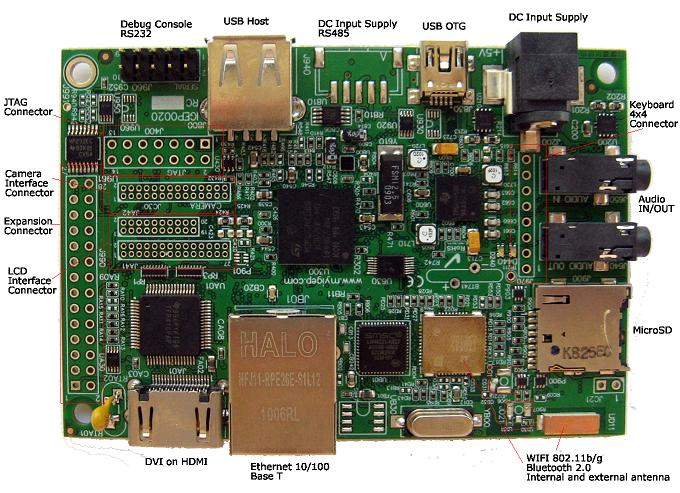
\includegraphics[width=\textwidth]{afbeeldingen/IGEPv2}
	\caption{IGEPv2 embedded computer}
\end{figure}

Dat hebben we gevonden in de vorm van de \strong{\makeurl{http://www.globalscaletechnologies.com/t-guruplugdisplaydetails.aspx}{GuruPlug Display}}. Deze computer is misschien minder krachtig (vooral acceleratiemogelijkheden zijn een prominente afwezige), maar wordt geleverd als een sluitend geheel waarbij het standaardpakket tevens voorziet van alle nodige kabels.

\begin{figure}
	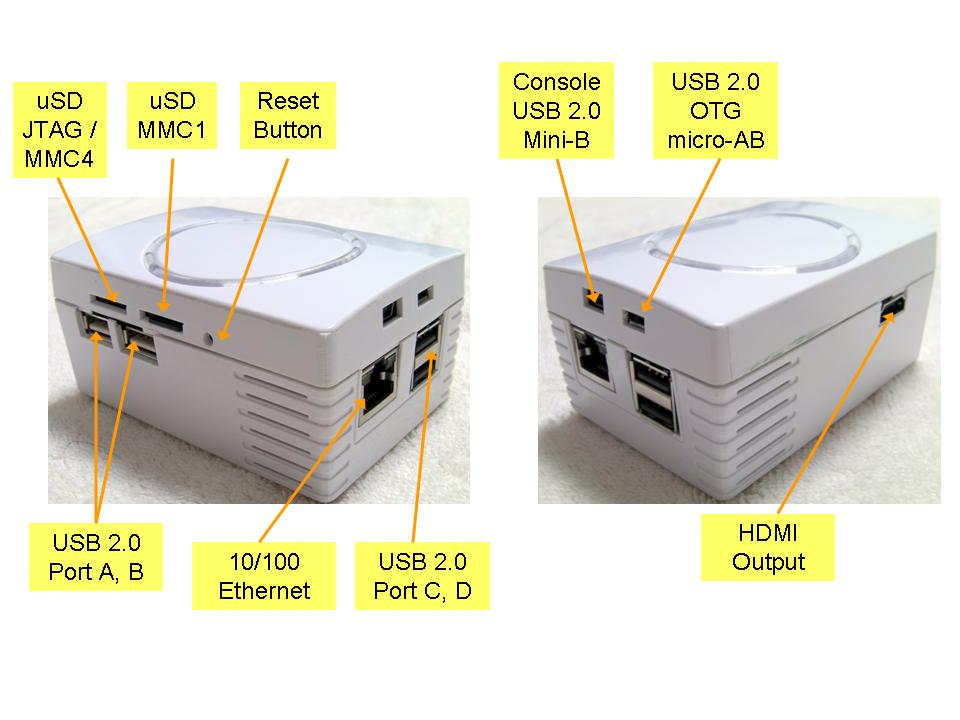
\includegraphics[width=\textwidth]{afbeeldingen/GuruPlug_Display}
	\caption{GuruPlug Display}
\end{figure}

Verschillende maanden hebben we dan ook gedacht dat we de GuruPlug Display zouden gebruiken, meer nog: we waren reeds begonnen met de ontwikkeling van een besturingssysteem voor deze hardware. Er doken echter problemen op toen we besloten de hardware aan te kopen. Vooreerst werd bij aankoop van het eerste device meer dan \euro 40 aan portkosten aangerekend, wat een significante meerkost betekende. Vervolgens liet het bedrijf achter de GuruPlugs weten dat er geen Europese modellen zouden gemaakt worden, waardoor we steeds een conversiestekker zouden moeten aankopen. Aangezien de hardware reeds niet al te performant was, hebben we wegens deze twee meerkosten besloten om opnieuw uit te gaan kijken naar een alternatieve oplossing, ondanks het feit dat we al begonnen waren met de effectieve implementatie.

Daarom zijn we op zoek gegaan naar een vergelijkbare plug-computer (zodat we niet veel werk zouden moeten herdoen), die beter leverbaar is, en dat liefst ook binnen Europa. Zo zijn we gestuit op de \strong{\makeurl{http://www.genesi-usa.com/products/efika}{EFIKA MX}} Smarttop computer, een computer vergelijkbaar met de GuruPlug. Meer zelfs, bepaalde elementen (zoals de \ac{cpu} generatie en de \ac{gpu}) hebben zelfs betere specificaties. Daartegenover staat dat er geen Bluetooth aanwezig is, alsook de prijs ietwat hoger ligt. Maar omdat Genesis een verdeler in het Verenigd Koninkrijk heeft, verdwijnt die meerkost daar we geen portkosten moeten betalen bij de uiteindelijke bestelling.

\begin{figure}
	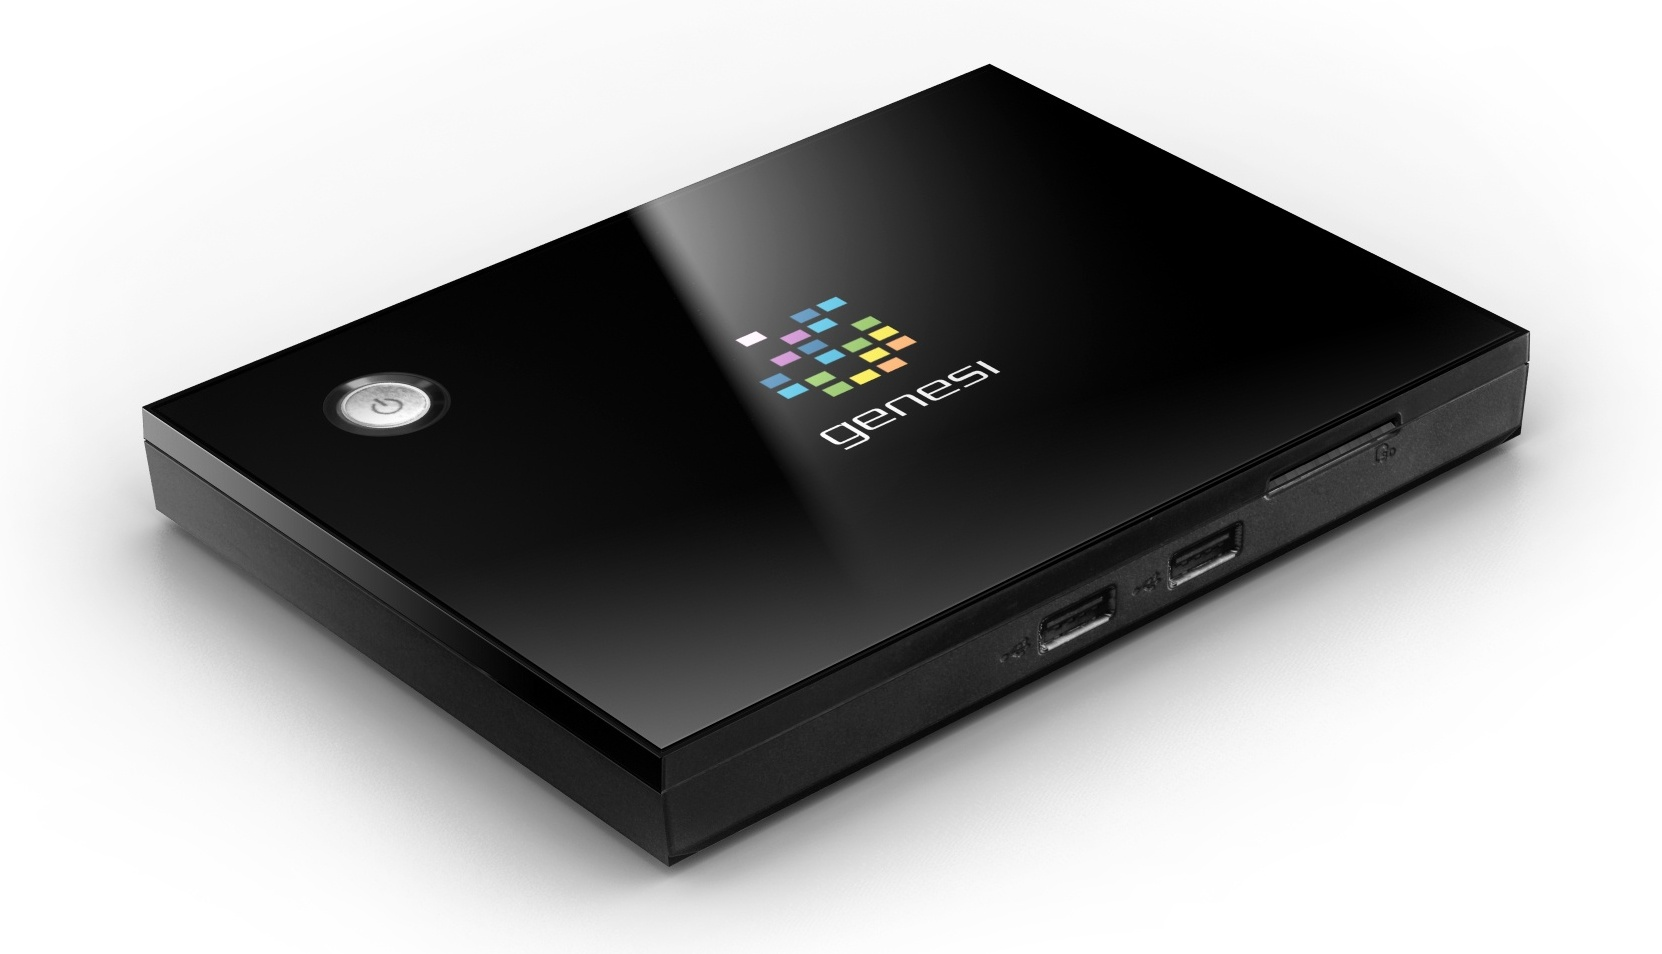
\includegraphics[width=\textwidth]{afbeeldingen/EFIKA_MX}
	\caption{Genesis EFIKA MX}
\end{figure}

\section{Inputmodule}
\label{ontwerp:hardware:input}

De gebruiksinterface wordt gerealiseerd door 4 grote drukknoppen ingebouwd in de kast van elke kiosk. Momenteel worden deze knoppen intern doorverbonden met een afstandsbediening, waardoor de gebruiker via het indrukken van de knoppen indirect de \acs{dvd}-speler kan besturen om zo een fragment te selecteren.

\begin{figure}
	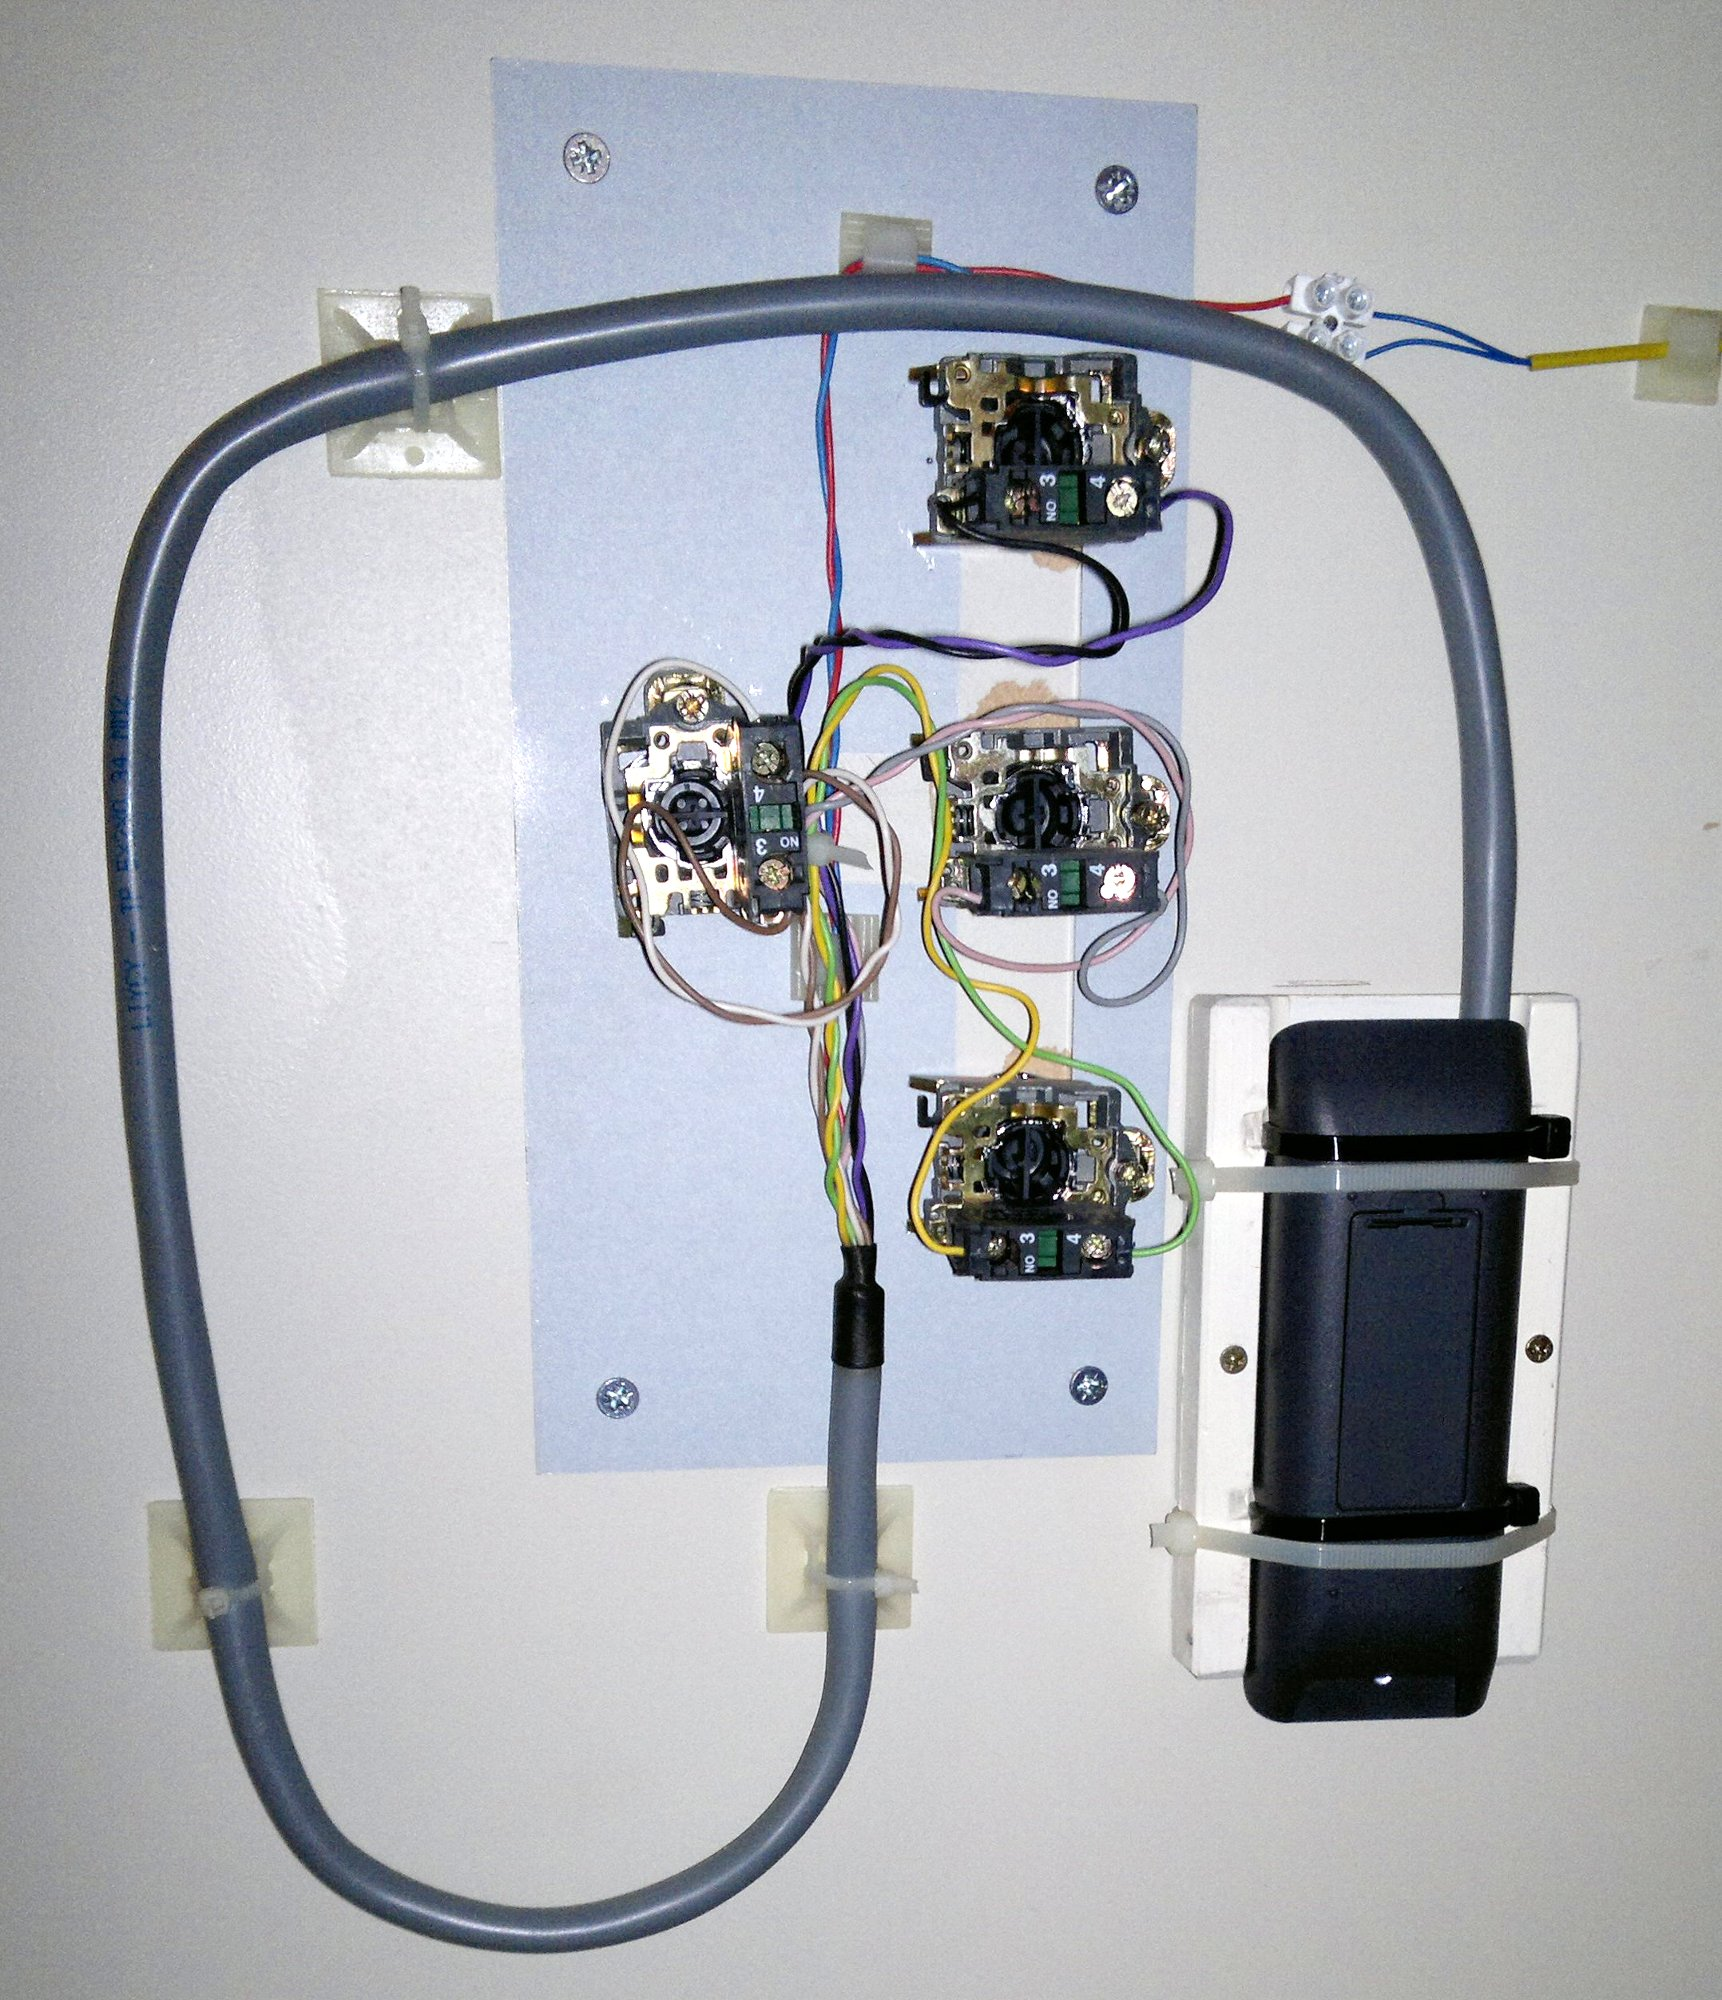
\includegraphics[width=\textwidth]{afbeeldingen/kiosk_knoppen}
	\caption{Huidige aansluitingsmethode knoppen}
\end{figure}

Nu we echter de \acs{dvd}-spelers gaan vervangen door een computer, zullen we ook voor deze inputmodule een compatibel alternatief moeten vinden. Aan deze module worden enkele specifieke eisen gesteld:
\begin{itemize}
\item Goedkoop: de module moet zo goedkoop mogelijk te produceren zijn en mag niet teveel energie verbruiken;
\item Toekomstgericht: aansluitmogelijkheden mogen geen gebruik maken van oude protocollen;
\item Gebruiksvriendelijk: installatie van de module moet eenvoudig zijn;
\item Snel: de tijd tussen het indrukken van een toets en registratie van het signaal moet minimaal zijn;
\item Uitbreidbaar: het moet mogelijk zijn om later extra toetsen aan te sluiten.
\end{itemize}

\subsection{Aansluiting}

Het grootste ontwerpprobleem hierbij is de manier van aansluiting die we zullen gebruiken om de module in verbinding te brengen met de rest van de kioskhardware. De meeste eenvoudige keuze zou die zijn van de \strong{parallelle poort}, waarbij we de pinnen van de poort vrijwel direct zouden kunnen verbinden met de knoppen. Jammer genoeg zijn parallelle poorten steeds schaarser, en komt die vrijwel nooit meer voor op embedded hardware. Een andere toegankelijke optie is de \strong{seriële poort}. Hierbij zou dan extra periferie benodigd zijn om in te staan voor de serialisatie van de signalen. Indien we echter platform-specifieke code toelaten, kunnen we de stuursignalen van de poort op een parallelle manier misbruiken zodat ook die periferie geëlimineerd wordt. Toch voldoet ook deze oplossing niet: ook de seriële poort wordt steeds schaarser, en alhoewel ze momenteel nog te vinden is op de meeste embedded-hardware bestaat de mogelijkheid dat dit binnen geringe tijd niet meer zo is.

Daarom hebben we uiteindelijk gekozen voor een poort die we normaal gezien wel nog enkele jaren zullen terugvinden op de meest courante hardware: de \ac{usb} poort. Deze veelzijdige poort laat ons toe om de inputmodule te laten communiceren met een computer, en is ook relatief toekomstgericht (de recent geïntroduceerde \ac{usb} versie 3 is nog steeds volledig terugwaarts compatibel met \ac{usb} versie 1 toestellen). Maar het gebruik van \ac{usb} kent ook een nadeel: het protocol is immers pakket-georiënteerd, waardoor extra periferie een noodzaak is. Ook is de configuratie complexer, zeker indien we een toestel willen dat zonder speciale stuurprogramma's werkt op verschillende besturingssystemen.

\subsection{Realisatie \acs{usb}-communicatie}

Aangezien \ac{usb} een pakket-georiënteerd protocol is, hebben we steeds extra periferie nodig om de gebruikersinvoer door te sturen. Om geen speciale software te vereisen moet onze module een apparaat uit de \ac{usb} \ac{hid} klasse implementeren. Voor bepaalde subcategorieën van deze klasse (zoals toetsenborden, muizen, \dots) wordt immers gegarandeerd dat compatibele besturingssystemen er mee zullen kunnen omgaan zonder daarvoor extra stuurprogramma's nodig te hebben. Daarom zullen we onze module zichzelf laten identificeren als een toetsenbord, waarbij we dan in de Javascript code van de voorstellingen gepast kunnen reageren op dergelijke toetsaanslagen. Dit vereenvoudigt ook de achterliggende applicatie, omdat we anders nog zouden moeten voorzien in code die de signalen opvangt en interpreteert, om ze dan op gepaste wijze aan te bieden aan de Javascript code van de voorstellingen.

Om een \ac{usb} toetsenbord te realiseren, zijn we in eerste instantie op zoek gegaan naar \strong{\ac{usb} keyboard encoders}. In de huidige opzet hebben we echter maar nood aan 4 knoppen, terwijl de meeste keyboard encoders veel meer toetsen toelaten. Daarom is de prijs meestal ook een pak hoger, zo kost de \makeurl{http://www.ultimarc.com/ipacve.html}{I-Pac VE} keyboard encoder, die 32 toetsen toelaat, reeds \$35!

Daarom lijkt het interessanter om zelf te voorzien in de conversie naar \ac{usb}-pakketten, door gebruik te maken van een \strong{microcontroller met \ac{usb} hardware}. Dergelijke microcontrollers voorzien in on-chip \ac{usb} communicatiemogelijkheden, net zoals de meeste reguliere microcontrollers toelaten om gegevens over een seriële \ac{uart} te transporteren. Om vervolgens de \ac{usb} hardware op een toegankelijke manier te gebruiken, bestaan er verschillende bibliotheken zoals de officiële \ac{usb} bibliotheek van Atmel, of het open-source \makeurl{http://www.fourwalledcubicle.com/LUFA.php}{\ac{lufa}}. Het nadeel van deze piste is echter de meerkost van de \ac{usb} hardware, die eigenlijk onnodig is daar we enkel gebruik zullen maken van de \emph{low speed} overdrachtsmodus.

Een derde optie is om gebruik te maken van een \strong{microcontroller met \ac{usb} software}. Hierbij hebben we geen speciale hardware nodig, enkel een microcontroller die krachtig genoeg is om de \ac{usb} software uit te voeren. Het grote nadeel hieraan is dat het met de huidige microcontrollers enkel mogelijk is om gebruik te maken van \emph{low speed} \ac{usb}, maar voor onze toepassing is dit geen probleem. Opnieuw zijn er verschillende mogelijkheden om dit te realiseren, waarvan er een beschreven is in een \makeurl{http://www.atmel.com/dyn/resources/prod\_documents/doc2556.pdf}{\emph{application note}} van Atmel. Deze application note gebruikt relatief weinig hardware om elementaire \ac{usb} communicatie te realiseren, maar zoals later zal blijken zijn er zelfs nog efficiëntere configuraties mogelijk. Ook is de software geschreven in AVR assembler, waardoor het geheel niet zo overdraagbaar is. Daarom zullen we gebruik maken van een open-source alternatief: de \makeurl{http://www.obdev.at/products/vusb/index.html}{V-USB} bibliotheek. Deze in C-geschreven bibliotheek biedt een eenvoudigere interface en daarbij ook verschillende voorbeeldprojecten om het gebruik ervan te illustreren.


%
% Licenties
%

\chapter{Licenties}
\label{ontwerp:licenties}

De keuze van een goede licentie is een element waar we niet te snel mogen over gaan. Elke licentie heeft immers verschillende vereisten en gevolgen, en ook onze eigen eisen verschillen van component tot component. Terzelfdertijd moet de gekozen licentie compatibel zijn met de verschillende bibliotheken die we gebruiken binnen de verschillende componenten. Ook willen we het eindresultaat openstellen voor open-source gebruik, waar zouden we anders staan moesten anderen dit nooit gedaan hebben. Tenslotte willen we ook de piste naar eventuele commercialisering open houden.

Het lijkt misschien moeilijk, al dan niet onmogelijk om hier allemaal rekening mee te houden, vooral als we tegelijk spreken over eventuele commercialisering en het product open-source maken. Toch is dit perfect mogelijk, en zijn er genoeg succesverhalen om dat mee te illustreren.

\section{Types licenties}
\label{ontwerp:licenties:type}

Vooraleer dieper in te gaan op hoe we open-source licenties kunnen gebruiken, is het interessant om een grove indeling te maken en zo enkele terugkerende eigenschappen te beschrijven. Hierbij identificeren we drie soorten open-source software: die in het publieke domein, die onder een permissive licentie, en die onder een copyleft licentie \citep{fsf:categories}.

\subsection{Copyleft licenties}
\label{ontwerp:licenties:type:copyleft}

Bij dergelijke licenties wordt het copyright van de auteur gebruikt om te zorgen dat het herdistribueren van het product of een gewijzigde versie daarvan enkel gebeurt onder dezelfde of een compatibele licentie. Hiermee kan een auteur bijvoorbeeld erop toezien dat software die hij vrijgeeft, ook altijd vrij zal blijven. Bekende voorbeelden van deze licentie zijn de \ac{gpl}, of de \ac{cc-sa} licentie.

Binnen deze categorie maken we ook nog een onderscheid of het gaat over ``weak'' of ``strong'' copyleft. Het verschil ertussen vindt men op vlak van afgeleid werk. Meer bepaald, in het geval van weak copyleft vereist men niet dat het volledige product onder copyleft valt indien men enkel gebruik maakt van een project dat onder een copyleft licentie valt. Als dat project echter onder een strong copyleft licentie zou vallen, moet het volledige eindresultaat vrijgegeven worden onder een compatibele copyleft licentie.
Dit onderscheid is vooral van belang bij libraries: als die onder een weak copyleft licentie valt kan men de library gebruiken zonder de volledige applicatie te moeten vrijgeven. Wijzigingen aan de code zélf moeten echter wel vrijgegeven worden. Voorbeelden van weak copyleft licenties zijn de \ac{lgpl} en de \ac{mpl}.

Net zoals de \ac{lgpl} specificeert dat afgeleid werk niet onder de copyleft clausule valt, laat men bij de afgeleide \ac{agpl} deze eis vallen voor gebruik over het netwerk. Dit is vooral interessant voor webservices; moesten deze immers onder de \ac{gpl} vallen dan zou ook elke applicatie die ervan gebruik maakt onder een \ac{gpl} compatibele licentie moeten vrijgegeven worden.

\subsection{Permissive licenties}
\label{ontwerp:licenties:type:permissive}

Hierbij is het niet langer vereist om wijzigingen aan de code vrij te geven. Daardoor kan het dus zijn dat projecten die onder deze licentie vallen, gebruikt worden binnen proprietaire producten en dit zelfs zonder eventuele wijzigingen aan die code te moeten vrijgeven. Vaak komen de licenties echter wel met een extra vereiste, maar die houdt vaak niet veel in. Zo stelt de \ac{mit} licentie dat de tekst ervan moet meegeleverd worden met het eindproduct, de Apache licentie eist datzelfde van een copyright notice en de disclaimer.

\subsection{Licenties zonder copyright}
\label{ontwerp:licenties:type:public}

Hoewel permissive licenties weinig of geen restricties stelden aan het gebruik van de code, blijft het copyright steeds in handen van de originele auteur. Indien we ook dit afstaan kan en mag iedereen om het even wat doen met de code. Volledig het copyright afstaan, waarbij de code in het \emph{public domain} terechtkomt, is echter een complexe zaak: de situatie moet bekeken worden van land tot land, en soms is het zelf onmogelijk om de auteursrechten volledig af te staan.

Er bestaan verschillende licenties die code toekennen aan het public domain, waaronder de CreativeCommons Zero licentie en de \ac{wtfpl}.

\section{Open-source software commercialiseren}
\label{ontwerp:licenties:commercialiseren}

Vaak wordt er met schrik gekeken naar open-source licenties omdat ze maar moeilijk passen binnen conventionele businessmodellen. Toch is het perfect mogelijk om dergelijke software te commercialiseren, mits een geschikte aanpak. We gaan nu twee dergelijke schema's beschrijven, met telkens een bedrijf dat dit ook succesvol toegepast heeft als illustratie.

\subsection{Ondersteuning leveren}
\label{ontwerp:licenties:commercialiseren:ondersteuning}

Een model dat vaak toegepast wordt door fabrikanten van Linuxdistributies is het leveren van ondersteuning naast een gratis product. Een mooi voorbeeld hiervan is Red Hat, die verantwoordelijk is voor de \ac{rhel} distributie. Aangezien \ac{rhel} gebaseerd is op Linux en andere open-source componenten waarvan de overgrote meerderheid valt onder een copyleft of permissive licentie, mag Red Hat niet zomaar zijn product verkopen zonder er de broncode van vrij te geven. Toch zijn er veel diensten die Red Hat wel mag verkopen zonder enige bijkomende verplichting:
\begin{itemize}
  \item Toegang tot servers die updates verschaffen;
  \item Hulp bij installatie;
  \item Zelfgeschreven documentatie;
  \item Hardware (installatieschijven, \ldots).
\end{itemize}

Het is duidelijk dat \ac{rhel} een duidelijke meerwaarde heeft, ondanks het feit dat de broncode publiek beschikbaar is. Meer nog, het openen van de code naar een breder publiek opent verschillende opportuniteiten: externe programmeurs kunnen code toedragen, problemen worden sneller gevonden door het grotere testpubliek, \ldots

Een interessante opmerking is dat Red Hat wel het handelsmerk bezit op de naam \acl{rhel}. Het is dus perfect mogelijk om de broncode van \ac{rhel} te downloaden en een eigen product te lanceren, maar dit mag dan niet geadverteerd worden als zijnde \ac{rhel}. Dergelijke ``klonen'' bestaan ook, twee bekende voorbeelden zijn CentOS en \ac{sl}. Hoewel deze distributies gebaseerd zijn op dezelfde basissoftware, zijn het door de herimplementatie van de verschillende diensten die Red Hat commerciëel levert, toch heel andere producten.

\subsection{Herlicentiëren onder betaling}
\label{ontwerp:licenties:commercialiseren:herlicentieren}

Een tweede model berust op het feit dat commerciële partijen vaak geïnteresseerd zijn in non-copylefted software. We illustreren dit opnieuw met een concreet voorbeeld: het Qt framework dat ontwikkeld wordt door Nokia en uitgegeven wordt door Digia. Qt is beschikbaar onder verschillende licenties: een weak copyleft licentie, en een proprietaire licentie\footnote{Hoewel de site van Qt een ``commerciële licentie'' vermelt, gebruiken we de term ``proprietaire licentie'' omdat copylefted code ook perfect gecommercialiseerd kan worden (zie \ref{ontwerp:licenties:commercialiseren:ondersteuning}).}. Dankzij de weak copyleft licentie kan iedereen Qt downloaden, en er open-source of commerciële applicaties met maken. Dankzij de weak copyleft licentie moeten eventuele wijzigingen aan de Qt code wel steeds vrijgegeven worden.

Bedrijven hebben dit laatste vaak niet graag, ze willen wijzigingen kunnen doorvoeren aan de interne Qt code zonder die vervolgens te moeten publiceren. En dat is net waar Digia geld uit slaat: een bedrijf kan Qt gebruiken onder een proprietaire licentie, als het daarvoor betaalt.

Hoe men net die conversie naar een commerciële licentie bekomt, kan op verschillende manieren. Als de auteur van de software in kwestie nog het volledige copyright bezit is het voor hem geen probleem om de licentie te veranderen. Van zodra er verschillende auteurs zijn wordt het echter complexer. Binnen een bedrijf is het logisch dat de code die een werknemer schrijft eigenlijk eigendom is van het bedrijf. Maar van zodra er externe auteurs zijn, wat vaak het gevolg is bij een open-source project, moeten er andere maatregelen getroffen worden om de code onder meerdere licenties te kunnen vrijgeven. De piste die Nokia en Digia gekozen hebben is die van een ``contribution agreement''. Hierbij staat een auteur toe dat zijn code kan gelicencieerd worden onder een proprietaire licentie. Andere bedrijven kiezen voor een rigide ``copyright assignment'', waarbij het copyright van de code volledig doorgegeven wordt aan het bedrijf in kwestie. Het ``voordeel'' van dit laatste is dat het bedrijf geen enkele verplichting heeft en later de licentie perfect kan veranderen. Bij een contribution agreement kan dit beperkt worden: in het geval van Qt wordt bijvoorbeeld gesteld dat de code en alle wijzigingen eraan steeds beschikbaar zullen blijven onder een copyleft licentie.

Merk op dat dit model enkel mogelijk is wanneer de code geen gebruik maakt van strong copylefted code. Als dit wel het geval is, kan de software nooit onder een proprietaire licentie verspreid worden.

\section{Keuze van licenties}
\label{ontwerp:licenties:keuze}

\subsection{Software}
\label{ontwerp:licenties:keuze:software}

Voor de applicaties die we ontwerpen voor dit project hebben we steeds gekozen voor een gepaste copyleft licentie. Door de code zomaar gratis op het internet te zetten krijgt het project extra visibiliteit en is het voor een derde partij gemakkelijker om het project op te pikken en te kijken of het wel past binnen zijn omgeving. Als die partij ook uiteindelijk besluit om met onze applicaties aan de slag te gaan, kan het daarbij verschillende pistes volgen:
\begin{enumerate}
  \item Het bedrijf gebruikt en adapteert onze code om binnen zijn omgeving te werken, en wordt daarbij door de licentie verplicht de wijzigingen terug te geven aan het project;
  \item Het bedrijf zou onze code willen gebruiken, maar heeft daarvoor extra ondersteuning nodig;
  \item Het bedrijf wil de code onder een proprietaire licentie verkrijgen om zo naar believen wijzigingen te kunnen doorvoeren.
\end{enumerate}
Elk van deze mogelijkheden komt het project ten goede: of er wordt code teruggegeven, of er wordt betaald voor bepaalde diensten. Wanneer het moment komt dat een externe partij code wil toedragen aan het project zullen we wel moeten zorgen voor een gepaste contribution agreement of zelfs copyright assignment, zodat het voor ons mogelijk blijft de code uit te geven onder een gesloten licentie voor proprietair gebruik.

\subsubsection{Serverapplicatie}
\label{ontwerp:licenties:keuze:software:server}

Voor deze applicatie lijkt een strong copyleft licentie de beste keuze. Een uitzonderingsmodule voor netwerkgebruik is hier niet echt nuttig aangezien de serverapplicatie eigenlijk methodes aanroept op de kioskapplicatie en zelf geen interface aanbiedt. Wanneer we later gebruik maken van een serverside \ac{svn} library om de repository te integreren binnen de serverapplicatie, zullen we wel nood hebben aan deze uitzonderingsmodule.

Laten we eerst kijken naar de externe projecten die we gebruiken binnen de applicatie:
\addtocounter{footnote}{1}
\footnotetext[\value{footnote}]{Dit is een permissive licentie die vereist dat naast een copyright notice en de disclaimer ook de documentatie steeds ter beschikking is.}
\addtocounter{footnote}{1}
\footnotetext[\value{footnote}]{Dit is een strong copyleft licentie waarbij bundeling onder een proprietaire licentie mogelijk is mits expliciete toestemming van TMate.}
\addtocounter{footnote}{-1}
\begin{table}[h!]
  \begin{center}
    \begin{tabular}{c c}
    Project & Licentie \\
    \hline
    log4j & Apache License versie 2.0 \\
    Tomcat & Apache License versie 2.0 \\
    Apache Commons & Apache License versie 2.0 \\
    Subversion & Apache License versie 2.0 \\
    XPP & Indiana University Extreme! Lab Software License$^{\decimal{footnote}}$\addtocounter{footnote}{1} \\
    JWt & \ac{gpl} versie 2 \\
    \end{tabular}
  \end{center}
  \caption{Open-source projecten binnen de serverapplicatie}
\end{table}

\paragraph{Licentie} Om een licentie te kiezen moeten we nauwgezet analyseren met welke projecten die licentie compatibel is.  We willen bijvoorbeeld nagaan of we ons project kunnen distribueren onder de \ac{gpl}. De Apache 2 licentie is enkel compatibel met versie 3.0 van de \ac{gpl} \citep{fsf:comments}, en de \makeurl{http://www.extreme.indiana.edu/viewcvs/~checkout~/XPP3/java/LICENSE.txt}{Indiana University Extreme! Lab Software License} is een permissive licentie waardoor ze vast en zeker compatibel is met de \ac{gpl}. Het is dus duidelijk dat we de serverapplicatie enkel onder versie 3 van de \ac{gpl} (of afgeleiden) kunnen uitgeven.

\paragraph{Herlicentiëren} Zoals beschreven in sectie \ref{ontwerp:licenties:commercialiseren:herlicentieren} willen we het mogelijk houden om onder betaling de code onder een proprietaire licentie te verkopen. Niet alle projecten die we hergebruiken zijn echter compatibel met een dergelijke licentie! Voor de projecten onder een permissive licentie (log4j, Tomcat, Apache Commons, XPP) is er geen probleem, we moeten enkel zorgen dat we voorzien in de tekst van de licentie, een copyright notice, en eventueel andere documenten. Maar het laatste project, JWt, valt onder de strong copyleft \ac{gpl} die niet compatibel is met een proprietaire licentie. Als we beter kijken zien we echter dat ze hetzelfde model hanteren als dat wij beschreven hebben in sectie \ref{ontwerp:licenties:commercialiseren:herlicentieren}: mits betaling is het mogelijk om dezelfde code te verkrijgen onder een proprietaire licentie. Als we dus de code van JWt aankopen is het perfect mogelijk om onze serverapplicatie te verkopen onder een proprietaire licentie.

\subsubsection{Kioskapplicatie}
\label{ontwerp:licenties:keuze:software:kiosk}

Opnieuw zullen we kijken in welke mate we een strong copyleft licentie kunnen toepassen op onze code. Aangezien de kioskapplicatie een \ac{upnp} service aanbiedt, zullen we nu echter wel aandacht moeten besteden aan de \ac{agpl}, die een copyleft uitzonderingsclausule voor netwerkgebruik aan boord heeft.

Vooreerst kijken we naar de licenties van externe projecten die we gebruiken:
\begin{table}[h!]
  \begin{center}
    \begin{tabular}{c c}
    Project & Licentie \\
    \hline
    Log4Qt & Apache License versie 2.0 \\
    BRisa UPnP & \ac{lgpl} 3.0 \\
    Qt & \ac{lgpl} versie 2.1 en 3.0 \\
    libqxt & \ac{lgpl} versie 2.1 \\
    \end{tabular}
  \end{center}
  \caption{Open-source projecten binnen de kioskapplicatie}
\end{table}

\paragraph{Licentie} De situatie is hier iets eenvoudiger dan bij de serverapplicatie. Door het gebruik van een project dat valt onder versie 2.0 van de Apache License, kunnen we eigenlijk al maar enkel gebruik maken van versie 3.0 van de \ac{gpl}. Die licentie is vervolgens compatibel met de overige licenties waarvan we gebruik maken.

Maar aangezien de applicatie een webservice aanbiedt wilden we gebruik maken van de \ac{agpl}. Als we in detail kijken naar de tekst van die licentie zien we dat vanaf versie 3 er in beide licenties een expliciete clausule \citetext{\citealp[sectie 13]{fsf:gpl}; \citealp[sectie 13]{fsf:agpl}} is opgenomen die ze compatibel maakt. Daardoor kunnen we zonder probleem de code onder versie 3 van de \ac{agpl} laten vallen.

\paragraph{Herlicentiëren} Ook dit aspect is gemakkelijker voor de kioskapplicatie. Een proprietaire licentie is immers toegelaten door de permissive licentie waaronder Log4Qt valt, en de overige projecten gebruiken een weak copyleft licentie die expliciet stelt dat copyleft niet van toepassing is indien we enkel linken met de code. Wijzigingen aan de code zelf moeten wel vrijgegeven worden, maar dat hebben we ook gedaan (zie deel \ref{kiosk}).

\subsubsection{Firmware inputmodule}
\label{ontwerp:licenties:keuze:software:inputmodule}

De firmware maakt maar gebruik van 1 extern project: V-USB. Dit project valt opnieuw onder een duale licentie: enerzijds de \ac{gpl}, en anderzijds een licentie die mits betaling gebruik binnen een proprietair project toelaat.

\paragraph{Licentie} De situatie is hier vrij eenvoudig: we moeten enkel compatibel zijn met de \ac{gpl} waaronder het V-USB project valt. Daarom zullen we zelf ook kiezen om gebruik te maken van de \ac{gpl}.

\paragraph{Herlicentiëren} Net zoals bij JWt valt V-USB onder een duale licentie waardoor gebruik binnen een proprietair project enkel mogelijk is mits aankoop van de code onder een compatibele licentie.

\subsection{Hardware inputmodule}
\label{ontwerp:licenties:keuze:hardware}

Aangezien veel van de termen die gebruik worden binnen software-georienteerde licenties zoals de \ac{gpl} niet van toepassing zijn op hardware (zo is het bij software al moeilijk genoeg om ``afgeleid werk'' nauwkeurig te omschrijven), kiezen we ervoor om gebruik te maken van een licentie die specifiek ontworpen is voor open-source hardware. Toch willen we niet teveel afwijken van het strong copyleft principe, aangezien dat een elementair deel is van het business model achter dit project. Daarom maken we gebruik van \makeurl{http://www.ohwr.org/attachments/662/CERNOHLv1\_1.pdf}{versie 1.1 van de CERN \ac{ohl}}, een strong copyleft licentie specifiek ontworpen voor hardware. We halen snel de belangrijkste elementen van de licentie aan:

\begin{itemize}
  \item Copyright en handelsmerken blijven behouden bij de originele auteur;
  \item Distributie van het project is toegelaten, maar in het geval van wijzigingen moeten de designdocumenten toegankelijk zijn en onder een compatibele licentie vrijgegeven worden;
  \item Productie en distributie van de hardware is toegelaten.
\end{itemize}

Hoewel commercialisering van dit product hiermee mogelijk is, zoals altijd kunnen we de licentie veranderen naar iets dat compatibel is met proprietair gebruik, is de kans klein dat we dit ooit zullen moeten doen. Het product is immers zo specifiek aan de situatie waarbinnen het gebruikt wordt dat het wellicht weinig nut zal hebben buiten de MIRA.

\subsection{Scriptie}
\label{ontwerp:licenties:keuze:scriptie}

Het laatste item waar we een gepaste licentie moeten voor vinden, is dit document zelf. Hierbij hebben we een ander doel voor ogen dan bij de software en hardware: eventuele commercialisering is niet relevant. Het zou ook interessant zijn om gequote te kunnen worden zonder dat daarbij het werk waarin de quote terecht komt onder dezelfde termen moet vrijgegeven worden. Een copyleft licentie is dus niet gewenst, maar ook de meeste permissive licenties zijn te software georienteerd om op een zinnige manier toegepast te kunnen worden op dit document.

Een verzameling licenties die vaak gebruikt worden buiten de softwarewereld, zijn de \makeurl{https://creativecommons.org/}{\acl{cc}} licenties. Deze licenties bevatten weinig of geen termen die specifiek zijn aan software, en werken volgens een modulair principe: afhankelijk van de specifieke eisen van de auteur kiest hij voor een aantal plugins die het hergebruik van zijn werk beperken. Zo zijn er de volgende plugins:
\begin{itemize}
  \item Attribution (BY): de auteur moet altijd expliciet vermeld blijven;
  \item Noncommercial (NC): het werk mag niet gebruikt worden voor commerciële doeleinden;
  \item No derivative works (ND): enkel exacte kopieën van het werk mogen gedistribueerd worden;
  \item Share-alike (SA): het werk moet onder een vergelijkbare licentie verdeeld worden (cfr. copyleft).
\end{itemize}

Voor deze scriptie willen we enkel dat de auteur correct geattribueerd wordt indien er naar het werk verwezen wordt of er fragmenten uit gebruikt worden. Daarom zullen we kiezen voor de \ac{cc-by} licentie. We hebben gekozen voor een oudere versie van deze licentie, namelijk versie 2.0 in plaats van versie 3.0, omdat er enkel van die versie een Belgische versie bestaat.

\part{Server}
\label{server}

\chapter{Structuur}
\label{server:structuur}

Op het hoogste niveau hebben we de serverapplicatie onderverdeeld in enkele logische subsystemen, zijnde het netwerk en de repository. Onderling communiceren deze subsystemen niet met elkaar: coördinatie verloopt door een overkoepelende controller. Zo is het mogelijk om elk subsysteem als een alleenstaand geheel te behandelen, wat het ontwikkelingsproces sterk vereenvoudigt. Tenslotte is er nog de webinterface, die dezelfde visibiliteit heeft als de controller: acties die een gebruiker uitvoert op de beheerinterface kunnen een impact hebben op objecten binnen het netwerk of de repository.

Om code te abstraheren en controle van subsystemen te vereenvoudigen moet elk van de subsystemen een bepaalde klasse uitbreiden met de concrete implementatie. Die klasse voorziet niet alleen in bepaalde gedeelde functionaliteit (zoals het genereren van log berichten, of inladen van de nodige configuratiebestanden), maar schrijft ook voor hoe de effectieve implementatie moet gevormd worden. Hierdoor wordt het eenvoudig om vanuit de applicatiecontroller op een eenduidige manier bepaalde standaardacties (zoals het opstarten of afsluiten van een subsysteem) uit te voeren.

\section{Netwerk subsysteem}
\label{server:structuur:netwerk}

Het netwerk subsysteem verzorgt wat we in de vorige hoofdstukken tot applicatieprotocol gedoopt hebben. Het subsysteem is opgesplitst in enkele samenwerkende componenten: vooreerst is er het gedeelte dat dient als main entrypoint voor andere componenten die willen gebruik maken van het netwerksubsysteem. Daartoe biedt het bijvoorbeeld een lijst van aanwezige kiosken, en kan voor elke kiosk een object opgevraagd worden dat toelaat om gegevens op te halen of acties uit te voeren. Ook is er voorzien in de nodige functionaliteit om signalen door te geven, bijvoorbeeld om geschikt te reageren op de toevoeging van een nieuwe kiosk.
Door al deze functionaliteit te bundelen in een enkele klasse, is dit de enige interface tussen het volledige subsysteem en de rest van de applicaties. De uiteindelijke implementatie van het subsysteem kan hierdoor eenvoudig gewijzigd worden, zonder veel te moeten veranderen aan componenten die gebruik maken van dit systeem.

Het netwerk subsysteem bevat ook nog een gedeelte dat instaat voor de effectieve monitoring van het netwerk, door te reageren op signalen van de achterliggende \ac{upnp} bibliotheek. Dit gedeelte is puur intern, en het is niet de bedoeling dat een externe component communiceert met deze netwerk monitor. Als de monitor bepaalde informatie wil vrijgeven aan de buitenwereld (wat bijvoorbeeld voorkomt als het een nieuwe kiosk detecteert), zal het dit doorgeven aan de publieke component van het netwerk subsysteem, waarna die bijvoorbeeld bepaalde signalen zal uitsturen. Hoewel dit geconvolueerd mag lijken is dit een heel interessant design: zoals hierboven vermeld mogen we nu steeds de monitor naar believen aanpassen; zolang de publieke interface maar dezelfde blijft zal niemand hier iets merken.

Om het voor de buitenwereld eenvoudig te maken om te interfacen met het netwerk, zal de publieke interface niet alleen informatie vrijgeven maar ook toegang bieden tot functionele objecten die eenvoudige manipulatie van hun onderwerp toelaten. Zo zal een \code{Network::getDevice(String uuid)} aanroep niet louter informatie over het toestel teruggeven, maar een volwaardig \code{Device} object. Dit object kan dan gebruikt worden om het toestel zelf te manipuleren: indien we bijvoorbeeld over een kiosk spreken zal het voorzien zijn van een \code{Device::Shutdown} methode.

\section{Repository subsysteem}
\label{server:structuur:repository}

Dit systeem dient als wrapper rond de repository waarbinnen alle gegevens van het systeem (configuraties en voorstellingen) opgeslagen zijn. Zoals vermeld in hoofdstuk \ref{ontwerp} staat de server in voor het ophalen en verwerken van de configuratiegegevens, en moet het de nodige kiosken laten weten wanneer de media die ze tonen gewijzigd zijn.

Net zoals bij het netwerk subsysteem biedt het repository subsysteem een publieke interface die de buitenwereld toelaat gegevens op te vragen. Ook zullen de teruggegeven objecten opnieuw gesofisticeerd zijn om eenvoudig verwerken van de gegevens toe te laten: de \code{Repository::getConfiguration(String id)} aanroep bijvoorbeeld zal daarom een \code{KioskConfiguration} object teruggeven hetwelk specifieke functies bevat zoals \code{getVolume}. Hoewel dit systeem zijn nadelen kent -- een wijziging van het configuratieformaat vereist direct wijzigingen aan de servercode -- zorgt de rigide opzet ervoor dat inconsistenties tussen de repository en de achterliggende logica snel zullen duidelijk worden. 

Bij het opstarten van het repository subsysteem zal een initiële \code{checkout} uitgevoerd worden. Hierna zal een interne timer gestart worden die om de minuut controleert of er geen nieuwe revisie in de repository te vinden is. Indien dat het geval is, zullen alle configuraties opnieuw binnengehaald worden om dan eventueel de wijzigingen naar een client te sturen. Momenteel gebeurt dit echter vrij inefficiënt: alle configuraties worden opnieuw opgehaald en verstuurd, los van het feit of er ook effectief wijzigingen gebeurd zijn. Voor een volgende versie streven we ernaar om ook effectief de delta-gegevens te interpreteren en zo intelligent de nodige veranderingen door te sturen.

\section{Applicatiecontroller}
\label{server:structuur:controller}

Dit systeem staat in voor de coördinatie van acties die niet geïsoleerd blijven tot een enkel subsysteem. Het beste voorbeeld hiervoor is wanneer het netwerk subsysteem een nieuwe component detecteert. Om de code overzichtelijk te houden zal het netwerk subsysteem dan geen actie ondernemen, maar louter zijn gegevens updaten en een signaal uitsturen. De applicatiecontroller vangt tenslotte dit signaal op om vervolgens de repository te raadplegen voor eventuele configuratiegegevens.

\section{Website subsysteem}
\label{server:structuur:website}

Deze component visualiseert de gegevens uit de repository en netwerk subsystemen, en laat de gebruiker toe om er controle over uit te oefenen. Die controle is echter beperkt: persistente configuratie moet nog altijd verlopen via manuele interventie.

\chapter{Realisatie}
\label{server:realisatie}

\section{Statische codeanalyse}
\label{server:realisatie:codeanalyse}

Om de kwaliteit van de code systematisch op te drijven, hebben we gebruik gemaakt van statische codeanalyse. Daarbij analyseert een applicatie de code zonder die ook effectief uit te voeren, om vervolgens een verslag te kunnen opbouwen waarbij de inhoud verschilt van applicatie tot applicatie.

\subsection{Stijl}
\label{server:realisatie:codeanalyse:stijl}

Een eerste soort van statische codeanalyse-applicaties toetst de codebase aan een verzameling regels om zo een uniforme codestijl te bekomen. Dit lijkt misschien niet zo nuttig, maar leesbare code en een uniforme codestijl maakt het veel eenvoudiger om de applicatie te onderhouden.
Voor Java bestaat er zo een heel krachtige applicatie, \makeurl{http://checkstyle.sourceforge.net/}{Checkstyle}, die geleverd wordt met een enorm uitgebreide set aan modules die elk een bepaald aspect analyseren. Om nog verfijnder tewerk te gaan kunnen we elke module vaak beperken met een aantal filters, zodat we bijvoorbeeld eenvoudig kunnen stellen dat de publieke methodes van een interface voorzien moeten zijn van Javadoc.

De standaardconfiguratie van Checkstyle is vrij strikt, waardoor een eerste controle van de serverapplicatie meer dan 1500 waarschuwingen opleverde. Daarom hebben we een eigen configuratie aangemaakt, gebaseerd op de standaardconfiguratie met de strengste eisen (zoals het beperken van de lijnlengte, of het verbieden van elk teveel aan spaties) wat versoepeld. Ook hebben we enkele eigen regels toegevoegd om praktijken die we reeds uitvoerden nu ook systematisch te kunnen controleren. Zo hebben we bijvoorbeeld een regel toegevoegd die bepaalt dat variabelen binnen een klasse geprefixt moeten worden met een kleine ``m'', parameters van een functie een ``i'' voor hun naam moeten krijgen, en lokale variabelen altijd met een ``t'' moeten beginnen. De configuratie van die ene regel is te zien in fragment \ref{lst:checkstyle:variabelen}.

\begin{lstlisting}[language=XML, float, caption=Checkstyle configuratie voor de naamgeving van variabelen., label=lst:checkstyle:variabelen]
<module name="LocalVariableName">
  <property name="format" value="^t[A-Z][a-zA-Z0-9]*$"/>
</module>
<module name="ParameterName">
  <property name="format" value="^i[A-Z][a-zA-Z0-9]*$"/>
</module>
<module name="MemberName">
  <property name="format" value="^m[A-Z][a-zA-Z0-9]*$"/>
</module>
\end{lstlisting}

\subsection{Correctheid}
\label{server:realisatie:codeanalyse:correctheid}

Dergelijke applicaties gaan op zoek naar logische fouten in de code, waarbij de code wel legaal is maar ze bijvoorbeeld de applicatie doet crashen wanneer ze uitgevoerd wordt. Het is duidelijk dat dit een zeer complexe definitie is, die veel gesoftisticeerdere regels en heuristieken vereist dan wanneer men louter de codestijl wil controleren. Het probleem met zulke applicaties is dan ook dat er vaak een lage \emph{signal to noise} verhouding is: of er worden veel valse positieven gedetecteerd, of veel fouten worden helemaal niet gevonden.

Om toch zoveel mogelijk fouten te vinden via statische analyse, hebben we gebruik gemaakt van meerdere tools. Vooreerst hebben we gekeken naar \makeurl{http://findbugs.sourceforge.net/}{FindBugs}, een tool die zoals de naam laat uitschijnen vooral op zoek gaat naar echte fouten. Hoewel de \makeurl{http://findbugs.sourceforge.net/bugDescriptions.html}{databank aan regels} die het daarbij gebruikt vrij uitgebreid is, had FindBugs niet veel te zeggen over onze code. We hopen dat dit een teken is dat de codebase van goede kwaliteit is.

Een andere applicatie die we gebruikt hebben is \makeurl{http://pmd.sourceforge.net/}{PMD}. Deze gaat niet alleen op zoek naar bugs, maar ook naar verkeerd gebruik van geheugen, overdreven complexe codefragmenten, suboptimale code, en code die nooit uitgevoerd wordt (\emph{dead code}). Zo hebben we met behulp van PMD verschillende suboptimale \emph{inner loops} kunnen versnellen, alsook enkele complexe klassen vereenvoudigd. Kritieke fouten zijn er echter opnieuw niet gevonden.

\chapter{Deployment}
\label{server:deployment}

\section{Besturingssysteem}
\label{server:deployment:besturingssysteem}

Zoals wel vaker het geval is, is de keuze van het besturingssysteem beperkt geweest door de hardware waarop het moest draaien. Zo komt de Synology DS207+ wel met een Linux-distributie, maar is die zodanig geconfigureerd dat we eigenlijk liever zouden uitwijken naar een meer \emph{general purpose} embedded distributie. Hierbij denken we bijvoorbeeld aan de vele foto-, muziek- en videoapplicaties die standaard op het toestel staan, of aan de zeer mooie maar even nutteloze webinterface die het toestel aanbiedt.

Maar zomaar even een andere distributie installeren is helemaal niet zo eenvoudig. Omdat het hier om een zeer specifiek toestel met beperkte hardware gaat, kunnen we bijvoorbeeld niet van een CD-image opstarten om Debian of Fedora te installeren: of we moeten direct de geheugenchips herprogrammeren, of we moeten een manier vinden om een image te maken die compatibel is met de upgrade-wizard in de webinterface. Het mag duidelijk zijn dat dit geen sinecure is die de tijdsplanning van het project zou hypothekeren.

Het alternatief, verder werken met het standaard besturingssysteem, was anderzijds ook niet altijd eenvoudig. Een groot probleem was de incompatibiliteit met reeds gecompileerde programma's, dat zijn oorsprong kent in de processor die in het toestel zit: de Marvell MV5281, een \ac{arm} gebaseerde processor. Deze ondersteunt immers twee instructiesets, elk corresponderend met een aparte \acp{abi} voor programma's: de \ac{oabi} en de nieuwere \ac{eabi}. Die laatste is geoptimaliseerd voor embedded devices en kent veel voordelen: zo zijn floating-point bewerkingen sneller, is het eenvoudiger om \code{struct}s te verpakken, en kunnen systeemaanroepen efficiënter uitgevoerd worden \citep{linuxfordevices:eabi}.

Door deze duidelijke voordelen zijn vrijwel alle grote Linux-distributies (zoals Fedora, Red-Hat, of Ångström) al verschillende jaren overgeschakeld naar de \ac{eabi}. Jammer genoeg is dit niet het geval voor de distributie op de Synology, waardoor we geen gebruik kunnen maken van bestaande repositories aan gecompileerde programma's. Meer nog, bepaalde programma's die gebruik maken van zorgvuldig geoptimaliseerde low-level code zullen helemaal niet werken op onze Linux-installatie, zelfs als we ze hercompileren om te werken onder de \ac{oabi}!

Dit was bijvoorbeeld het geval met OpenJDK, de meest gebruikte open-source implementatie van de Java programmeertaal. Deze is voor \ac{arm} processoren enkel beschikbaar voor de \ac{eabi}, voor een \ac{oabi} versie is er nog nood aan een gepaste \ac{jit} compiler die met deze instructieset overweg kan \citep{synology:java}. Daarom hebben we gebruik gemaakt van \makeurl{http://jamvm.sourceforge.net/}{JamVM}: een compactere \ac{jvm}, zonder alle complexe machine-gebonden optimalisaties, die wel kan gecompileerd worden tegen de \ac{oabi}. Een gevolg is wel dat we geen gebruik kunnen maken van de OpenJDK libraries, maar gebruik zullen moeten maken van \makeurl{https://www.gnu.org/s/classpath/}{\acs{gnu} Classpath}, een alternatieve implementatie van die libraries.

Maar Classpath bleek geen volwaardig alternatief te zijn: verschillende aspecten van de Java \ac{api} zijn er niet in geïmplementeerd. En ook JamVM blijft op bepaalde vlakken in gebreke, zo kan het enkel Java bytecode verwerken die voldoet aan versie 1.5 van de Java specificatie, en blijkt de rudimantaire \ac{jit} die het aan boord heeft toch wel zeer traag te werken. Op dit moment hebben we aan met deze beperkingen rekening gehouden door het gebruik van enkele ``geavanceerde'' Java features achterwege te laten, en enkele libraries in te wisselen met een alternatief dat voldoende heeft aan Java 1.5, maar op termijn gaan we toch proberen een volwaardige \ac{jre} op het toestel te installeren of indien dat niet lukt op zoek gaan naar nieuwe hardware.

\section{Versioning}
\label{server:deployment:versioning}

We hebben gekozen om de code en andere relevante bestanden te bewaren met behulp van Git, een populair broncode management systeem. Een van de voordelen van Git is dat het gedistribueerd is: elke \emph{checkout} bevat de hele geschiedenis van het project, en het is mogelijk om code van de ene checkout naar de andere te \emph{pushen} of \emph{pullen}. Er is met andere woorden geen centrale server in het spel, waardoor er geen single point of failure meer is.

Hoewel er verschillende gedistribueerde versiebeheersystemen bestaan, hebben we dankzij eerdere ervaring alsook de beschikbaarheid van gratis servers om een Git-repository op te hosten (zoals \makeurl{https://github.com/}{GitHub}) gekozen voor Git. Dergelijke hosting servers zijn in principe niet nodig, maar het verhoogt de blootstelling van de code en zorgt ervoor dat er een kopie van het project op een externe server staat waardoor de kans op dataverlies weer zoveel kleiner wordt.

Een sterke eigenschap van Git is dat het heel eenvoudig (en snel) is om een \emph{branch} aan te maken: dit is een afsplitsing van de code waarop men kan werken zonder invloed te hebben op andere branches. Hiermee kunnen we zeer eenvoudig de ontwikkeling splitsen in twee pistes, elk met hun specifiek doel:
\begin{enumerate}
  \item Master branch: hierop gebeurt de ontwikkeling van nieuwe features, die eerst nog grondig moeten getest worden vooraleer in productie te komen;
  \item Stable branch: deze branch bevat grondig geteste code die direct in gebruik mag komen.
\end{enumerate}
Nadat een nieuwe feature op de master branch ontwikkeld is, kunnen we ze nu zo lang testen als we willen zonder daarbij te verhinderen dat we tegelijkertijd fixes doorvoeren aan de code die effectief in gebruik is: door eenvoudig te wisselen naar de stable branch vergeten we tijdelijk alles over de nieuwe features op de master branch. Wanneer vervolgens de feature stabiel geacht wordt, kunnen we de relevante commits pushen naar de stable branch.

\section{Compilatie}
\label{server:deployment:compilatie}

Voor het bouwen van een executable hebben we gebruik gemaakt van \ac{maven}, een softwarebeheersysteem dat op een flexibele manier toelaat om alle aspecten van het bundelen van een applicatie te organiseren. Daartoe voorzien we in een \ac{pom} bestand waarin alle informatie verwerkt zit, zoals de naam en versie van de toepassing, de libraries waarop het berust, en hoe de applicatie moet opgestart worden. Aan de hand van die informatie kan \ac{maven} het project gepast uitvoeren of bundelen tot een finale executable.

Ook wordt het gebruik van externe libraries vereenvoudigd: er bestaat een \ac{maven} repository met daarin de meest populaire libraries, waardoor we louter de naam en versie in het \ac{pom} bestand moeten specificeren en \ac{maven} met deze informatie zelf op zoek gaat naar de gepaste binaries die benodigd zijn om de applicatie op te starten (zie bijvoorbeeld fragment \ref{lst:maven}).

\begin{lstlisting}[language=XML, float, caption=Inladen van externe libraries via Maven., label=lst:maven]
<dependencies>
  <dependency>
    <groupId>log4j</groupId>
    <artifactId>log4j</artifactId>
  </dependency>
  ...
</dependencies>
\end{lstlisting}

Voor enkele libraries die we niet terugvonden in de officiële \ac{maven} repositories hebben we ofwel een alternatieve repository toegevoegd die het pakket wel bevatte (zoals dat was in het geval van Cling), of zelf voorzien in een lokale repository die de benodigde bestanden bevat en gebundeld is met de broncode om iedereen toe te laten de applicatie zonder al te veel moeite te compileren.

Ook kent \ac{maven} een plugin-systeem, dat we dankbaar gebruiken om bepaalde specifieke taken uit te voeren. Zo willen we bijvoorbeeld een \ac{jar} bestand genereren dat tegelijk alle afhankelijke libraries bevat, om zo installatie op de uiteindelijke server te vereenvoudigen. Dit druist deels in tegen de ideale manier om software te packagen, waarbij externe libraries steeds via de lokale package-manager geïnstalleerd worden, maar omdat we daarvoor zeer nauwgezet het pakket zouden moeten onderhouden (updaten van een externe library kan immers steeds problemen veroorzaken in de applicatie zelf) hebben we ervoor gekozen om alles tesamen te bundelen tot een monolitisch geheel. Dit is ook de norm binnen de Java-wereld. Specifiek voor de serverapplicatie is de relevante configuratie daarvoor te vinden in fragment \ref{lst:fatjar}.

\begin{lstlisting}[language=XML, float, caption=Gebruik van Maven modules om een executable te compileren., label=lst:fatjar]
<build>
  <plugins>
    <plugin>
    <groupId>org.apache.maven.plugins</groupId>
    <artifactId>maven-assembly-plugin</artifactId>
    <executions>
      <execution>
        <id>package-jar-with-dependencies</id>
        <phase>package</phase>
        <goals>
          <goal>single</goal>
        </goals>
        <configuration>
          <appendAssemblyId>false</appendAssemblyId>
          <descriptorRefs>
            <descriptorRef>
              jar-with-dependencies
            </descriptorRef>
          </descriptorRefs>
          <archive>
            <manifest>
              <mainClass>
                be.mira.adastra3.server.Main
              </mainClass>
            </manifest>
          </archive>
        </configuration>
      </execution>
    </executions>
  </plugin>
</build>
\end{lstlisting}

Een andere plugin die we gebruikt hebben is de ``site plugin'', waarmee we tijdens het compileren een website kunnen genereren. Afhankelijk van welke reporting-plugins we inschakelen, zal deze site bijvoorbeeld een pagina met informatie over het project bevatten, of een overzicht van alle klassen aanbieden. Een andere mogelijkheid is om de verslagen gegenereerd door verschillende codeanalyse tools overzichtelijk weer te geven, waardoor het eenvoudiger is om de resultaten van de analyse te verwerken. Jammer genoeg bestaan er niet voor alle codeanalyse tools Maven plugins die de output ervan kunnen verwerken, maar voor de tools die wij geselecteerd hebben in sectie \ref{server:realisatie:codeanalyse} bestonden de nodige plugins gelukkig wel. Een voorbeeld van hoe we dit geconfigureerd hebben voor de Checkstyle tool is te vinden in fragment \ref{lst:maven:reporting}.

\begin{lstlisting}[language=XML, float, caption=Configuratie van de Maven site plugin voor het genereren van Checkstyle reports., label=lst:maven:reporting]
<plugin>
  <groupId>org.apache.maven.plugins</groupId>
  <artifactId>maven-site-plugin</artifactId>
  <configuration>
    <reportPlugins>
      <plugin>
        <artifactId>maven-checkstyle-plugin</artifactId>
        <configuration>
          <configLocation>
            checkstyle.xml
      	  </configLocation>
        </configuration>
      </plugin>
      <...>
    </reportPlugins>
  </configuration>
</plugin>
\end{lstlisting}

\section{Repository}
\label{server:deployment:repository}

Zoals beschreven in hoofdstuk \ref{ontwerp:applicatie} hebben we wegens problemen met de serverside-bindings ervoor moeten kiezen om gebruik te maken van een externe \ac{svn} repository. In eerste instantie hadden we dat gedaan door een overkoepelende Apache webserver op te stellen, waarbij het eenvoudig mogelijk is om een \ac{svn} repository te hosten via de \code{mod\_dav} \ac{webdav} module. Om dan wel geen twee webservers draaiende te hebben (onze applicatie heeft immers ook nog een embedded Tomcat servlet engine aan boord), hadden we dan gebruik gemaakt van de \code{mod\_jk} Tomcat Apache Connector om te serverapplicatie te laten overkoepelen door Apache. Daarbij wordt de communicatie tussen beide applicaties verzorgd over het binaire \ac{ajp} protocol, waardoor het mogelijk is om communicatie met zowel de Tomcat servlet-engine als de door Apache beheerde \ac{svn} repository over dezelfde poort te laten.

Maar dit was maar een geconvolueerd systeem, en \ac{webdav} bleek ook niet de meest efficiënte overdrachtsmodus te zijn die \ac{svn} ondersteunt. Daarom hebben we er uiteindelijk voor gekozen om \code{svnserve} te gebruiken, die communicatie verzorgt over een binair protocol dat zeker op low-latency \ac{lan} netwerken een veel betere performantie bleek te hebben. Hierbij verviel de nood aan een Apache webserver, en de bijhorende Tomcat Apache Connector. De configuratie van \code{svnserve} (te zien in fragment \ref{lst:svnserve}) was uiteindelijk ook niet al te moeilijk, en zeker niet complexer dan de samengestelde configuratie van alle componenten die in de eerste opzet benodigd waren.

\begin{lstlisting}[float, caption=Configuratie van een door svnserve-beheerde \acs{svn} repository., label=lst:svnserve]
[general]
anon-access = none
auth-access = write
password-db = passwd
realm = Ad-Astra III - Data repository

[sasl]
use-sasl = true
min-encryption = 1
max-encryption = 256
\end{lstlisting}

Zoals in fragment \ref{lst:svnserve} te zien is maken we gebruik van \ac{sasl}, waardoor we op een eenvoudige manier kunnen gebruik maken van een robuust authenticatiemechanisme voor dataoverdracht van en naar de \ac{svn} repository. Hoewel dit als nadeel heeft dat anonieme toegang tot de repository niet langer mogelijk is, wat we (natuurlijk \emph{read-only}) zouden gebruikt hebben om de kiosken bestanden te laten ophalen, biedt het een zeer groot voordeel: encryptie en integriteitscontrole. Door de \code{min-encryption} instelling op $1$ te zetten, verplichten we dat alle communicatie tenminste onderworpen wordt aan een integriteitscontrole, terwijl de \code{max-encryption} instelling ervoor zorgt dat het wel mogelijk blijft om volledige encryptie toe te passen. Hierdoor wordt het onmogelijk om de data te vervalsen, en worden de gebruikersnamen en wachtwoorden die het mogelijk maken om de data te wijzigen, beschermd door de encryptie die \ac{sasl} biedt.

\part{Kiosk}
\label{kiosk}

\chapter{Structuur}
\label{kiosk:structuur}

De manier waarop we de kioskapplicatie hebben opgedeeld kent sterke gelijkenissen met de manier waarbij we de serverapplicatie gestructureerd hebben: alle logische componenten (het netwerk subsysteem, de datamanager en de userinterface) worden geïsoleerd in een apart subsysteem, en een overkoepelende controller staat in voor interacties die over verschillende subsystemen heen gaan.

\section{Netwerk subsysteem}
\label{kiosk:structuur:netwerk}

Dit gedeelte van de applicatie neemt alle netwerkcommunicatie op zich. Daartoe creëert het een \ac{upnp} device, registreert het de nodige services, en broadcast het die gegevens. Wanneer een bepaalde actie aangeroepen wordt, zal de respectievelijke service louter een signaal uitsturen. Dat signaal (bijvoorbeeld \code{reboot} of \code{setVolume(uint)}) zal vervolgens opgevangen worden door de applicatiecontroller, die dan tot de effectieve actie overgaat.

Door de effectieve implementatie in een andere klasse te plaatsen vereenvoudigen we de netwerkinterface die in de minimale opzet al complex genoeg is (beheren van \ac{upnp} state variables, conversie van parameters, registratie van \ac{scpd} bestanden, \ldots). Tevens wordt de hele component hierdoor platform-onafhankelijk, en moeten we bij het herimplementeren voor een nieuw platform enkel de implementatie herschrijven die volledig geïsoleerd is binnen de applicatiecontroller. Dit is opnieuw vergelijkbaar met de opzet die we gehanteerd hebben bij de serverapplicatie: code binnen een bepaald subsysteem staat enkel in voor verwerking relevant voor dat subsysteem, acties die ergens anders een impact hebben worden afgehandeld door de applicatiecontroller.

\subsection{Datamanager}
\label{kiosk:structuur:datamanager}

Deze klasse komt overeen met het repository subsysteem in de serverapplicatie, maar heeft een andere naam gekregen wegens een \emph{namespace clash} met enkele klassen die we gebruiken uit een library. De taken veranderen echter niet: de datamanager staat in  voor het ophalen van gegevens die zich in een externe \ac{svn} repository bevinden, en alles dat daarmee gepaard gaat. Zo zal de component moeten rekening houden met een eventuele cache, om zo een checkout van gegevens te versnellen. Ook moet het bij het opstarten kunnen controleren of er geen oude checkout aanwezig is, om zo direct al een voorstelling te kunnen weergeven, zelfs als dat een oude voorstelling betreft.

In tegenstelling tot de repository klasse in de serverapplicatie moeten we hier geen data interpreteren: na een checkout of update gedaan te hebben, moet de voorstelling in zijn geheel opnieuw doorgegeven worden aan de userinterface, het is niet van belang om te weten wélke gegevens veranderd zijn. Hierdoor wordt het gebruik van de \ac{svn} libraries sterk vereenvoudigd.

% backup cache uitleggen? config saven enzo

\subsection{Userinterface}
\label{kiosk:structuur:userinterface}

Dit gedeelte van de applicatie staat in voor de effectieve weergave van ontvangen voorstellingen. Zoals reeds vermeld bestaan die voorstellingen uit \ac{html} en Javascript, en gebruiken we de WebKit rendering engine om die gegevens weer te geven. In de huidige opzet hebben we enkel voorzien in een naadloze integratie van de rendering engine en onze applicatie, waardoor de voorstellingen zeer vlot geladen en verwerkt kunnen worden. Voor een volgende versie plannen we de uitbreiding van deze component zodat deze niet alleen voorstellingen weergeeft, maar gegevens over hoe exact die weergegeven worden, teruggestuurd worden naar de server. Zo kunnen we bijvoorbeeld statistieken vergaren over welke voorstellingen het meest bekeken worden, welke filmpjes het snelst gestopt worden, \ldots

Omdat de integratie van de rendering engine en de rest van de applicatie zo goed bleek te werken, hebben we besloten om de overige gebruikersinterfaces op eenzelfde manier te implementeren in \ac{html} en Javascript. Hoewel er niet zoveel reguliere interfaces binnen de applicatie te vinden zijn (opstart-pagina, en enkele debug pagina's), resulteerde dit in een uniforme userinterface-implementatie waarbij het zelfs op termijn mogelijk zou moeten zijn om de interface code dynamisch te updaten op eenzelfde manier als dat bij de voorstellingen gebeurt.

Er is echter een groot verschil tussen een ordinaire voorstelling en een userinterface-pagina bij de applicatie: waar een voorstelling volledig \emph{self-contained} is, heeft een informatieve userinterface-pagina gegevens nodig uit de applicatie. Een debugpagina bijvoorbeeld heeft nood aan een mechanisme om debuggegevens van de applicatie te ontvangen.
Een mogelijkheid zou zijn om via \ac{ajax} gegevens op te halen die via een webservice lokaal opengesteld worden. Dit verhoogt echter de complexiteit van zowel de interface als de kioskapplicatie, laat staan dat het een efficiënte manier is om een weinig gegevens over te brengen. Daarom hebben we gekozen voor een secundaire piste, waarbij we gebruik maken van de \makeurl{http://doc.qt.nokia.com/latest/qtwebkit-bridge.html}{QtWebKit Bridge}. Dit mechanisme laat ons toe om een klasse binnen onze C++ applicatie toegankelijk te maken vanuit Javascript code, om zo gegevens op een efficiënte manier te kunnen doorspelen. Zo hebben we voor alle soorten pagina's die we moeten kunnen weergeven, een meta-klasse aangemaakt die de nodige gegevens aggregeert (zie fragment \ref{lst:expose_cpp}). Bij het aanmaken van de pagina in kwestie wordt die meta-klasse vervolgens geregistreerd binnen de rendering engine, waardoor de Javascript code die met de pagina geladen wordt er toegang tot heeft. Een voorbeeld van dit laatste is te zien in fragment \ref{lst:expose_js}.

\begin{lstlisting}[language=C++, float, caption=Registratie van een klasse binnen de rendering engine., label=lst:expose_cpp]
class LogPage : public QWebPage
{
Q_OBJECT
Q_PROPERTY(QString id READ id CONSTANT)
public:
    LogPage(QObject* parent = 0);
    ~LogPage();

    QString id() const;
signals:
    void newMessage(const QString& iMessage);
};

LogPage::LogPage(QObject *parent) : QWebPage(parent)
{
    mainFrame()->addToJavaScriptWindowObject(
    	"application",
        this);
}
\end{lstlisting}

\begin{lstlisting}[language=JavaScript, float, caption=Gebruik van een geregistreerde C++ klasse., label=lst:expose_js]
// Gebruik van een signaal
function showMessage(message) { }
application.newMessage.connect(showMessage);

// Gebruik van een property
document.write(application.id)
\end{lstlisting}


\chapter{Realisatie}
\label{kiosk:realisatie}

Tijdens de realisatie van de kioskapplicatie zijn we op enkele interessante problemen gestuit die zeker het vermelden waard zijn.

\section{Uniek ID}
\label{kiosk:realisatie:id}

Aangezien de software die op de kiosken zal draaien volledig identiek is -- we streven immers naar een configuratieloze opzet -- moet de applicatie in staat zijn om een identifier te genereren die uniek is, maar toch gebonden aan een specifieke kiosk om er vanuit de configuratie naar te kunnen verwijzen. De identifier zal gebruikt worden door de \ac{upnp} library, die het doorspeelt naar een externe partij als deel van de device description. Daarom zullen we ons moeten schikken naar de \ac{upnp} standaard, die een \ac{uuid} vereist als identifier.

Een \ac{uuid} is zeer specifiek opgemaakt, en bestaat steeds uit 16 bytes, onderverdeeld in 5 groepen die elk gescheiden zijn door een steepje: \code{DEADBEEF-E29B-41D4-A716-446655440000}. Er bestaan echter verschillende \ac{uuid} varianten, elk met een aantal versies. Zowel de variant als de versie wordt in de \ac{uuid} string geëncodeerd, met als template \code{xxxxxxxx-xxxx-Mxxx-Nxxx-xxxxxxxxxxxx}. De officiële specificatie detailleert maar 1 variant, die geïdentificeerd wordt door de twee meest-significante bits van de \code{N} byte op $1 0$ in te stellen. Betreffende de versie hebben we de keus uit een aantal versies, en kiezen we voor een gewijzigde vorm van de \ac{mac} versie. Hierbij moet de \code{M} byte ingesteld worden op een hexadecimale 1, en kunnen we de eerste twee groepen (samen exact 12 bytes) gebruiken om het \ac{mac} adres in te encoderen.

Normaal worden de overige bits vervolgens gevuld met tijdsgegevens, maar omdat we willen dat onze identifier identiek blijft na een reboot kiezen we ervoor om die bits op 0 in te stellen. Het resultaat hiervan valt te vinden in fragment \ref{lst:uuid}.

\begin{lstlisting}[language=C++, float, caption=Generatie van een \acs{uuid}., label=lst:uuid]
QUuid getHardwareUuid() const
{
  // Maak een interface request object aan
  struct ifreq tRequest;
  bzero(&tRequest, sizeof(tRequest));
  tRequest.ifr_addr.sa_family = AF_INET;
  strncpy(tRequest.ifr_name, "eth0", IFNAMSIZ-1);

  // Open een socket en voer de systeemaanroep uit
  int tFd = socket(AF_INET, SOCK_DGRAM, 0);
  ioctl(tFd, SIOCGIFHWADDR, &tRequest);
  close(tFd);

  // Genereer een UUID
  char* tMAC = ifr.ifr_hwaddr.sa_data
  QUuid oUuid;
  oUuid.data1    |= (unsigned char) tMAC[0] << 24;
  oUuid.data1    |= (unsigned char) tMAC[1] << 16;
  oUuid.data1    |= (unsigned char) tMAC[2] << 8;
  oUuid.data1    |= (unsigned char) tMAC[3];
  oUuid.data2    |= (unsigned char) tMAC[4] << 8;
  oUuid.data2    |= (unsigned char) tMAC[5];
  oUuid.data4[0]  = (oUuid.data4[0] & 0x3F  ) | 0x80;
  oUuid.data3     = (oUuid.data3    & 0x0FFF) | 0x1000;
  
  return oUuid;
}
\end{lstlisting}

\section{BRisa \acs{upnp} library}
\label{kiosk:realisatie:brisa}

Zoals reeds vermeld gebruiken we de BRisa library aan de kant van de kiosk, waarbij acties en methodes opgeroepen worden door de Cling bibliotheek aan de kant van de server. Cling staat er echter voor bekend om de \ac{upnp} specificatie op de letter te volgen, waarbij elke afwijking daarvan als een waarschuwing of zelfs vaak als een regelrechte fout beschouwd wordt. En jammer genoeg bleek de BRisa bibliotheek soms laks om te gaan met de standaarden voorgeschreven door de \ac{upnp} standaard \ldots

Om Cling te overtuigen om zonder veel probleem te werken met clients die de BRisa bibliotheek gebruiken, hebben we twee patches moeten doorvoeren. De eerste daarvan introduceert een extra spatie voor het \code{s:encodingStyle} attribuut dat meegestuurd wordt bij elk \ac{soap} bericht. Zonder deze spatie weigerde Cling de antwoorden van de BRisa bibliotheek te verwerken, waardoor het niet mogelijk was om acties uit te voeren. Een tweede patch voegt de optionele \code{content-type} header toe aan berichten waarbij de ontwikkelaars van BRisa dat vergeten waren, waardoor Cling nu ook zonder waarschuwingen kan communiceren met een BRisa server.

Hierbij was het een groot voordeel dat de library open-source was. Nadat we het probleem gelocaliseerd hadden door de foutmeldingen van Cling te combineren met een analyse van de verzonden berichten, konden we eenvoudig de code van de library ophalen, het probleem localiseren en oplossen. Hoewel we beide patches ingestuurd hebben op de bug tracker van het BRisa project (\makeurl{https://garage.maemo.org/tracker/index.php?func=detail\&aid=6953\&group\_id=138\&atid=583}{eerste patch}, \makeurl{https://garage.maemo.org/tracker/index.php?func=detail\&aid=6954\&group\_id=138\&atid=583}{tweede patch}), kon het gerust nog even duren vooraleer de wijzigingen toegepast werden, of dat een nieuwe versie zou vrijgegeven worden. Daarom hebben we een \makeurl{https://github.com/MIRAvzw/qt-brisa}{onze eigen versie} van het project gemaakt (ook wel een \emph{fork}) genoemd, waarin de fouten reeds gecorrigeerd zijn. Op de toestellen waarop de applicatie ontwikkeld en geïnstalleerd wordt kunnen we nu in afwachting van een nieuwe versie onze eigen versie van de bibliotheek installeren.

\section{svnqt \acs{svn} library}
\label{kiosk:realisatie:svnqt}

Zoals beschreven in hoofdstuk \ref{ontwerp} hebben we voor onze kioskapplicatie een interessante \ac{svn} library gevonden die gebruik maakt en geïntegreerd is met het Qt framework dat we gebruiken. De code was oorspronkelijk een stand-alone library, genaamd ``svncpp" en ontwikkeld door RapidSVN in 2002. Nadien is de code geïntegreerd en verder ontwikkeld als deel van de KDESvn applicatie. Om de code eenvoudig doch efficiënt te kunnen gebruiken binnen onze kioskapplicatie hebben we code uit de KDESvn applicatie geëxtraheerd en er een \makeurl{https://github.com/MIRAvzw/svnqt}{alleenstaande bibliotheek} van gemaakt. Buiten enkele kleine ingrepen waren er verder geen aanpassingen nodig om deze code vervolgens te kunnen gebruiken binnen ons project.

\section{Log4qt library}
\label{kiosk:realisatie:log4qt}

Log4qt is een project dat een Log4J-achtige interface aanbiedt om op eenvoudige manier een consistente logging te voorzien, waarbij het mogelijk is om via een configuratiebestand te specificeren waar de logberichten terechtkomen (zoals te zien is in fragment \ref{lst:log4qt}). Hoewel de bibliotheek functioneel vrij compleet is en op het eerste zicht geen problemen opleverde, hebben we naar verloop van tijd toch enkele wijzigingen toegebracht aan de \emph{upstream} code.

\begin{lstlisting}[language=JavaProperties, float, caption=Externe configuratie van Log4qt., label=lst:log4qt]
# Registreer alle appenders
log4j.rootLogger          = DEBUG, dbg

# Debug appender
log4j.appender.dbg        = FileAppender
log4j.appender.dbg.file   = debug.log
log4j.appender.dbg.layout = TTCCLayout
\end{lstlisting}

Een \makeurl{https://gitorious.org/log4qt/log4qt/merge\_requests/3}{eerste patch} die we ingestuurd hebben corrigeerde een probleem met namespaces. C++ code die gebruik maakt van Qt wordt immers eerst gepreprocessed door een Qt-specifieke preprocessor: de \ac{moc}. Deze preprocessor zorgt ervoor dat Qt meta-objecten en introspectiemogelijkheden krijgt, wat krachtige mechanismen zoals \code{signals \& slots} mogelijk maakt. Dit mechanisme is echter niet altijd even robuust: externe factoren kunnen ertoe leiden dat een \ac{moc}-macro verkeerd expandeert, en dat was hier het geval bij een ontbrekende namespace prefix binnen een \code{Q\_PROPERTY} \ac{moc}-macro.

Vervolgens hebben we ook enkele kleine features toegevoegd die het werken met de bibliotheek aangenamer maken. Zo hebben we voorzien in een \makeurl{https://gitorious.org/log4qt/log4qt/merge\_requests/4}{patch} die het mogelijk maakt om de Log4qt objecten te gebruiken met output operatoren: dit is een veelgebruikte techniek in de officiële Qt libraries waardoor de Log4qt bibliotheek eenvoudiger is voor mensen die er nog niet thuis in zijn maar toch ervaring hebben met Qt. Op vergelijkbare wijze hebben we de manier om headers te includen \makeurl{https://gitorious.org/log4qt/log4qt/merge\_requests/5}{gewijzigd} zodat het eveneens dichter aanleunt bij de manier waarop dat gebeurt bij de officiële Qt code.

\section{Statische codeanalyse}
\label{kiosk:realisatie:codeanalyse}

Net zoals we dat bij de serverapplicatie gedaan hebben, willen we met behulp van statische codeanalyse proberen de kwaliteit van de code te verbeteren. Jammer genoeg blijkt het voor C++ code veel moeilijker te zijn om aan statische analyse te doen. Het grote probleem is dat van de \emph{preprocessor}: door toe te laten dat macro's op een heel flexibele manier arbitraire code kunnen genereren is het veel moeilijker om eenduidig op zoek te gaan naar fouten in die code. Zeker in het geval van Qt, dat sterk berust op macro's om geavanceerde technieken zoals signalen en introspectie te implementeren.

\subsection{Stijl}
\label{kiosk:realisatie:codeanalyse:stijl}

Na lang gezocht te hebben bleek er geen goede tool te bestaan om de stijl van een C++ codebase te controleren, wat we bij de serverapplicatie wel hebben kunnen doen met Checkstyle. Het beste dat we gevonden hebben is \makeurl{https://google-styleguide.googlecode.com/svn/trunk/cpplint/cpplint.py}{cpplint}, een script door Google ontworpen dat ze intern gebruiken om hun C++ code te standaardiseren. Maar zoals nogal snel duidelijk werd is het een veel minder krachtige applicatie: het voert enkel wat rudimentaire controles uit op vlak van indentatie en andere elementaire syntax, geavanceerde modules zoals Checkstyle ze kent, vinden we hier niet terug. Gelukkig is de kioskapplicatie een pak minder complex dan de serverapplicatie, waardoor het toch nog haalbaar is om de code af en toe manueel te overlopen.

\subsection{Correctheid}
\label{kiosk:realisatie:codeanalyse:correctheid}

Om de correctheid van C++ code te analyseren bestaan er al wat meer tools, zoals het veelgebruikte en relatief uitgebreide \makeurl{http://cppcheck.sourceforge.net/}{cppcheck}. Deze tool controleert onder andere het gebruik van arrays, of excepties correct afgehandeld worden, en of er geen grote memory leaks zijn. Dankzij deze applicatie hebben we verschillende codefragmenten kunnen identificeren waar objecten onnodig gekopiëerd werden, wat het geheugengebruik ten goede gekomen is.

Een probleem met cppcheck is dat het niet goed overweg kan met de vele macro's specifiek aan Qt. Daarom zijn we op zoek gegaan naar een statische codeanalysetool die op zijn minst geen problemen heeft met de constructies die we terugvinden bij Qt applicaties. En zo een tool hebben we ook gevonden, onder de naam \makeurl{http://www.englishbreakfastnetwork.org/krazy/}{Krazy}. Deze applicatie is deel van het \ac{kde} project, een desktop environment die hoofdzakelijk bestaat uit Qt en C++. Krazy is dan ook specifiek gemaakt om niet alleen overweg te kunnen met Qt code, maar om ze ook expliciet te controleren op fouten. Hoewel Krazy veel onbelangrijke problemen vermeldde (die vaak hun oorsprong kennen in de \ac{kde} coding policies), heeft het ook effectief een serieuze fout gevonden. Bij een bepaalde klasse hadden we immers een essentiële macro vergeten die absoluut nodig is om een correct object te verkrijgen.

\chapter{Deployment}
\label{kiosk:deployment}

\section{Besturingssysteem}
\label{kiosk:deployment:besturingssysteem}

Zoals vermeld in \ref{server:deployment:besturingssysteem} was het voor de serverapplicatie niet haalbaar om te switchen naar een krachtiger besturingssysteem wegens verschillende hardwarebeperkingen. Bij de meer \emph{general-purpose} hardware die we voor de kiosken gekocht hebben, is dit anders: het toestel komt met een \ac{sd} kaartslot, en het is met de standaard bootloader zelfs mogelijk om op te starten van een besturingssysteem dat zich op zo een geheugenkaart bevindt. Hierdoor kunnen we veel gemakkelijker een alternatief besturingssysteem ontwikkelen, omdat er nu snel gedeployed kan worden naar een \ac{sd} kaartje dat we dan ook zonder gevaar op beschadiging direct kunnen uittesten op het toestel. Ook hebben we bij de aankoop gevraagd om er een \emph{debug interface chip} bij te krijgen, waarmee we een seriële interface kunnen aankoppelen zodat we al heel vroeg in het opstartproces zicht hebben op informatieve berichten, en toegang hebben tot een \ac{jtag} connector om in het geval van een beschadiging toch nog de geheugenchips te kunnen herprogrammeren.

\subsection{Distributie}
\label{kiosk:deployment:besturingssysteem:distributie}

Aangezien de Efika MX enkel Linux ondersteunt, zullen we een besturingssysteem moeten gebruiken dat daarmee compatibel is. In principe zou het mogelijk zijn om enkel te vertrekken van de Linux kernel, en de nodige \emph{userspace} volledig zelf samen te stellen. Dat is echter een zeer groot werk, waarmee we ook een zeer rigide eindproduct krijgen. Daarom gaan we uit van een bestaande distributie, die we vervolgens aan onze eigen noden zullen aanpassen. Het zou bovendien handig zijn moesten die aanpassingen op een gestructureerde manier kunnen verlopen, liefst via een of ander beheersysteem.

Vooreerst hebben we natuurlijk gekeken naar het besturingssysteem dat reeds geïnstalleerd is op de hardware: een variant van Ubuntu 10.10. Het probleem met deze distributie is dat ze sterk geoptimaliseerd is voor het gebruik als een desktop-computer (de Efika MX wordt geadverteerd als een \emph{cloud computer}), waardoor het veel voor ons nutteloze pakketten en configuraties bevat. We zouden in principe wel alles kunnen verwijderen wat we niet nodig hebben, maar dit is een langdradig en foutgevoelig proces waarbij we uiteindelijk toch altijd wel iets zullen vergeten.

Daarom hebben we gekozen om uit te gaan van een \makeurl{http://www.debian.org/}{Debian} basissysteem, omdat Debian een zeer goed gestructureerd en krachtig pakketbeheersysteem kent (\code{dpkg}) en zelfs verschillende tools voorziet om ook de samenstelling van het basissysteem te kunnen veranderen (\code{debootstrap} en \code{multistrap}). Ook bestaan er veel varianten van Debian die misschien zelfs nog dichter aanleunen bij onze specifieke eisen.

\subsection{Kernel}
\label{kiosk:deployment:besturingssysteem:kernel}

Aangezien de Linux kernel valt onder de \ac{gpl} licentie moet Genesi alle wijzigingen nodig om Linux op de Efika MX te laten draaien vrijgegeven onder dezelfde licentie. Jammer genoeg zijn die wijzigingen nog niet geïntegreerd in de \emph{mainline kernel}, en onderhoudt Genesi \makeurl{git://gitorious.org/efikamx/linux-kernel.git}{een eigen fork} van Linux. Dit is vervelend omdat we daarom niet de laatste kernel kunnen gebruiken, maar ons moeten houden aan de versie die Genesi publiceert. Ook is het moeilijker om extra modules of patches te gebruiken omdat die meestal gebaseerd zijn op de mainline kernel.

We hebben er voor gekozen om de kernel te hergebruiken die Genesi voorziet bij de distributie die standaard op de Efika MX geïnstalleerd is. Hierbij sparen we ons het werk uit om zelf Linux te configureren en compileren, en kunnen we erop vertrouwen dat de configuratie correct en stabiel is. Om de kernel te hergebruiken hebben we een aantal bestanden moeten extraheren. Het belangrijkste bestand is daarbij natuurlijk de kernel zelf: \code{/boot/uImage}. Maar Genesi heeft hun kernel zodanig geconfigureerd dat code die optionele functionaliteit voorziet niet in de kernel zelf gecompileerd is, maar afgesplitst wordt in externe modules. Het probleem hierbij is dat sommige van die modules reeds nodig zijn tijdens het opstarten (denken we bijvoorbeeld aan de modules die voorzien in de implementatie van het bestandssysteem), waardoor we ze niet zomaar op de root partitie van het besturingssysteem kunnen plaatsen. Een oplosssing hiervoor is om de modules te verpakken in een image die samen met de kernel in het \ac{ram} geheugen ingeladen wordt wanneer de computer opstart. Dit bestand, ook wel de \emph{initial ramdisk} genoemd, vinden we terug onder \code{/boot/uInitrd}. Een laatste groep bestanden die we moeten kopiëren vinden we in de map \code{/lib/firmware}: dit zijn firmware bestanden die nodig zijn om bepaalde hardware te kunnen gebruiken. Aangezien deze niet nodig zijn bij het opstarten, kunnen we ze eenvoudig op de root partitie zetten.

\subsection{Architectuur}
\label{kiosk:deployment:besturingssysteem:architectuur}

Voor we overgaan tot het samenstellen van het basissysteem, moeten we vastleggen voor welke architectuur de pakketten gecompileerd moeten worden. Hierbij zijn er verschillende beperkende factoren. Zo is er natuurlijk de processor, die maar een beperkt aantal architecturen ondersteunt. De Efika MX maakt gebruik van de Freescale i.MX515 \ac{soc}, waarin een \ac{arm} Cortex-A8 processor verwerkt zit. Deze processor ondersteunt zowel de \ac{oabi} als de nieuwere \ac{eabi}, die we uitgebreid besproken hebben in sectie \ref{server:deployment:besturingssysteem}.

De tweede speler is het besturingssysteem, dat ook maar pakketten voorziet voor een selecte verzameling architecturen. \footnote{Dit zou ook gelden moesten we alle pakketten zelf hercompileren, omdat niet alle software zomaar voor een andere architectuur kan gecompileerd worden (inline assembly code, processor-intrinsics, subtiele architectuur-afhankelijke bugs, \ldots).} In het geval van Debian hebben we de keuze uit verschillende opties, die allemaal gebruik maken van de \ac{eabi} architectuur (er bestaan twee varianten voor de \ac{oabi} architectuur, maar die worden beide niet langer doorontwikkeld): \code{armel} en de nieuwere \code{armhf}. Hoewel ze essentieel compileren naar dezelfde machinecode (\ac{arm} \ac{eabi} assembly), heeft men er bij de \code{armel} variant voor gekozen om tijdens het compileren alle floating-point operaties te substitueren met een softwarematig equivalent dat enkel gebruik maakt van operaties op gehele getallen. Hierdoor kan de code ook uitgevoerd worden op processoren die geen \ac{fpu} aan boord hebben, iets dat vaak voorkomt bij goedkope \ac{arm} systemen. Bij de \code{armhf} variant, wat staat voor \emph{\ac{arm} hard-float}, maakt men wél gebruik van de interne \ac{fpu}, wat bij bepaalde belastingen (zoals het afspelen van videos) een performantiewinst van 300\% kan teweegbrengen \citep{armhf}.

Aangezien de Efika MX wel degelijk een \ac{fpu} bevat, zouden we graag gebruik maken van de \code{armhf} variant. Jammer genoeg staat de variant nog in zijn kinderschoenen, en bevatten veel pakketten nog bugs of weigeren ze zelfs te compileren (zie bijvoorbeeld de \makeurl{http://wiki.debian.org/ArmHardFloatTodo}{todo} lijst). Daarom zullen we in eerste instantie gebruik maken van de \code{armel} variant, om in een later stadium om te schakelen naar \code{armhf}.

\subsection{Aanmaken basissysteem}
\label{kiosk:deployment:besturingssysteem:basissysteem}

Om een Debian basissysteem te bekomen zijn er verschillende mogelijkheden. We zouden kunnen starten van een bestaande Debian distributie en alles wat we niet nodig hebben ervan verwijderen. Maar standaard Debian distributies zijn eerder gericht op toestellen waar opslagruimte geen beperkende factor is: zelfs als we alle programma's verwijderen die we niet nodig hebben blijft het geheel vrij groot. De reden hierachter is dat een standaard Debian pakket niet alleen de nodige applicatiebestanden aan boord heeft, maar ook voorziet in documentatie en dergelijke. Ook zijn de applicatiebestanden zelf vaak vrij groot, omdat er bij het configureren van de compiler vooral aandacht besteed wordt aan de snelheid van het gecompileerde programma en niet aan de bestandsgrootte ervan.

Gelukkig bestaat er een \emph{Debian flavour} die focust op embedded devices: \makeurl{http://www.emdebian.org/}{Emdebian}. Deze Debian variant voorziet in packages die zo klein mogelijk zijn, door bijvoorbeeld optionele bestanden te verwijderen en tijdens het compileren instellingen te activeren die de grootte van applicatiebestanden verkleinen. Zoals te zien is in figuur \ref{fig:emdebian:flavours} bestaan er drie varianten van Emdebian: Grip, Crush en Baked. Emdebian Grip verschilt niet al te zeer van de standaard Debian, maar voorziet enkel in kleinere varianten van de meestgebruikte packages. Emdebian Crush gaat iets verder, door af te wijken op verschillende vlakken: afhankelijkheden kunnen nu anders zijn, en er is geen binaire compatibiliteit met de officiële Debian meer. Emdebian Baked tenslotte verwijdert alle flexibiliteit die Crush nog had: installeren van packages is onmogelijk en de configuratie moet helemaal op voorhand verlopen.

\begin{figure}
	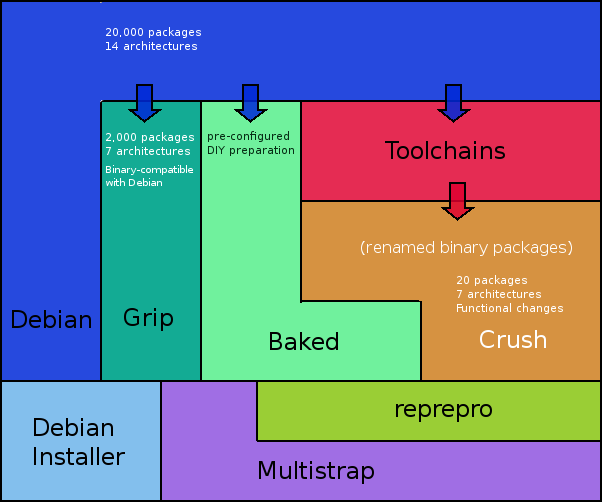
\includegraphics[width=\textwidth]{afbeeldingen/emdebian_soorten}
	\caption{Verschillende soorten van Emdebian en de respectievelijke installatiemogelijkheden}
	\label{fig:emdebian:flavours}
	\legend{(\url{www.emdebian.org}, 2011)}
\end{figure}

Voor de prototype kiosk zullen we gebruik maken van Emdebian Grip, omdat we zo een klein besturingssysteem bekomen maar toch niet te veel flexibiliteit verliezen: als we een pakket nodig hebben dat zich niet in de Emdebian repositories bevindt, kunnen we dat gewoon afhalen van de officiële Debian servers. Dit is vooral interessant omdat we zo applicaties en pakketten kunnen compileren op het toestel zelf, want de Emdebian repositories bevatten niet zoveel development packages. Het alternatief zou bestaan uit het opzettne van een \emph{cross-development environment} op een andere computer, wat vrij veel werk is.
Eenmaal de ontwikkeling van de nodige pakketten voltooid is, kunnen we voor de overige devices gerust gebruik maken van Emdebian Crush of zelfs Baked, aangezien we dan gewoon de pakketten die we reeds op de prototype kiosk gecompileerd hebben moeten installeren.

Zoals figuur \ref{fig:emdebian:flavours} duidelijk maakt kunnen we de verschillende Emdebian basissystemen op verschillende manieren aanmaken. Aangezien we in eerste instantie gebruik zullen maken van Emdebian Grip maar later eventueel wel willen kunnen overschakelen naar Emdebian Crush, zullen we moeten gebruik maken van \code{multistrap} (of zijn voorganger \code{debootstrap}) om het basissysteem samen te stellen. Om multistrap te gebruiken moeten we een configuratiebestand voorzien dat informatie bevat over de pakketten die geïnstalleerd moeten worden. Multistrap zal dit bestand inlezen, alle afhankelijkheden oplossen, en een basissysteem met al deze pakketten genereren.

Maar enkel een basissysteem met de nodige pakketten volstaat niet, we moeten nog verschillende aspecten van het systeem configureren. Daarbij denken we aan netwerkinstellingen, de hostname, welke terminals actief moeten zijn, en welke modules moeten ingeladen worden. Ook kunnen we het resulterende bestandssysteem niet zomaar op een geheugenkaart plaatsen: de partities moeten zodanig aangemaakt zijn dat we vanuit de bootloader exact kunnen verwijzen naar de geheugenadressen van relevante bestanden, \code{uImage} en \code{uInitrd}.

Het is wellicht duidelijk dat dit allemaal geen eenvoudig klusje is. Om zoveel mogelijk te automatiseren en zo menselijke fouten te vermijden, hebben we alle taken beschreven in deze paragraaf gebundeld in \makeurl{https://github.com/MIRAvzw/adastra3-scripts/tree/master/rootfs}{een aantal scripts} die aan de hand van enkele intuïtieve configuratiebestanden het basissysteem volledig autonoom samenstellen.

\subsection{Repository}
\label{kiosk:deployment:besturingssysteem:repository}

Een van de sterktes van Debian is zijn krachtig pakketbeheersysteem. Aangezien we libraries en applicaties gebruiken die zich niet in de standaard Debian repositories bevinden (zoals de kioskapplicatie zelf), moeten we zelf voorzien in een repository met die pakketten in. Hoewel dit niet echt vereist is (zo is het mogelijk om de libraries en applicaties buiten het pakketbeheersysteem om te installeren), heeft dit twee grote voordelen: we kunnen er eenvoudig de software op alle kiosken mee updaten, en het laat toe om het genereren van een volwaardig besturingssysteem volledig te automatiseren met de scripts die we geschreven hebben voor het genereren van het basissysteem.

Vooraleer we een repository kunnen maken, moeten we de code van alle benodigde projecten zodanig verpakken dat de Debian package manager er mee overweg kan. Conversie van een codebase gebeurt met de \code{dpkg-buildpackage} tool, die de code compileert en in een pakketbestand giet aan de hand van een aantal specifieke configuratiebestanden. Zo bevat het \code{control} bestand (zoals er een te zien is in fragment \ref{lst:debian:rules}) essentiële informatie over het pakket: naam, beschrijving, versie, afhankelijkheden, \ldots Een ander belangrijk bestand is het \code{rules} bestand, dat voorschrijft hoe het project geconfigureerd en gecompileerd moet worden. Voor de volledige lijst aan bestanden verwijzen we naar de \makeurl{http://www.debian.org/doc/debian-policy/ch-source.html}{Debian Policy Manual}.

\begin{lstlisting}[float, caption=Debian control packaging bestand., label=lst:debian:rules]
Source: aa3client
Maintainer: Tim Besard <tim.besard@gmail.com>
Homepage: https://sites.google.com/site/miraadastraiii/
Priority: extra
Build-Depends: debhelper (>= 7.0.50~),
               qt4-qmake, libqt4-dev, libbrisa-dev,
               liblog4qt-dev, libsvnqt2-dev, pkg-config
Standards-Version: 3.8.4
Vcs-Git: git://github.com/MIRAvzw/adastra3-client.git
Vcs-Browser: https://github.com/MIRAvzw/adastra3-client

Package: aa3client
Section: lib
Architecture: any
Depends: libqt4-core, libqt4-gui, libqt4-webkit,
         libbrisa, liblog4qt, libsvnqt2,
         ${misc:Depends}, ${shlibs:Depends}
Description: Ad-Astra III client application

Package: aa3client-dbg
Section: libdevel
Architecture: any
Depends: libbrisa (= ${binary:Version}), ${misc:Depends}
Description: Ad-Astra III client application
             (debug symbols)
\end{lstlisting}

Om de gegenereerde pakketten toegankelijk te maken voor het Debian pakketbeheersysteem, moeten we ze onderbrengen in een repository. Dit is eigenlijk niet meer dan een heel exacte bestandshiërarchie, uitgebreid met enkele metabestanden die informatie bevatten over de aanwezige pakketten. Er bestaan verschillende tools om een repository aan te maken, waarbij er enorme verschillen zijn in de mogelijkheden. Omdat onze repository slechts enkele pakketten gaat bevatten, en louter voor intern gebruik dient, kiezen we voor een van de meest eenvoudige tools: \code{apt-ftparchive}. Deze applicatie doet eigenlijk niet veel meer dan het aanmaken van de nodige metabestanden, gebaseerd op een configuratiebestand met alle instellingen erin. Het aanmaken van de exacte bestandshiërarchie met de pakketten op de juiste plaats is de verantwoordelijkheid van de gebruiker, \code{apt-ftparchive} maakt enkel de nodige metabestanden aan. Fragment \ref{lst:debian:repo} illustreert de bestandshiërarchie van een repository met een enkel pakket in.

\begin{lstlisting}[float, caption=Bestandshiërarchie in een Debian repository., label=lst:debian:repo]
debian
|-- dists
|   +-- squeeze
|       |-- Release
|       |-- dev
|       |   |-- binary-armel
|       |   |   |-- Packages
|       |   +-- source
|       |       |-- Packages
|       |       +-- Sources
|       +-- main
|           |-- binary-armel
|           |   |-- Packages
|           +-- source
|               |-- Packages
|               +-- Sources
+-- pool
    |-- dev
    |   |-- aa3client-dbg_0.1-1_armel.deb
    +-- main
        |-- aa3client_0.1-1.dsc
        |-- aa3client_0.1-1.tar.gz
        |-- aa3client_0.1-1_armel.changes
        +-- aa3client_0.1-1_armel.deb
\end{lstlisting}

Tenslotte moeten we de repository nog publiceren, wat kan via een aantal protocollen. We hebben gekozen voor het \ac{ftp}, omdat dergelijke functionaliteit reeds ingebouwd is in het besturingssysteem van de Synology DS207+, de \ac{nas} die we gebruiken als server.

Een repository samenstellen met al zijn pakketten erin is opnieuw een vrij complex en foutgevoelig proces. Daarom hebben we weer zoveel mogelijk proberen te automatiseren met \makeurl{https://github.com/MIRAvzw/adastra3-scripts/tree/master/packages}{een aantal scripts}, die volledig autonoom broncode van projecten kunnen ophalen, er pakketten van maken, ze bundelen in een repository, en finaal die repository deployen op een externe server.

\section{Versioning}
\label{kiosk:deployment:versioning}

Ook voor de kioskapplicatie maken we gebruik van het Git versioning systeem; wat we in sectie \ref{server:deployment:versioning} beschreven hebben is dus hier ook van toepassing.

\section{Compilatie}
\label{kiosk:deployment:compilatie}

Om de software te compileren maken we gebruik van de tools die het Qt framework daartoe biedt. De belangrijkste daarvan is \code{qmake}, een applicatie die het genereren van een \code{Makefile} automatiseert. Dit is vooral interessant omdat, zoals hierboven vermeld, bronbestanden die gebruik maken van Qt-macro's eerst moeten voorverwerkt worden door de \ac{moc} preprocessor. Door gebruik te maken van \code{qmake} moeten we dit niet langer manueel doen: \code{qmake} detecteert welke bestanden eerst moeten verwerkt worden door de preprocessor, en genereert een \code{Makefile} waarbij dit dan ook eerst gebeurt.

Ook hebben we tijdens de ontwikkeling van de applicatie gebruik gemaakt van \makeurl{http://clang.llvm.org/}{Clang}, een moderne compiler voor C en C++. Hoewel deze vrij jonge compiler nog niet op hetzelfde niveau staat als de \ac{gcc}, is het op enkele vlakken veel beter dan \ac{gcc}. Zo is er zeer veel aandacht besteed aan het error reporting subsysteem, waardoor de foutmeldingen die Clang genereert vaak een pak behulpzamer zijn dan wat \ac{gcc} in eenzelfde situatie zou laten weten. Toch worden de uiteindelijke executables gegenereerd met \ac{gcc}, omdat die op vlak van optimalisaties (zowel op vlak van snelheid als grootte) nog steeds de beste keuze is.

Tenslotte is het nog het vermelden waard dat alle libraries die we gebruiken dynamisch gelinkt worden met de finale executable. Dit betekent dat de libraries op het systeem aanwezig moeten zijn, en niet met de applicatie gebundeld worden. Bij de serverapplicatie hebben we dit net anders gedaan, zoals beschreven in sectie \ref{server:deployment:compilatie} hebben we daar alles gebundeld tot een enkel monilitisch geheel. De redenering hierachter is tweeledig. Enerzijds is een kiosk veel statischer: eenmaal we het besturingssysteem samengesteld hebben en er alle nodige applicaties op geïnstalleerd hebben zullen we er lange tijd af blijven. Bij de server is dat anders, niet alleen kunnen en zullen we vaker van hardware veranderen (waarbij vervolgens het besturingssysteem vernieuwd moet worden), ook kunnen we het ons bij een genetwerkte server uit veiligheidsoverwegingen niet veroorloven om jaren aan een stuk dezelfde software te gebruiken. Anderzijds verschillende ook de beschikbare voorzieningen om code in gedeelde bibliotheken af te zonderen: bij C++ code is dit bijvoorbeeld heel eenvoudig dankzij de ingebouwde en sterk geïntegreerde \emph{dynamic linker}. Voor Java applicaties is dit niet het geval: archieven kunnen op arbitraire plaatsen terechtkomen en er zijn geen algemeen aanvaarde mechanismen om die locaties eenduidig te ontdekken en op te vragen bij het opstarten van een applicatie.

\part{Inputmodule}
\label{inputmodule}

\chapter{Hardware}
\label{inputmodule:hardware}

Zoals uit de doeken gedaan in deel \ref{ontwerp}, zullen we voor de module gebruik maken van een AVR microcontroller met daarop de V-USB firmware om low-speed datacommunicatie te verwezenlijken met minimale periferie.

\section{Microcontroller}
\label{inputmodule:hardware:microcontroller}

Door het gebruik van de V-USB bibliotheek moeten we ons beperken tot AVR microcontrollers, maar binnen die familie is het aanbod nog altijd zeer groot. Om een goede selectie te maken, moeten we logischerwijs rekening houden met de eisen die de V-USB bibliotheek stelt:
\begin{itemize}
\item Flash: tenminste 2 kB;
\item RAM: tenminste 128 bytes;
\item Kloksnelheid: 12.8 of 16.5 MHz bij gebruik van een interne oscillator, en ook 12, 15, 16 of 20 MHz indien we gebruik maken van een extern kristal\footnote{Dit omdat enkel de 12.8 en 16.5 MHz frequenties een deviatie van 1\% toelaten, en het bij de interne oscillator onmogelijk is om een heel precieze afstelling te bekomen.};
\item Poorten: exact 2, beide met een interruptlijn.
\end{itemize}

We willen echter ook een uitbreidbare module realiseren. Momenteel hebben we slechts 4 knoppen aan te sluiten, maar mogelijks worden dit er later meer. Daarom zullen we de ruimte laten voor drie extra knoppen, wat we eenvoudig kunnen realiseren met slechts 4 poorten door het signaal te multiplexen. Als we tenslotte overlappingen negeren, volstaat het zelfs om maar 3 poorten te gebruiken.

Tenslotte zou het ook interessant zijn moest de microcontroller voorzien van \ac{isp} headers, waardoor de firmware van de module achteraf nog kan vernieuwd worden zonder daarvoor de microcontroller te moeten verwijderen uit de module. Indien we het echter mogelijk willen maken om de chip te herprogrammeren via \ac{isp}, kunnen we geen gebruik maken van \ac{hvsp} (waarvoor de chip fysiek moet geplaatst in een \ac{hvsp} programmer moet geplaatst worden). \ac{hvsp} is een speciale methode om een microcontroller te programmeren, waarbij het mogelijk is om voordien ingestelde \emph{fuses} opnieuw in te stellen. Zo is er bijvoorbeeld de fuse die de \code{RESET}-poort (aanwezig op elke AVR microcontroller) configureert als een reguliere input/output poort. Deze fuse kan initieel wel ingesteld worden via \ac{isp}, maar heeft als consequentie dat de chip nadien niet meer kan geherprogrammeerd worden, tenzij door gebruik te maken van \ac{hvsp} waarmee de fuse in kwestie opnieuw ingesteld kan worden. Hierdoor is het dus onmogelijk om de \code{RESET}-poort te gebruiken als reguliere poort.

Een microcontroller die voldoet aan deze eisen, is de \strong{AtTiny45}. Deze heeft de volgende relevante specificaties:
\begin{itemize}
\item Flash: 4 kB;
\item RAM: 256 bytes;
\item EEPROM: 256 bytes;
\item ISP: aanwezig;
\item Kloksnelheid: 10 MHz voor de low-voltage versie, en tot 20 MHz voor de reguliere versie;
\item Interne oscillator: gekalibreerd voor 8 MHz;
\item Voedingsspanning: 1.8-5.5 volt voor de low-voltage versie, en 2.7-5.5 volt voor de reguliere versie.
\end{itemize}

\subsection{Kloksnelheid}

Om het aantal componenten te minimaliseren, zouden we de module graag realiseren zonder gebruik te maken van een externe oscillator. De interne oscillator is echter enkel gekalibreerd om op 8 MHz te werken, wat niet bruikbaar is in combinatie met V-USB. Om toch een bruikbare frequentie te bekomen, maken we gebruik van een kalibratiemechanisme dat we vonden in het \makeurl{http://www.obdev.at/products/vusb/easylogger.html}{EasyLogger} voorbeeldproject.

De eerste stap bestaat uit het kalibreren van de interne oscillator tot een frequentie van 8.25 MHz, dit door te vergelijken met binnenkomende \ac{usb} frames en binair te zoeken naar een optimale waarde voor het \code{OSCCAL} oscillator kalibratieregister. Hierdoor zal de \ac{pll} clock, steeds gelijk aan een achtvoudige versnelling van de interne oscillator, ingesteld worden op 66 MHz. Indien we tenslotte de \code{CLKSEL} fuse bij het programmeren instellen op $0001$ zal de systeemklok gelijk ingesteld worden aan de \ac{pll} clock gedeeld door 4, wat overeen komt met 16.5 MHz, een frequentie die we kunnen gebruiken in combinatie met de V-USB code.

\subsection{Voeding}

Aangezien de kloksnelheid waarop onze microcontroller zal draaien, 16.5 MHz, groter is dan 10 MHz, zullen we geen gebruik kunnen maken van de low-voltage versie. Meer nog: om een kloksnelheid groter dan 10 MHz te bekomen, zal de voedingsspanning zelfs tussen de 4.5 en 5.5 volt moeten bedragen. Op het eerste zicht vormt dit geen probleem, we kunnen immers de \ac{usb} voedingslijn (mits ontkoppeling) direct gebruiken om de microcontroller te voeden. Maar zoals uit de volgende paragraaf zal blijken, zou het zo ook zijn voordelen kennen moesten we de microcontroller kunnen voeden met een lagere spanning.

Natuurlijk zullen we ook de voedingsspanning ontkoppelen, en dit op twee vlakken. Om de hoogfrequente schakelpieken van de digitale microcontroller af te vlakken, plaatsen we een 100 nanofarad condensator tussen de voedingslijn en de grondplaat. Het valt op te merken dat we die condensator zo dicht mogelijk tegen de voedingspin van de microcontroller willen plaatsen, dit om parasitaire capaciteiten te vermijden. Vervolgens willen we ook eventuele onregelmatigheden afvlakken (hetzij van de spanningsbron uit, hetzij veroorzaakt door een plotse toename in verbruik), waarvoor we een 10 microfarad condensator plaatsen aan de kant van de \ac{usb} connector. De waarde van 10 microfarad is niet uit de lucht gegrepen: ze is relatief hoog om de typisch laagfrequentere pieken die een spanningsbron genereert af te vlakken, en tegelijk is het ook het maximum dat de \ac{usb} specificatie toelaat \citep{usbnutshell}.

\begin{figure}
	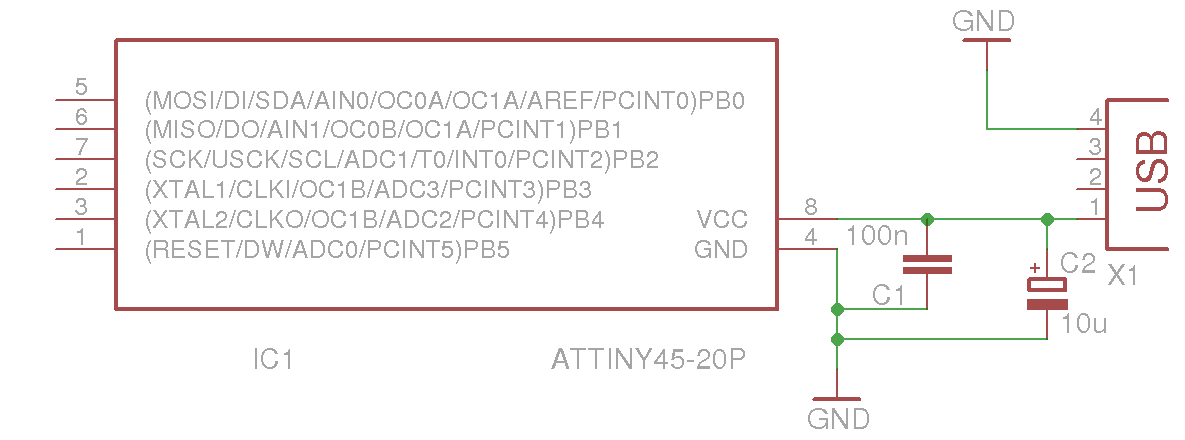
\includegraphics[width=\textwidth]{afbeeldingen/inputmodule_voeding}
	\caption{Voedingscircuit}
\end{figure}

\subsection{Signalen}

\ac{usb} datacommunicatie verloopt steeds over een \emph{twisted-pair}, op een differentiële manier. Dit betekent dat een signaalbit afgeleid wordt uit het potentiaalverschil tussen de twee signaaldragers, en dat die binnen een \ac{usb}-kabel steeds gedraaid (\emph{twisted}) zijn. Het voordeel van het draaien is dat eventuele ruis grotendeels evenredig verdeeld is over beide kabels, waardoor het potentiaalverschil tussen beide vaak onveranderd blijft. Hierdoor is differentiële dataoverdracht over een twisted-pair veel beter bestand tegen elektromagnetische ruis.

Eerst en vooral zorgen we voor een stroombeperking op de signaaldragers. Hiertoe zullen we tussen de signaalpin en de \ac{usb} connector een weerstand van 68 ohm plaatsen, die ervoor zorgen dat er nooit meer dan 50 milliampères zal vloeien.

De specifieke elektrische kenmerken van de implementatie in het \ac{usb} protocol zijn vervelend voor gebruik in combinatie met de meeste digitale componenten. Zo wordt een hoog signaal gekenmerkt door een differentieel signaal van 2.8 tot 3.6 volt, terwijl voor een laag signaal 0 tot 0.3 volt te detecteren valt. Voor toekomende signalen (het twisted-pair is immers half-duplex) vormen deze waarden geen probleem: de meeste microcontrollers, waaronder de gebruikte AtTiny45, herkennen een signaal van 3.3 volt als een hoog signaal (hoewel de specificatie slechts een bereik vastlegt, sturen de meeste hosts exact 3.3 volt) . Wat wel een probleem vormt, zijn de uitgaande signalen. Aangezien onze microcontroller gevoed wordt door 5 volt, kennen de signalen tevens een spanning van 5 volt, wat ruimschoots buiten het opgelegde bereik valt.

Een mogelijke oplossing bestaat eruit de \strong{voedingsspanning van de microcontroller te verlagen} tot 3.6 volt. Aangezien de spanning die de microcontroller gebruikt op de signaalpinnen min of meer gelijk is aan de voedingsspanning, en de AtTiny45 genoeg heeft aan slechts 1.8 tot 2.7 volt (afhankelijk van de uitvoering), zou dit het probleem direct oplossen. Er zou enkel nood zijn aan een spanningsregulator om de voedingsspanning te reduceren tot 3.6 volt, wat dan wel een \emph{low-drop} regulator zou moeten zijn (omdat gewone regulators meestal een initiële drop van 2 volt kennen). Een minder robuust alternatief vervangt deze regulator door twee diodes, waardoor een voltage drop van 1.2 tot 1.4 volt bekomen wordt.
Jammer genoeg kunnen we geen van deze oplossingen gebruiken, omdat de microcontroller op 16.5 MHz zal draaien waarvoor we een voedingsspanning tussen de 4.5 en 5 volt nodig hebben.

Een alternatief bestaat eruit om het \textbf{spanningsniveau van de signaalpinnen te reguleren}. Hiertoe raadt de \makeurl{http://vusb.wikidot.com/hardware}{V-USB wiki} bijvoorbeeld aan om gebruik te maken van 3.6 volt zenerdioden. Zenerdioden hebben immers de eigenschap dat ze ook in sperstand kunnen geleiden, wanneer de zenerspanning bereikt is. Daarbij is de spanningsval over de diode dan ook relatief constant, los van de spanning die er aan gelegd wordt. Meer concreet houdt dit in dat indien we de signaalpinnen via een zenerdiode in sper verbinden met de grondplaat, de spanning van het signaal gereduceerd wordt tot 3.6 volt. Deze opzet kent echter ook enkele problemen. Zo kan het moeilijk zijn om de exacte combinatie van parameters vast te leggen, zenerdiodes komen immers in soorten en maten. Een ander nadeel zijn de hoge stromen veroorzaakt door de zenerdiode. Wanneer de diode immers een hoog 5 volt signaal reduceert tot 3.6 volt, zal de overige 1.4 volt over de 68 ohm weerstanden tussen de microcontroller en de \ac{usb} host komen te staan, wat zorgt voor liefst 20 milliampères over de signaaldrager.

Tenslotte moeten we nog voorzien in een \emph{setting weerstand} die een spanning plaatst op de negatieve signaaldrager. Deze pull-up weerstand maakt aan de \ac{usb} host duidelijk dat er een \ac{usb} 1.1 toestel aangesloten is (weliswaar actief in \emph{low speed} modus). Voor een 5 volt lijn kan dit gerealiseerd worden met een 1k8 of 2k2 ohm weerstand.

\begin{figure}
	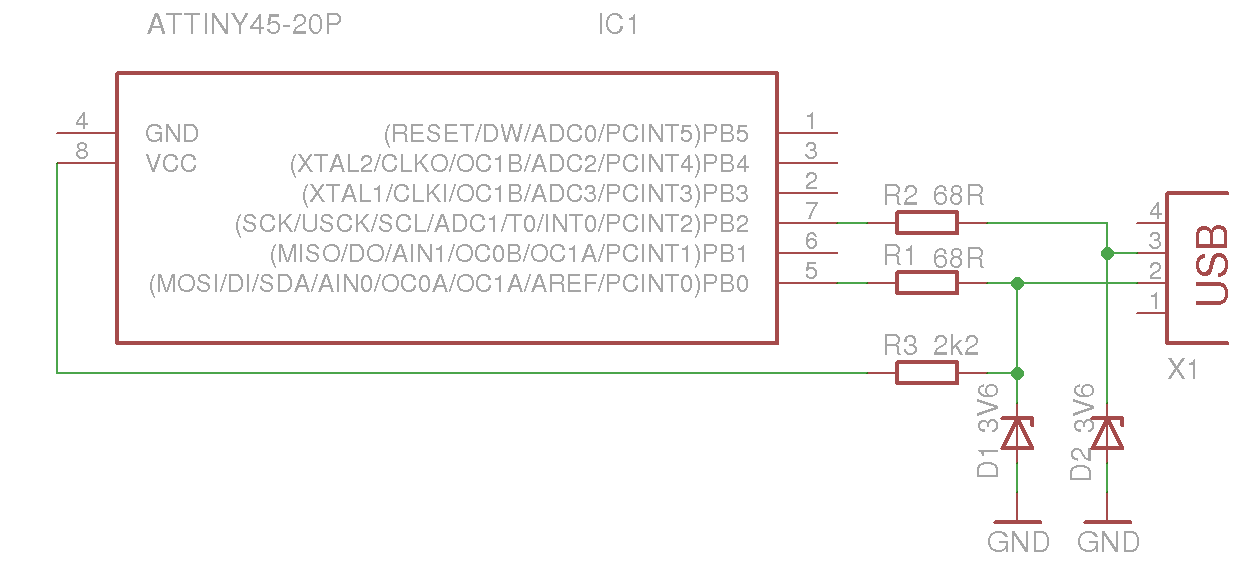
\includegraphics[width=\textwidth]{afbeeldingen/inputmodule_signaal}
	\caption{Signaalconversie}
\end{figure}

\subsection{\acs{isp}}

Het invoegen van een \ac{isp} header is niet veel werk: we dienen gewoon te voorzien in een connector, en de pinnen ervan correct doorverbinden met de juiste pinnen van de microcontroller.

\begin{figure}
	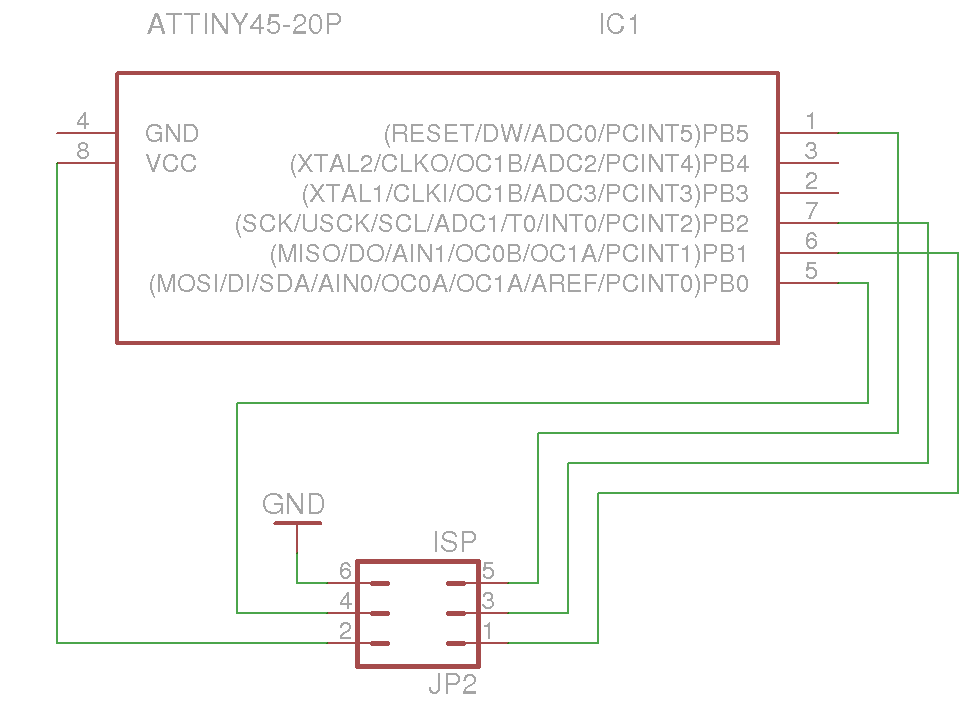
\includegraphics[width=\textwidth]{afbeeldingen/inputmodule_isp}
	\caption{\acs{isp} connector}
\end{figure}

\section{Schakelaars}
\label{inputmodule:hardware:schakelaars}

De schakelaars bevinden zich fysiek niet op de inputmodule, maar zijn reeds ingebouwd in de bestaande kasten. Daarom zullen we een systeem moeten bedenken om de bestaande schakelaars op een handige manier op de module aan te sluiten. Tevens moeten we de knoppen zodanig verbinden dat er uitbreidingsmogelijkheden zijn.

Om de bestaande schakelaars op een eenvoudige manier aan te sluiten, zullen we de inputmodule voorzien van een connector waarop we eenvoudig knoppen kunnen op aansluiten. De meest robuuste oplossing hierbij is een connector die vastklikt op de module, waardoor die niet per toeval kan loskomen. Dergelijke connectors zijn echter vrij specifiek, en vereisen per aan te sluiten schakelaar een element op de printplaat. Een alternatief, dat als voordeel heeft dat het geen speciale connector aan de kant van de knoppen vereist, zijn vijs-connectors. Hierbij worden de losse draden van de knoppen via een vijsaansluiting op de printplaat bevestigd. Hoewel dit al een betere oplossing is, vereist het nog altijd een connector op de printplaat voor elke knop, en neemt het vast- en losvijzen van de kabels ook meer tijd in beslag dan het aansluiten van een eenvoudige connector. Daarom hebben we gekozen voor de alombekende \emph{jumpers}. Deze makkelijk te vinden connectors kunnen eenvoudig aan het kabelpaar van de knoppen bevestigd worden door middel van een krimptang. Aan de kant van de printplaat is het ook een eenvoudigere oplossing, daar het mogelijk is de aansluitingen voor alle schakelaars door middel van een enkel blok jumpers te realiseren. Het enige nadeel is dat een aangesloten connectors niet zo vast zitten: bij gebrek aan weerhaak of ander systeem kan de kabel relatief gemakkelijk loskomen.

Om de aansluitingen op de printplaat eenvoudig te houden, zullen we werken met een \emph{active-low} mechanisme: een knop zal, wanneer ingedrukt, bepaalde signaallijnen doorverbinden met de elektrische grond. Om er voor te zorgen dat er een hoog signaal gemeten wordt wanneer er geen verbinding is met de elektrische grond, maken we gebruik van de interne pull-up die beschikbaar is voor elke poortpin: dit is een weerstand tussen de $20$ en $50$ kilo-ohm die de poortpin intern doorverbindt met de positieve voedingslijn. Hierdoor zal bij afwezigheid van een externe verbinding de spanning op de poortpin gelijk zijn aan de voedingsspanning, wat gedetecteerd wordt als een hoog signaal. Wanneer we echter de poortpin zullen doorverbinden naar de elektrische grond, zal deze pull-up weerstand zorgen voor een stroom tussen de $0.1$ en $0.25$ milliampères.

Er is echter een bijkomend probleem: we hebben maar 3 poortpinnen tot onze beschikking, waardoor het niet mogelijk is elke knop door te verbinden met een eigen poortpin. De eenvoudige oplossing hierbij is het gebruik van een multiplexer: 2 select-lijnen en 1 datalijn maakt het mogelijk om 4 schakelaars uit te lezen. We willen echter meer knoppen kunnen aansluiten, zonder daarbij extra poortpinnen nodig te hebben. Daarom zullen we zelf het signaal multiplexen, waarbij we meer schakelaars kunnen toelaten door geen gebruik te maken van een selectiemechanisme, maar de signalen direct door te linken naar de poortpinnen. Het nadeel aan deze opzet is dat de signalen kunnen overlappen, zo zullen we bij het indrukken van meerdere knoppen tegelijkertijd niet kunnen uitmaken welke knoppen juist ingedrukt zijn.

De realisatie van een dergelijke multiplexer lijkt eenvoudig, maar er is een belangrijk detail dat we moeten opmerken. Aangezien de verschillende poortpinnen verbonden zijn met verschillende knoppen, kan er bij het indrukken van een enkele schakelaar stroom terugvloeien via de contactpunten van diens signaallijnen met andere knoppen van een totaal ongerelateerde poortpin. Om dit te vermijden moeten we overal waar er twee signaallijnen met elkaar verbonden zijn, een diode plaatsen zodat er geen stroom kan terugvloeien naar een vorig verbindingspunt. Hiervoor hebben we een reguliere diode nodig, waarbij geen speciale eisen gesteld worden. Daarom kiezen we voor de 1N4148, een populaire diode die vaak gebruikt wordt voor het schakelen van digitale signalen. Zoals we kunnen opzoeken in het stroom-spanningsdiagram van deze diode, zorgt ze bij een stroom tussen $0.1$ en $0.25$ milliampères (gegenereerd door de pull-up weerstand binnen de microcontroller) voor een spanningsval van $0.5$ volt.

\begin{figure}
	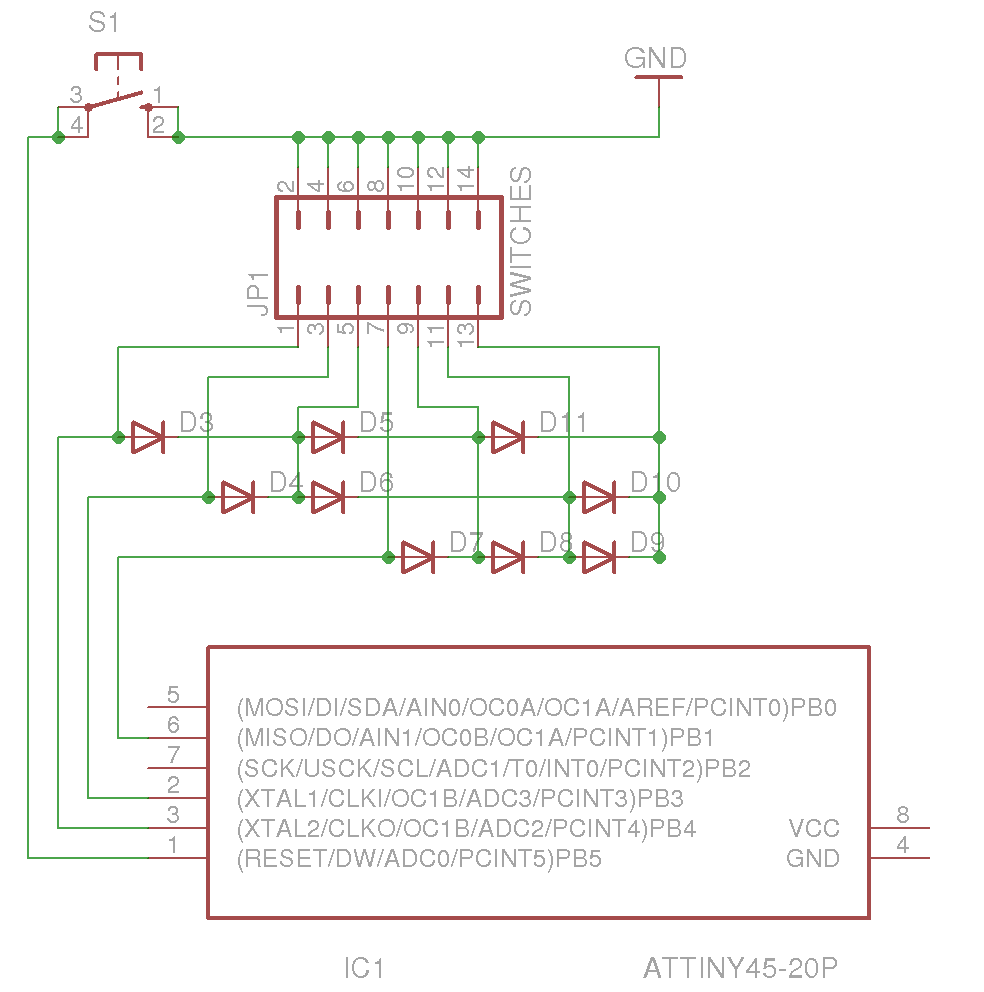
\includegraphics[width=\textwidth]{afbeeldingen/inputmodule_schakelaars}
	\caption{Circuit en connector voor schakelaars}
\end{figure}

\section{Productie}
\label{inputmodule:hardware:productie}

De laatste stap bestaat eruit om het ontworpen schema te realiseren en een fysieke printplaat te laten maken, ofte een \ac{pcb}. Hierbij moeten we manueel een fysieke layout aanmaken en baantjes trekken waar er stroom moet kunnen vloeien. De plaatsing van die componenten is echter niet louter willekeurig. Zo is het bijvoorbeeld interessant om de componenten efficiënt te plaatsen zodat de uiteindelijke printplaat zo klein mogelijk is. Maar er zijn ook andere zaken waarmee we moeten rekening houden. Zo is er bijvoorbeeld de kwestie van plaatsing van de ontkoppelingscondesatoren: die worden best zo dicht mogelijk bij de bron van de spanningsoscillaties geplaatst.

Eerst zijn we op zoek gegaan naar een fabrikant die voor een aanvaardbaar tarief een voldoende gesofisticeerde printplaat kan produceren. De mogelijkheden zijn eens te meer zeer uitgebreid, maar na een uitgebreide vergelijking zijn we terechtgekomen bij \makeurl{http://www.eurocircuits.com/}{Eurocircuits}, een Europees bedrijf met verschillende vestigingen, waaronder België. Hoewel de verschillen tussen andere fabrikanten niet al te groot zijn, heeft de combinatie van een competitieve prijs, beperkte verzendkosten, en verschillende positieve kritieken ons ertoe overtuigd om voor de diensten van Eurocircuits te kiezen.

Dan hebben we een gekeken naar de eisen en mogelijkheden die het goedkoopste van de productietypes te vinden bij Eurocircuits - de standard pool - biedt. De \makeurl{http://www.eurocircuits.com/images/stories/ec09/ec-standard-pool-overview-english-1-2010-v3.pdf}{volledige lijst} is te uitgebreid om hier te vermelden, daarom halen we enkel de belangrijkste elementen aan:
\begin{itemize}
\item Maximaal 8 layers;
\item Top- en bottom solder mask;
\item Top- en bottom silkscreen.
\end{itemize}
Om de overige eisen, denk maar aan de minimale afstand tussen boorgaten of de minimale breedte van elektrische baantjes, te controleren zullen we gebruik maken van een \ac{dru} bestand. Dergelijke bestanden worden vaak aangeboden door te fabrikant, en laten toe om geautomatiseerd alle eisen te controleren die aan een printplaat gesteld worden.

Om een printplaat of \ac{pcb} te ontwerpen hebben we natuurlijk gepaste software nodig. De meest populaire keuze hierbij is de EAGLE PCB software, ontwikkeld door \makeurl{http://www.cadsoftusa.com/}{CadSoft}, waarschijnlijk omdat er een beperkte variant van de software gratis beschikbaar is. Wegens de populariteit van de tool bestaat er een heel actieve community, waardoor een zeer uitgebreide selectie aan componenten beschikbaar is voor gebruik binnen EAGLE. Ook biedt Eurocircuits enkel \ac{dru} bestanden aan voor de EAGLE software. Het lijkt daarom een verstandige keuze om onze printplaat ook te ontwerpen met EAGLE.

Nu we alle nodige specificaties vergaard hebben en een softwarepakket geselecteerd hebben, kunnen we beginnen aan het produceren van de fysieke layout. Hierbij hebben we ervoor gekozen om een printplaat te maken die bestaat uit twee lagen, namelijk de boven en onderkant. Deze optie is niet veel duurder dan een 1-laags printplaat, en het geeft ons de nodige flexibiliteit om de componenten goed te kunnen plaatsen. Moesten we gekozen hebben voor een 1-laags printplaat dan zou de kost misschien zelfs hoger kunnen liggen door soms onnatuurlijke plaatsing om toch de nodige verbindingen te kunnen realiseren. 

De finale versie van de 2-laags printplaat is te vinden in figuur \ref{fig:printplaat}. Hierbij zijn een aantal zaken waard om te vermelden. Zo is er de plaatsing van de 100 nanofarad condensator die instaat voor het ontkoppelen van de hoogfrequente ruis: aangezien dergelijke ruis veroorzaakt wordt door het schakelen van de transistoren binnen de microcontroller, hebben we de condensator zo dicht mogelijk geplaatst bij de bron van die ruis. Ook hebben we, zoals het de gewoonte is bij het ontwerpen van een schema, de vrije ruimte van elke laag gebruikt om een volledig geleidend vlak te maken. Daarbij zal de fill op de bovenste layer gebruikt worden om de positieve voedingsspanning $Vcc$ te geleiden, en de fill op de onderste layer om de elektronische grond te verdelen. Hoewel dit bij een hoogfrequent-circuit niet zou aan te raden is wegens de parasitaire capaciteiten die gepaard gaan met dergelijke \emph{plane fills}, is dit bij ons relatief laagfrequent schema niet van toepassing.

\begin{figure}
	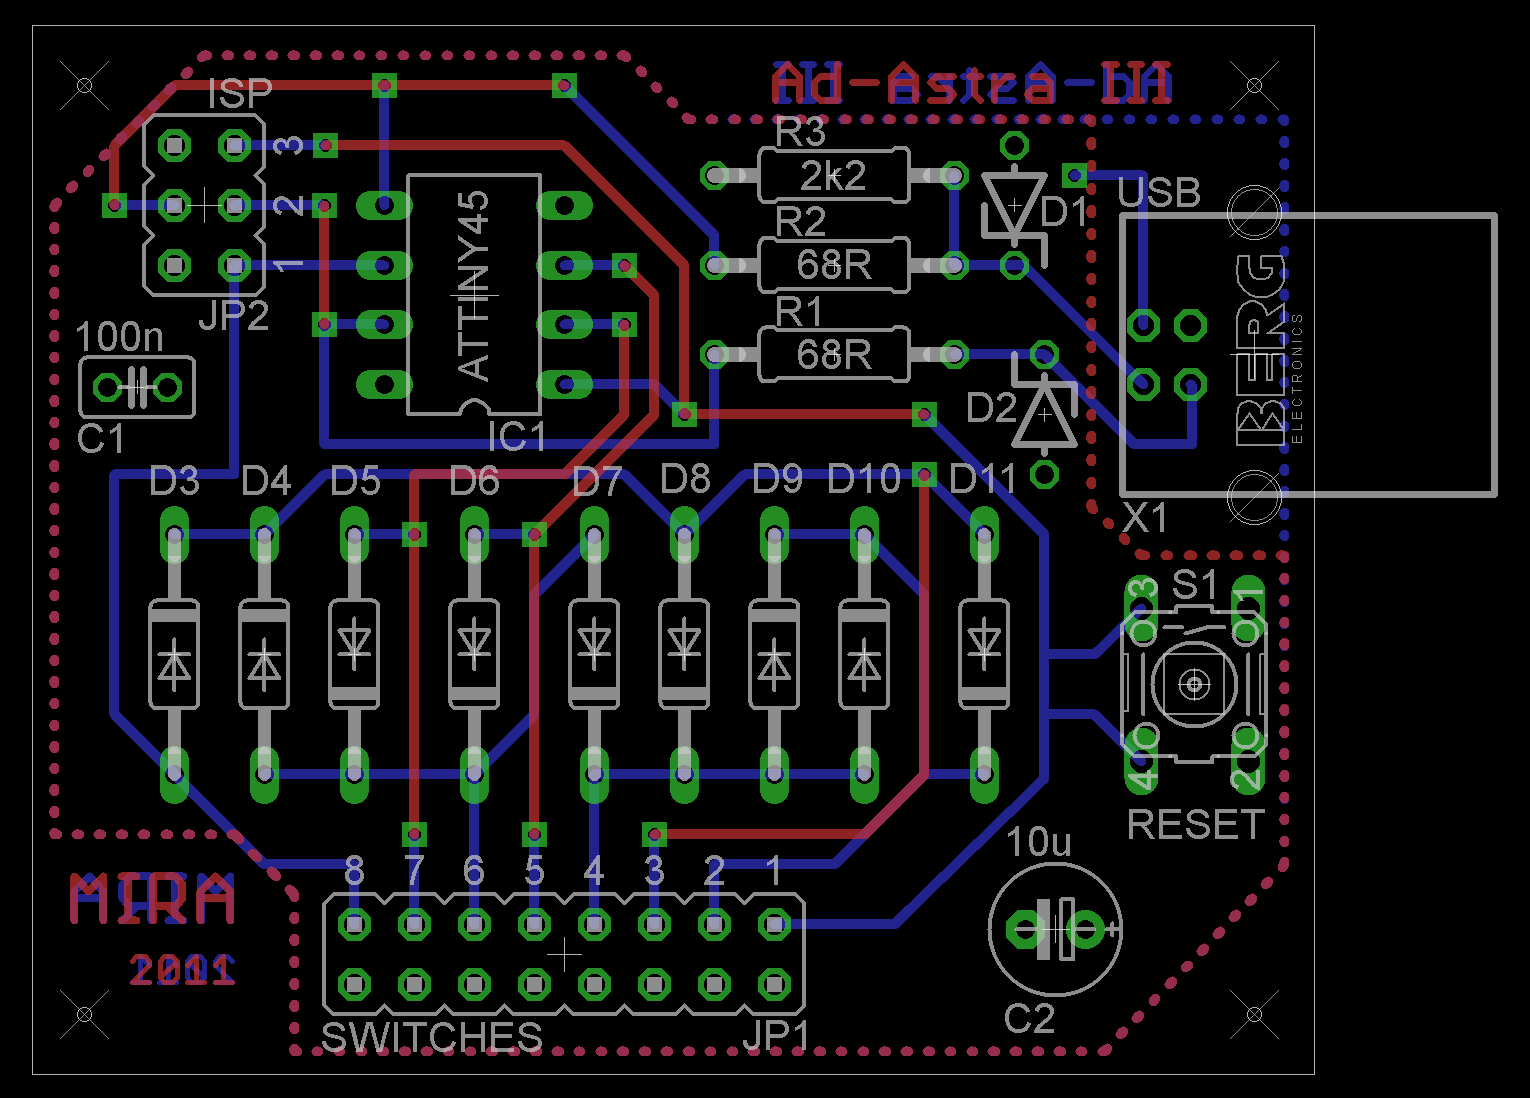
\includegraphics[width=\textwidth]{afbeeldingen/inputmodule_pcb}
	\caption{Finale versie van de printplaat}
	\label{fig:printplaat}
\end{figure}

De laatste stap voor de effectieve productie is de conversie van ons schema naar het bestandsformaat dat vereist is door Eurocircuits. Hoewel dit verschilt van producent tot producent, moeten we meestal voorzien in de volgende bestanden (met het formaat steeds tussen haakjes):
\begin{itemize}
  \item Top copper (Extended Gerber): koper op bovenste laag;
  \item Bottom Copper (Extended Gerber): koper op onderste laag;
  \item Top Silkscreen (Extended Gerber): tekst op bovenste laag;
  \item Top Soldermask (Extended Gerber): plaatsen op bovenste laag die moeten bedekt worden met beschermende laag;
  \item Bottom Soldermask (Extended Gerber): plaatsen op bovenste laag die moeten bedekt worden met beschermende laag;
  \item Drill File (Excellon): waar en hoe er geboord moet worden op de printplaat.
\end{itemize}

Het genereren van deze bestanden kunnen we uitvoeren met Eagle's CAM Processor. Hiertoe hebben we ons gebaseerd op een voorbeeld CAM job van Sparkfun, aangepast aan de specifieke eisen die Eurocircuit stelt. Na het insturen van deze bestanden, selectie van de benodigde materialen en processen, kregen we na enkele weken een afgewerkte printplaat in de bus. Vervolgens zijn we overgegaan tot aankoop van de benodigde componenten, waarna we die er op gesoldeerd hebben om dan eindelijk een afgewerkte print te bekomen zoals te zien in figuur \ref{fig:inputmodule}.

\begin{figure}
	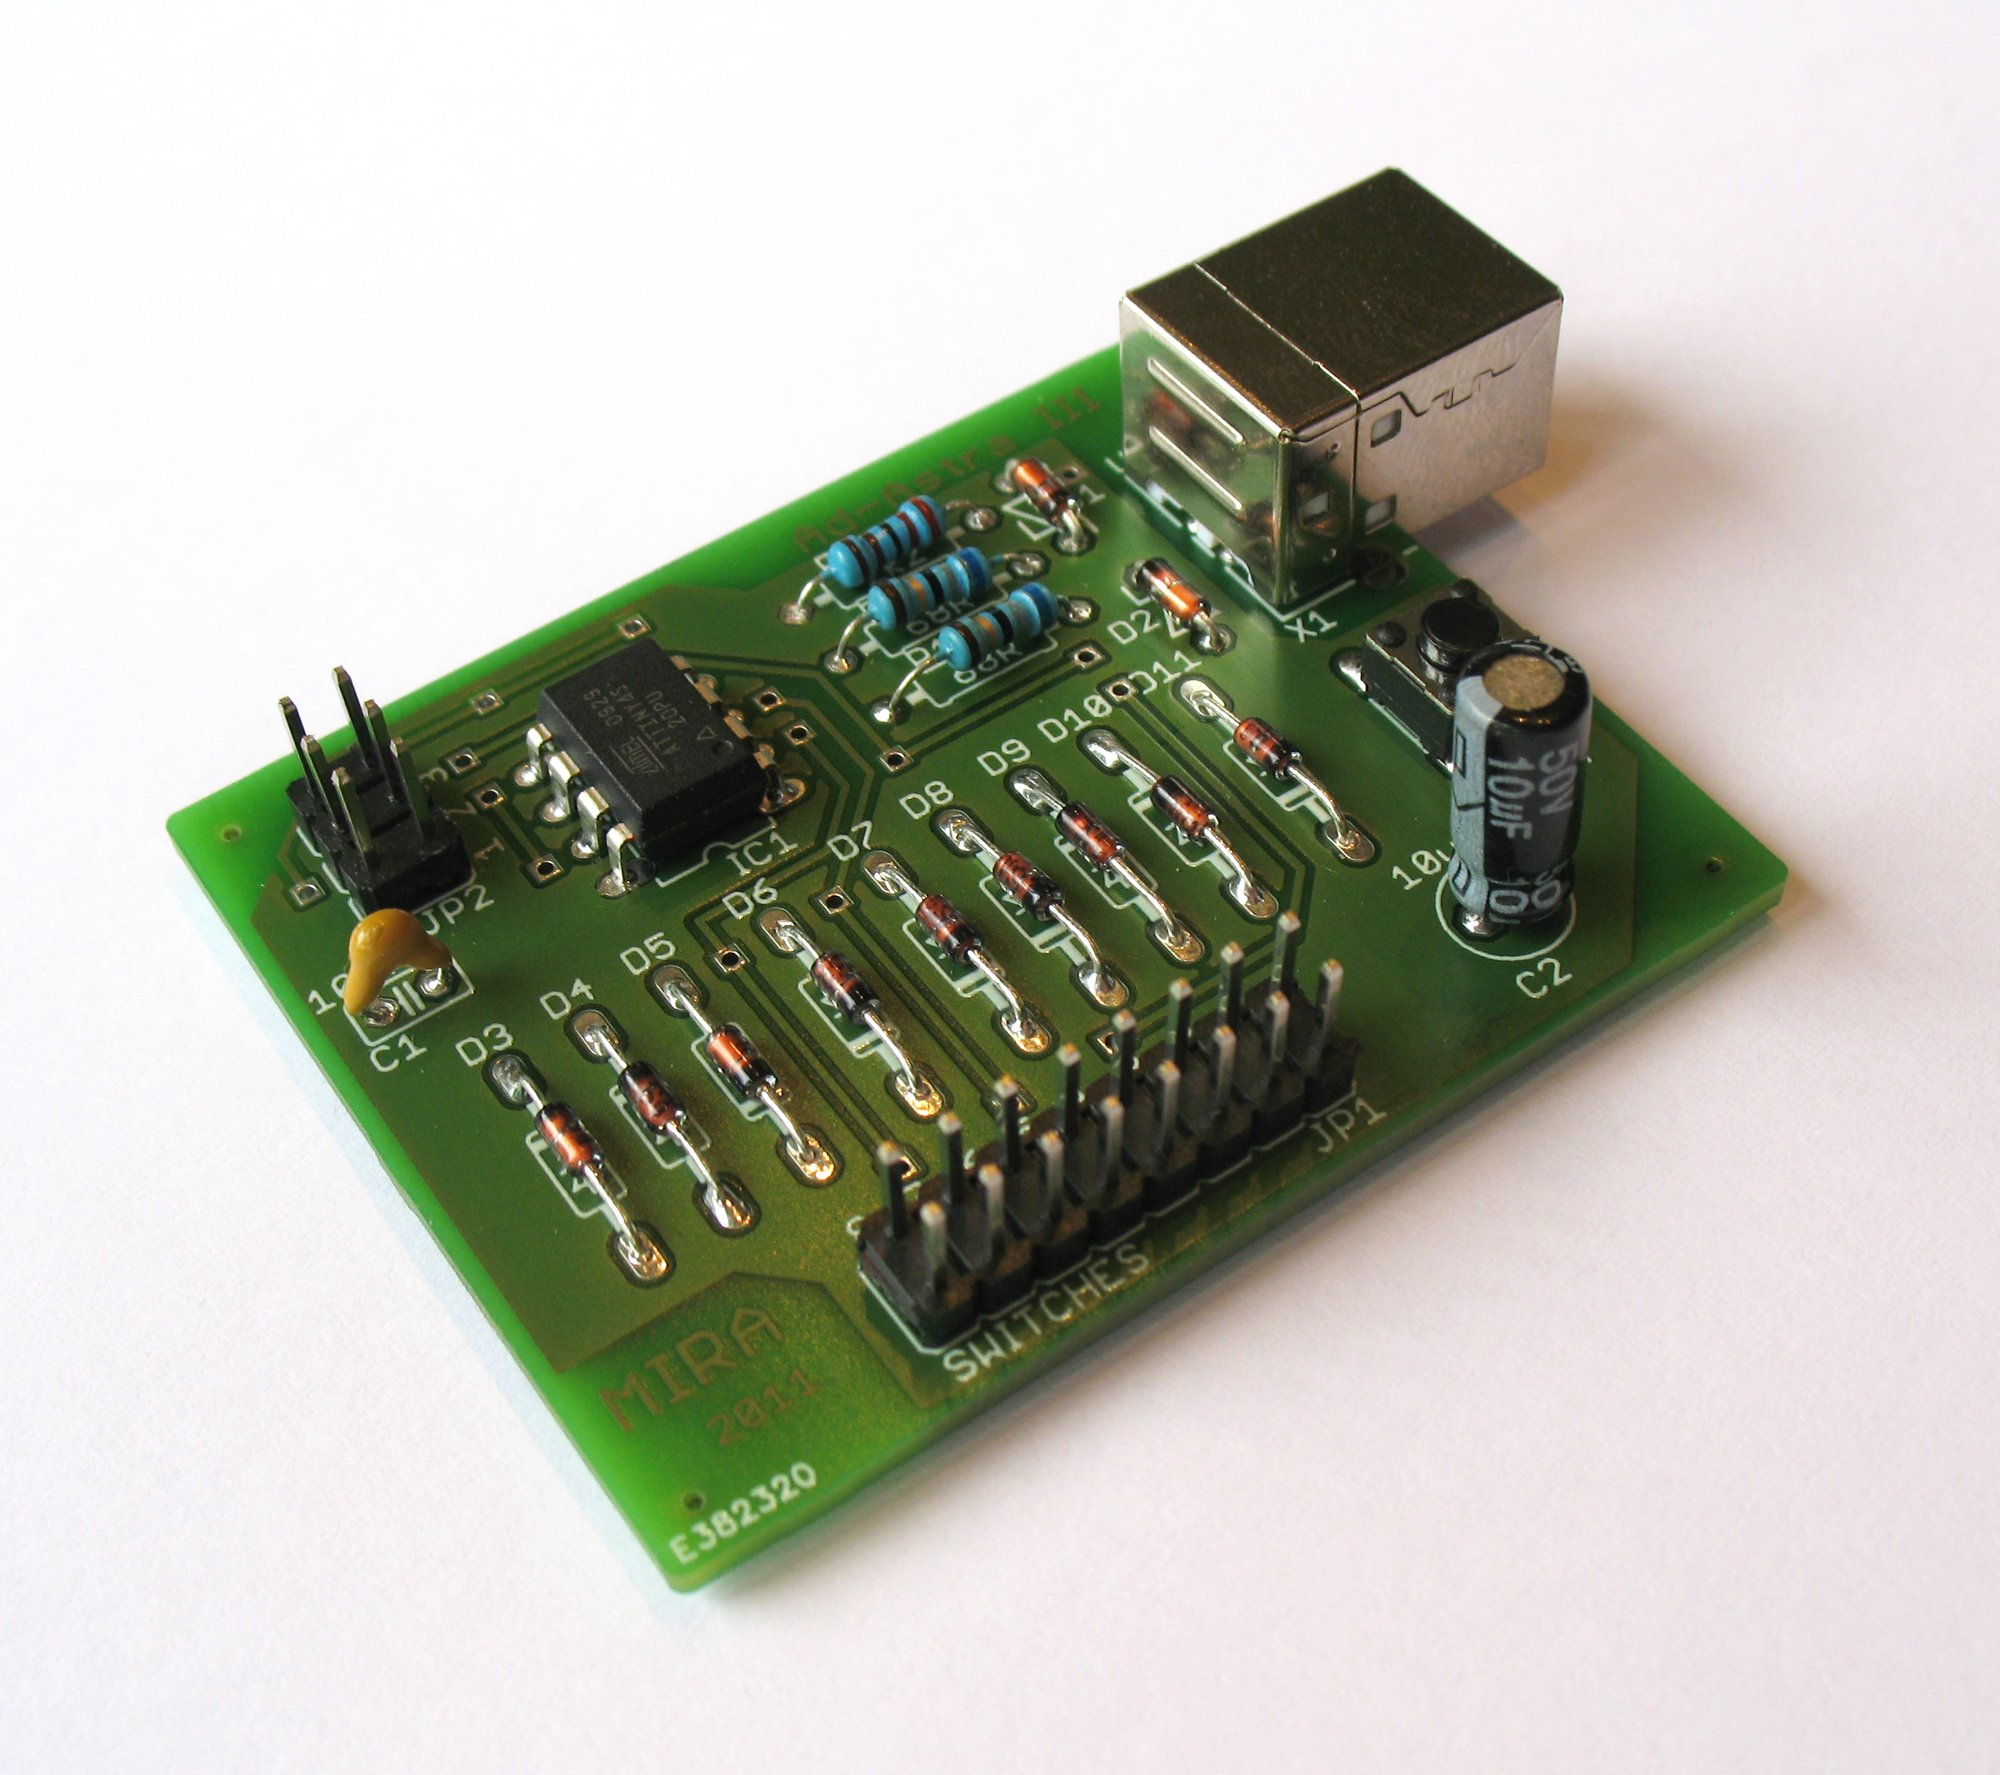
\includegraphics[width=\textwidth]{afbeeldingen/inputmodule_afgewerkt}
	\caption{Finale versie van de inputmodule}
	\label{fig:inputmodule}
\end{figure}


\chapter{Firmware}
\label{inputmodule:firmware}

\section{Geheugengebruik}
\label{inputmodule:firmware:geheugengebruik}

Bij het schrijven van de firmware moesten we rekening houden met de mogelijkheden van de chip. Deze eigenschappen, vermeld in sectie \ref{inputmodule:hardware:microcontroller}, waren vaak sterk beperkend. Zo hadden we maar 4 kilobytes tot onze beschikking, waardoor het moeilijk zou worden om (een subset van) C++ te gebruiken: de overhead teweeggebracht door het gebruik van klassen is immers te groot. Ook moesten we erop letten om geen \emph{floating-point} berekeningen uit te voeren: aangezien de AtTiny45 geen \ac{fpu} bevat, zou het gebruik ervan resulteren in het meelinken van een \ac{fpu}-emulator (die ruim 2 kilobytes groot is).

Ook moeten we rekening houden met de beperkte hoeveelheid \ac{ram} geheugen. Een voorbeeld van een dergelijke optimalisatie is hoe we 14 bytes \ac{ram} geheugen uitgespaard hebben bij de lookup-table waarmee een bitmap van geactiveerde schakelaars geconverteerd wordt naar de geschikte toetsaandruk. Aangezien we over 7 schakelaars beschikken, en er 1 extra entry in de lookup tabel aanwezig is voor wanneer er geen toets ingedrukt is, hebben we 8 ingangen nodig binnen de lookup-table. Voor elke ingang in die tabel, die we indexeren met de bitmap om zo geen extra ruimte te vereisen, hebben we twee waarden nodig: de toets, en een modifier (zoals \code{shift} of \code{alt}). Beide waarden worden geëncodeerd als een \code{uchar}, en nemen dus elk 1 byte in beslag. Hierdoor is de hele lookup-table exact 16 bytes groot. Omdat we deze tabel rechtstreeks indexeren moet ze volledig in het \ac{ram} geheugen staan, zélfs als we ze nooit zullen wijzigen. Om deze verkwisting te vermijden zullen we gebruik maken van de \code{PROGMEM} macro die ons toelaat om bepaalde datastructuren onder dwang in het programmageheugen op te slaan. Hoewel we daardoor 16 bytes uitsparen, moeten we nu meer opletten bij het gebruik van de lookup-tabel: de tabel is niet langer rechtstreeks te indexeren. Meer concreet: pointers die we berekenen door het optellen van een offset (de bitmap waarmee we normaal de tabel indexeerden) met het basisadres van de tabel mogen we nu niet langer rechtstreeks gebruiken om gegevens om te halen (\emph{pointer dereferencing}), maar enkel voor aanroepen van de \code{pgm\_read\_word} functie. Het resultaat, nu slechts 2 bytes groot, dienen we natuurlijk op te slaan in \ac{ram} geheugen.

\begin{lstlisting}[language=C, float, caption=Optimalisatie van de lookup-table.]
static const uchar keyReport[NUM_KEYS+1][2] PROGMEM = {
/* none */  {0, 0},
/*  1 */    {MOD_SHIFT_RIGHT, KEY_1},
/*  2 */    {MOD_SHIFT_RIGHT, KEY_2},
/*  3 */    {MOD_SHIFT_RIGHT, KEY_3},
/*  4 */    {MOD_SHIFT_RIGHT, KEY_4},
/*  5 */    {MOD_SHIFT_RIGHT, KEY_5},
/*  6 */    {MOD_SHIFT_RIGHT, KEY_6},
/*  7 */    {MOD_SHIFT_RIGHT, KEY_7},
};

static void handleKeyPress(uchar key)
{
    *(int *)data = pgm_read_word(keyReport[key]);
}
\end{lstlisting}

Tenslotte gebruiken we ook nog 1 byte uit het \ac{eeprom} geheugen om het resultaat van een succesvolle kalibratie in op te slaan. Die kalibratie is, zoals beschreven in sectie \ref{inputmodule:hardware:microcontroller}, nodig omdat we geen oscillator gebruikt hebben op de printplaat. Omdat die kalibratie echter enige tijd in beslag neemt, slaan we het resultaat ervan op zodat na een heropstart de kalibratie niet opnieuw moet uitgevoerd worden.

Na verschillende optimalisaties ziet het geheugengebruik er als volgt uit:
\begin{table}[h!]
  \begin{center}
    \begin{tabular}{c c c}
    Geheugen & Gebruik & Limiet \\
    \hline
    Flash & 2172 bytes & 4 kilobytes \\
    \ac{ram} & 61 bytes & 256 bytes \\
    \ac{eeprom} & 1 byte & 256 bytes \\
    \end{tabular}
  \end{center}
  \caption{Geheugengebruik van de firmware voor de inputmodule}
\end{table}

\section{Codeanalyse}
\label{inputmodule:firmware:codenalyse}

Net zoals we bij de kioskapplicatie een probleem hadden om de constructies specifiek aan Qt te analyseren, was het ook niet eenvoudig de code van de firmware te controleren. Het probleem hierbij is dat de code opnieuw gebruik maakt van een groot aantal macro's en symbolen gedefiniëerd door een complexe combinatie van AVR-specifieke headers en symbolen die via de command-line aan de preprocessor doorgegeven worden. Om dit te illustreren leggen we uit hoe je een bit uitschrijft naar de eerste pin van de eerste uitwendige poort. De code daarvoor is eenvoudig, en werkt op alle AVR microcontrollers: \code{PORTA = (1<<PA1);}. Hierbij zijn er twee speciale symbolen in het spel: \code{PORTA} die naar de juiste I/O-registers van de poort wijst, en \code{PA1} die indiceert hoeveel plaatsen de bit moet opgeschoven worden om terecht te komen op het gedeelte van het I/O-register dat wijst naar de eerste pin van de poort.

Het is duidelijk dat exacte inhoudt van deze registers verschilt van model tot model, en die symbolen gebruikt worden om de code enigszins overdraagbaar te houden. Wanneer de code echter gecompileerd wordt, moeten deze symbolen vervangen worden door de juiste geheugenadressen en waarden. Daarvoor zorgen de headers uit de AVR C-library, tegelijk een mooie illustratie van de mogelijkheden die de C preprocessor biedt. Een illustratief voorbeeld van hoe de het \code{PA1} symbool door de preprocessor zal omgezet worden, is zien in fragment \ref{lst:avr:preprocessor}.

\begin{lstlisting}[language=C, float, caption=Omzetten van AVR symbolen via preprocessor-logica., label=lst:avr:preprocessor]
#ifndef _AVR_ATTINY13A_
  #define PA1 2
  #define PA2 1
  #define PA3 0
#elif _AVR_ATTINY45PU_
  #define PA1 0
  #define PA2 1
  #define PA3 2
  #define PA4 4
#else
  #error Unknown microprocessor model.
#endif
\end{lstlisting}

Zoals te zien is in fragment \ref{lst:avr:preprocessor} berust de preprocessor op enkele symbolen die door de programmeur moeten gespecificeerd worden. Die symbolen moeten gedefiniëerd zijn wanneer de preprocessor de code verwerkt, wat in de praktijk vaak gedaan wordt door een header te includen (bijvoorbeeld \code{settings.h}) die als enige taak heeft die kritieke symbolen te definiëren. Wij hebben er echter voor gekozen om de symbolen door te geven aan de compiler en preprocessor via de command-line, waardoor we alle configuratie kunnen isoleren binnen de \code{Makefile}.

Het grote probleem met al deze preprocessor-logica is dat statische analyse-tools er vaak niet goed mee overweg kunnen. Het is ook geen oplossing om eerst de preprocessor zijn werk te laten doen omdat de code dan vaak niet meer herkenbaar is en het voor de programmeur dan niet te doen is om de output van de analysetools correct te interpreteren. Daarom hebben we, zeker gezien de beperkte grootte van de firmware (nog geen 250 regels code) besloten om niet verder te zoeken naar analysetools en gewoon zelf de code eens extra grondig te controleren.

\section{Compilatie}
\label{inputmodule:firmware:compilatie}

Het grote probleem bij het compileren van de firmware is dat de machinecode die de AVR microcontroller vereist niet compatibel is met de x86-machinecode die een compiler op onze computers gegenereerd. We zullen dus een compiler moeten gebruiken die specifiek geconfigureerd is om machinecode te genereren die kan draaien op een ander systeem dan hetgeen waar de compiler op uitgevoerd wordt. Dit proces heet \emph{cross compiling}.

Als we kijken naar de bekendere open-source compilers is de AVR versie van \ac{gcc} de de-facto standaard voor het compileren van code voor AVR microprocessoren. Ook zou het gebruiken van een andere compiler ervoor zorgen dat we flink wat code zouden moeten converteren om überhaupt nog te compileren. Veel van de preprocessor-logica beschreven in sectie \ref{inputmodule:firmware:codenalyse} is immers geïmplementeerd met \ac{gcc}-specifieke instructies (ook wel \emph{compiler intrinsics} genoemd). Als we bijvoorbeeld naar een andere kwalitatieve compiler kijken, IAR's Embedded Workbench, moeten we zelf afhankelijk van het model microprocessor bepalen welke header we gebruiken, en is het natuurlijk niet mogelijk om daarvoor de \ac{gcc} headers te gebruiken die wel voorzien in een handige abstractielaag.

Om toch toch nog enigszins aan codeanalyse te doen hebben we vervolgens \ac{gcc} dusdanig geconfigureerd dat het zoveel mogelijk potentiële fouten detecteert en uitschrijft. Dit hebben we gedaan met de \code{-Wall} en \code{-Wextra} parameters, waarmee we een probleem hebben ontdekt betreffende pointer uitlijning.
 
\part{Voorstellingen}
\label{voorstellingen}

\chapter{Prototype}
\label{voorstellingen:prototype}

Hoewel het uiteindelijk de taak van een designer is om voorstellingen te ontwikkelen die ten volste gebruik maken van het framework, zullen we toch een aantal voorstellingen ontwerpen die gebruikt zullen worden in de eerste toepassing van het systeem. De eerste daarvan zal gebruikt worden binnen de prototype kiosk, en zal dienen als demonstratie van de mogelijkheden die het nieuwe framework biedt. Dat kunnen we best doen met een specifiek daarvoor ontworpen demo, zoals er wel veel zijn sinds de opkomst van het \emph{Web 2.0} (een term die duidt op webpagina's gemaakt in \ac{html} versie 5, \ac{css} en Javascript).

Omdat het past binnen de situering van ons project, zullen we gebruik maken van de \makeurl{https://mozillademos.org/demos/planetarium/demo.html}{Planetarium} demo, gevonden in de Web ‘O Wonder suite. Die demos zijn begin 2011 ontworpen door Mozilla om de mogelijkheden en kwaliteit van de vierde iteratie van hun Firefox browser aan te tonen. Daarbij heeft Mozilla voornamelijk gebruik gemaakt van volledig gestandaardiseerde technologieën \citep{webowonder}, waardoor de Planetarium demo vrijwel vlekkeloos werkt in andere browsers, of meer specifiek andere rendering engines (zoals de Webkit engine die wij gebruiken).

Hoewel we op vlak van technologie geen aanpassingen hebben moeten doorvoeren, was dit wel nodig om compatibel te zijn met de methode van gebruikersinput die wij hanteren. Zo zullen de kiosken niet uitgerust zijn met een muis, maar enkel met 4 pijltjestoetsen. Gelukkig kon het gros van de demo reeds overweg met pijltjestoetsen, we hebben enkel moeten toevoegen dat de twee verticale pijltjestoetsen ervoor zorgden dat de taal van de pagina veranderde, en dat na het laden van de pagina direct overgegaan werd tot het perspectief waarin de demo overweg kan met de horizontale pijltjestoetsen (standaard startte de pagina immers in een overzichtsperspectief).

\chapter{Meta voorstelling}
\label{voorstellingen:metavoorstelling}

De tweede voorstelling die we voorzien hebben is eerder een hulpmiddel dan effectieve voorstelling, en dient er enkel toe om de bestaande voorstellingen te kunnen gebruiken binnen het nieuwe framework. Zoals beschreven in sectie \ref{ontwerp:applicatie:voorstellingen} zullen we daartoe eerst de bestaande videofragmenten comprimeren met een videocodec waardoor transmissie over het netwerk toch al iets efficiënter verloopt. De keuze van videocodec is dan uiteindelijk gevallen op WebM, om zo toe te laten om eenvoudig de videofragmenten zonder extra plugins te kunnen afspelen uit \ac{html} 5 code via het \code{<video>} element.

Maar er is meer nodig dan een methode om de fragmenten af te spelen. Zo moet het mogelijk zijn om verschillende fragmenten aan te bieden, en de bezoeker er uit te laten kiezen. Ook moet het mogelijk zijn een fragment te voorzien van ondertitels, waarbij dan natuurlijk ook moet geselecteerd worden in welke taal die moeten zijn.

\section{Template pagina}
\label{voorstellingen:metavoorstelling:template}

Om dit te realiseren hebben we eerst een \emph{single-page} \ac{html} pagina ontworpen waarbij alle basiselementen aanwezig zijn: een header die het logo van de MIRA en de titel van de voorstelling bevat, een footer waarin een hint kan staan voor de bezoeker (zoals op welke knop hij moet duwen om een keuze te bevestigen), en tenslotte het centrale gedeelte van de pagina waarin de effectieve inhoud zal komen.

Die inhoud wordt per sectie onderverdeeld via het \ac{html} \code{<div>} element. Elk van die onderverdelingen heeft een uniek id, waardoor er vanuit de code kan naar verwezen worden. Die code zal ervoor moeten zorgen dat eerst de taalselectie-pagina zichtbaar is, er na keuze van een taal doorgegaan wordt naar de pagina waar de bezoeker een fragment kan kiezen, om vervolgens dan ook het fragment daadwerkelijk te tonen.

\section{Applicatielogica}
\label{voorstellingen:metavoorstelling:logica}

Om die logica te implementeren zullen we Javascript code moeten schrijven die uitgevoerd wordt wanneer de pagina geladen wordt, en wanneer de bezoeker bepaalde acties onderneemt. Om het schrijven van Javascript code specifiek gericht op \ac{html} pagina's te vereenvoudigen, maken we gebruik van de \makeurl{http://jquery.com/}{jQuery} bibliotheek. Hiermee wordt het onder andere veel eenvoudiger om specifieke \ac{html} elementen op te halen en op events te reageren, zoals geïllustreerd is in fragment \ref{lst:jquery:selector}.
\begin{lstlisting}[language=Javascript, float, caption=Ophalen van een element met en zonder hulp van JQuery., label=lst:jquery:selector]
function countCheckedElements_jQuery()
{
	return $("#myForm input:checked").length
}

function countCheckedElements()
{
	var form = document.getElementById('myForm')
	
	var count = 0
	for (i=0; i < form.elements.length; i++) {
		var type = form.elements[i].type
		if (   type == "input"
		    && form.elements[i].checked ) {
			count++;
		}
	}
	
	return count
}
\end{lstlisting}

Met behulp van jQuery hebben we vervolgens een aantal functies geschreven die toelaten om de template pagina die we daarnet gedefinieerd hebben, in te vullen. Zo hebben we bijvoorbeeld voorzien in een \code{setTitle} methode die toelaat de titel van de pagina in te vullen, of \code{setStatus} om het statusbericht dat in de footer terecht komt te veranderen. Hiermee wordt het een pak aangenamer om de uiteindelijke applicatielogica te implementeren.

\section{Taalkeuze en internationalisering}
\label{voorstellingen:metavoorstelling:taal}

Het eerste dat we de bezoeker moeten vragen, is in welke taal de volgende pagina's en het uiteindelijke fragment moeten gepresenteerd worden. Hoewel dit niet meer is dan een aantal eenvoudige checkboxes, heeft de keuze verregaande implicaties. We zouden er zo voor kunnen kiezen om afhankelijk van de taalkeuze door te gaan naar verschillende pagina's, maar dat impliceert veel dubbel werk aangezien we nu pagina's met dezelfde inhoud en logica zullen moeten dupliceren per mogelijke taalkeuze.

Daarom hebben we er voor gekozen om gebruik te maken van \makeurl{http://keith-wood.name/localisation.html}{een jQuery plugin} die de bibliotheek uitbreidt met een aantal vertalingsfuncties. Die functies zijn eigenlijk heel eenvoudig, en laten toe om aan de hand van een uniek id een gelocaliseerde string op te halen. Dit zou wel betekenen dat we bij het laden van een pagina manueel de inhoud van elk vertaalbaar element moeten vervangen door het resultaat van een aanroep naar die plugin, wat veel extra regels code zou betekenen. Daarom hebben we voor een andere aanpak gekozen, waarbij we elk element voorzien van een uniek id en bij het inladen van de pagina een jQuery selector nu de hele pagina automatisch overloopt om voor elk element te kijken of zijn id overeenkomt met een geregistreerd id binnen de vertalingsplugin. Is dit het geval, dan zal de waarde van dat element (waarvan de betekenis verschilt van element tot element) gelijk gesteld worden aan de vertaling die de plugin teruggegeven heeft.

\section{Playback en ondertiteling}
\label{voorstellingen:metavoorstelling:playback}

Nu deze taal vastligt moet de bezoeker kunnen kiezen uit de verschillende fragmenten, die vervolgens moeten afgespeeld worden met ondertitels in de taal die hij gekozen heeft. Afspelen van een video is relatief eenvoudig, we moeten enkel het ``src'' attribuut van het video-element wijzigen zodat het gekozen fragment ingeladen wordt, en er tenslotte de \code{play()} functie op aanroepen.

Ondertitels inladen is minder eenvoudig, omdat het \ac{html} video-element daar geen ondersteuning toe biedt. Opnieuw gaan we gebruik maken van \makeurl{http://plugins.jquery.com/node/11465}{een jQuery plugin} die ons hierbij zal helpen, door een speciaal tekstelement gesynchroniseerd met het video-element correct in te vullen met de juiste ondertitels. Die moeten voor deze plugin opgemaakt zijn in de de facto standaard voor ondertitels, zijnde het \ac{srt} formaat.


\appendix

\backmatter
\chapter{Conclusie}

% todo: mag niet teveel op abstract lijken
% http://www.dissertationswriting.co.uk/dissertation_conclusion.htm 

Het doel van deze thesis was de ontwikkeling van een modern multimediaframework dat zorgt voor de opslag, distributie en weergave van multimediafragmenten op de kiosken van de volkssterrenwacht MIRA. Daarbij is belangrijk dat een beheerder elk van die processen voldoende kan opvolgen en beïnvloeden, zonder al teveel technische kennis nodig te hebben. Ook moet het mogelijk zijn om mooie voorstellingen te realiseren met de middelen die het platform aanbiedt, en tegelijk compatibel te zijn met de voorstellingen die momenteel gebruikt worden.

We hebben ervoor gekozen om de voorstellingen op te maken in \ac{html} en Javascript, waarmeer we zeer rijke gebruikerservaringen kunnen ontwerpen. Ook compatibiliteit met de huidige voorstellingen is ermee mogelijk: na conversie naar het WebM formaat kunnen we de fragmenten gebruiken binnen \ac{html}. Om daarbij dynamisch de taalkeuze van de gebruiker in te verwerken hebben we voorzien in een kleine webapplicatie, opgebouwd met behulp van JQuery.
Vervolgens worden de voorstellingen opgeslaan in een \ac{svn} repository, waardoor efficiënte overdracht bekomen wordt en een beheerder relatief eenvoudig wijzigingen kan doorvoeren aan de inhoud van de voorstellingen.

% server

% client

% inputmodule

% conclusie

% Bibliografie
\bibliographystyle{plainnat}
\bibliography{verslag}


\end{document}
